\documentclass[a4paper,12pt]{booksfsf}
%\documentclass[a4paper,12pt,twoside,fleqn]{booksfsf}

\usepackage{hyperref}
\usepackage{latexsym}

\usepackage{graphics}
\usepackage{graphicx}
\usepackage{amsmath}
\usepackage{psfrag}   
\usepackage{cite}
\def\citepunct{], [}
\def\citedash{]--[}

\usepackage{pdfpages}                           % To allow inclusion of the frontpage as a pdf-page
\usepackage{caption}   
\usepackage{captspec}
\usepackage[printonlyused]{acronym} 
\usepackage{makeidx} 
\usepackage[english]{babel} 
\makeindex  
\usepackage{color}
\usepackage{tabularx}
\usepackage{amsbsy}
\usepackage{lscape}
\usepackage{breakurl}
\usepackage{appendix}

\usepackage[labelfont = it, font = footnotesize, hangindent = 26pt, parskip = 20pt]{subfig}
\usepackage{enumerate}

\setlength{\oddsidemargin}{0.746cm}
\setlength{\evensidemargin}{-0.1in}
\setlength{\textwidth}{15.5cm}
\setlength{\topmargin}{-0.45in}
\setlength{\headheight}{0.3in}
\setlength{\headsep}{0.35in}
\setlength{\textheight}{24cm}
\setlength{\footskip}{0.4in}

\renewcommand{\baselinestretch}{1.20}
\renewcommand{\captionfont}{\footnotesize\itshape}

\renewcommand\sfdefault{phv}                               % use helvetica for sans serif
\renewcommand\familydefault{\sfdefault}               %    use sans serif by default


\begin{document}

\frontmatter 


\includepdf{frontpage} % Include the frontpage which is a separate pdf. Make sure the pdf exists!
                       % Note: this only works with PDFlatex. If you use a different typesetter,
                       % then include the frontpage afterwards, e.g. using Adobe Acrobat

\pagestyle{empty}

%\

%\newpage
%\cleardoublepage

\chapter{Preface [optional]}
\pagestyle{headings}

The preface is optional. It contains anything that is outside the actual scope of the report, for instance
\begin{itemize}
	\item how you ended up doing the assignment that is reported in this document;
	\item your personal opinion on the subject;
	\item an acknowledgment to the people that helped you carrying out the work.
\end{itemize}
Alternatively an epilogue or acknowledgment chapter could be included in the backmatter of the report.

\chapter{Summary}
\pagestyle{headings}

This research set out to investigate the feasibility of performing Emotion-Recognition using Melomind, a wearable neural interface manufactured by myBrainTechnologies. Melomind is capable of recording EEG signals, that can be processed using machine learning algorithms in the form of a classification task of the emotional dimensions of valence and arousal.

This study introduces the fields of Brain-Computer Interfaces and Affective Computing, the perception of the market, the leading companies producing wearable neural devices for non-clinical applications and the relevance of studying emotions using music, from both the perspectives of market demand and enhancing the user experience.

The goal of this research was to evaluate Melomind's capabilities for a future real-time application that can be used to perform Emotion-Recognition. In order to do so, the Valence-Arousal model by James Russel was used as metric for the dimensions of emotions, then several models of emotional correlates in brain activity were evaluated to define what features of the EEG would be more suitable for the task.

The relevant related work was reviewed and studied to provide a methodological framework for the machine learning task that could be adapted to the constraints imposed by the limited hardware of the Melomind. An experimental protocol was designed around the inherent advantages of wearable technologies to collect a dataset with continuous labelling of emotions on the Valence-Arousal coordinate system. Possible biases caused by listening conditions, data labelling tools, emotional interference, multiple cognitive tasks and external factors were taken into account and the protocol was tested during a pilot week with employees of myBrainTechnologies prior to the real experiment.

Data were collected using a robust protocol in two different conditions for music listening: eyes-open with a labelling task and eyes-closed solely. Data were then processed using a lightweight automated preprocessing pipeline and two types of features were extracted from the Power Spectra Density of the EEG signal: neuromarkers and frequency-band specific spectral properties calculated in the Theta, Alpha and Beta bands of the EEG signal. Features dimensionality was reduced through features extraction using Principal Component Analysis and the classification task was performed with subject-dependent strategy. The problem was simplified into two separate binary classifications tasks for valence and arousal, and two supervised learning algorithms were tested: Support-Vector Machines and Multi-Layer Perceptron. The hyper-parameters were tuned using GridSearch to select the configuration that yielded the highest Matthews Correlation Coefficient score for each participant, a coefficient that is gaining popularity in machine learning research thanks to its higher reliability. 

All models were then trained and tested using 5-fold leave-one-block-out cross-validation that produced two cross-validated scores on the training datasets: CV accuracy and CV MCC. Then, models were further tested on a completely unseen split of data that produced two more scores: test accuracy and MCC. Results were collected and the two classification methods were compared with each other and then with the comparable related work. 

Some models showed promising classification results, reaching ~80\% accuracy in arousal classification and ~75\% accuracy in valence classification with both SVM and MLP. MCC scores confirmed an average positive learning capability of the models, although many models ended up overfitting or underfitting. The average classification results did not meet the initial expectations and are below many of the related studies, suggesting that the adopted lightweight pre-processing, the limited hardware of the Melomind or a combination of both are hindering the classification task and are not yet suitable for real-time Emotion-Recognition.

The final discussion covers the current challenges of real-time Emotion-Recognition reported by this and related studies and delves into possible improvement of the emotional self-reporting, the features selection, the artifacts cleaning process and the requirements to move from subject-dependent classification to subject independent-classification.

In the conclusion, some considerations are raised from answering the research questions and then an improved artifact cleaning approach is recommended for a follow-up study using the same dataset, that could give further insights on the development of a wearable affective Brain-Computer Interface using Melomind.



\tableofcontents

\chapter{List of acronyms}

\begin{acronym}[TDMAAA]
	%\setlength{\itemsep}{5cm}
	\acro{IEEE}				{Institute of Electrical and Electronics Engineers}
	\acro{AC}				{Affective Computing}	
	\acro{AI}				{Artificial Intelligence}
    \acro{ER}			   {Emotion-Recognition}
    \acro{BCI}			   {Brain-Computer Interface}
    \acro{BCIs}			   {Brain-Computer Interfaces}
    \acro{EEG}			   {Electroencephalography}
    \acro{fMRI}           {Functional Magnetic Resonance Imaging}
    \acro{fNIRS}          {Functional Near-Infrared Spectroscopy}
    \acro{MEG}           {Magnetoencephalography}
    \acro{EP}           {evoked potentials}
    \acro{ERPs}		  {event-related potentials}
    \acro{PPG}        {photoplethysmogram}
    \acro{VA}        {valence-arousal}
    \acro{SAM}		{Self-Assessment Mannikin}
    \acro{PANAS}		{Positive And Negative Affect Scales}
    \acro{AWI}		{Approach-Withdrawal Index}
    \acro{FMTI}		{Frontal Midline Theta Index}
    \acro{SASI}		{Spectral Asymmetry Index}
    \acro{DFT}		{Discrete Fourier Transform}

\end{acronym}



\mainmatter

\chapter{Introduction}
\label{chap:introduction}

The evolution of technology is inherently bound to the evolution of society and human desires. In recent years the focus of the technology-mediated services has shifted from mere functionalism to become more aesthetically, functionally, socially, and interactively pleasurable. The most successful multimedia creation and distribution companies offer customized recommending services and then aggregate correct predictions between users sharing similar taste or preferences to improve their offer: an experience as tailored as possible to users' individual needs. Understanding users’ behavior and emotions is not only very profitable for companies that want to continuously engage their users, but also a popular topic among researchers and designers that thrive to better understand the human mind to enhance the quality of human-computer interactions. It is also becoming a necessity for the end users themselves, who are not satisfied anymore by tinkering with technology but want the interaction to be flexible and seamlessly usable in the daily life. Recent applications and services offer the possibility for people to monitor their body, mind, and health through continuous collection of physiological signals from wearable sensors, for example to keep track of good sport habits, sleep quality, stress level and more. But it is also possible to infer affective states from clues in the recorded brain activity. Given the increasing interest of researchers and companies in the affective field, the more and more frequent use of physiological and behavioral clues to assess mental states will keep growing until technologies of daily use will be standardly designed with brain-reading capabilities. The human brain is the central and most important organ of our body because it is where our consciousness, our “self”, resides and it is the command center of all vital functions. And yet, it is also the one we understand least, despite the ongoing research. We rightfully assume emotions originate in the brain, but we can only observe their physiological responses and we can only qualitatively support these observations through inherently imprecise self-assessment tools. Trying to find a correlation between the physiological response and the self-assessed mental state or emotion is not as simple as correlating factual measures, because of the uncertainty of the factors involved. Modern wearable \ac{BCIs}, mostly represented by EEG-capable devices, are still limited in their functionalities and design. Recorded signals are often affected by noise or artifactual information and the user experience is so heavily hindered that most companies are reluctant in investing into them, and more research and optimization is needed before pushing them to the general public. Self-assessing emotions is also non-trivial because it requires a strong understanding of one’s perceived emotions, and this perception has great variability from individual to individual. Creating models able to generalize through all the subjective differences is complicated, especially with performances that enable designers to create enjoyable user experiences for everyone. Thus, we enter in a challenging and almost paradoxical situation: on one hand the goal is to find a common approach to exploit generic behavioral and physiological patterns, on the other hand it is also necessary to account for individual differences to offer the customized experience that users desire. This research takes an extra step into the challenge by evaluating what could be the classification performances of an affective \ac{BCI} system for emotion-aware recommendations using a wearable device. It delves on relevant insights on the main problematics that researchers and designers will face in the years to come when classifying brain emotions, and finally discusses possible solutions and future developments towards online Emotion-Recognition.

\section{Motivation}
\label{sec:motivation}
In 2016, the American research and advisory information firm Gartner published their yearly hype cycle for emerging 
technologies , positioning “Brain-Computer Interfaces” and “Affective Computing” on the growing slope of the “Peak of Inflated Expectations”, both with an estimated period of about 10 or more years before mainstream adoption (see Figure \ref{fig_hype_cycle}).
\begin{figure}[ht]
%Insert your figure here. Make sure that the type of figure file (eps/pdf/...) complies with your typesetter.
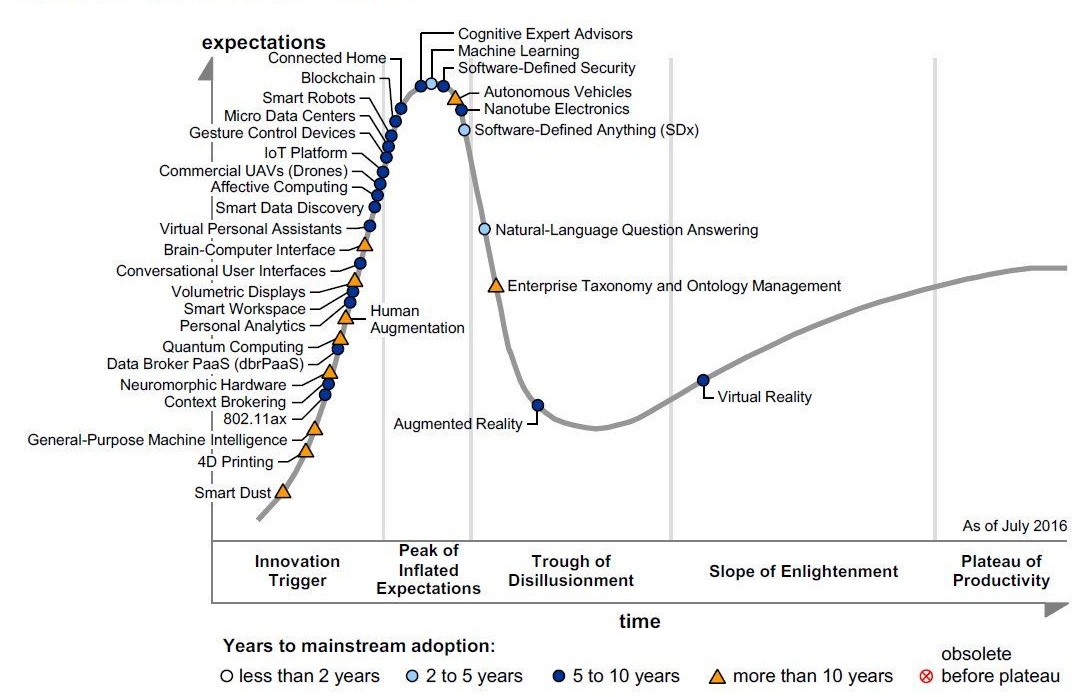
\includegraphics[width=\textwidth]{img/intro/hype_curve_trim.jpg}
\caption{Gartner hype cycle for emerging technologies in 2016, from Gartner\cite{noauthor_gartners_nodate}}\label{fig_hype_cycle}
\end{figure}
In the versions published over the last 5 years, "Affective Computing" completely disappeared from the hype cycle and "Brain-Computer Interfaces" slowly climbed the slope before disappearing as well. This trend suggests that both fields reached the peak of the inflated expectations and fell down the “Through of Disillusionment” slope as the technology failed to meet the expectations of users, researchers, and investors. Nevertheless, some innovative companies and startups stepped up to the challenge and started a new innovation cycle by developing wearable neural sensors and slowly pushing again \ac{BCI} towards mainstream adoption. For example, NextMind\footnote{https://www.next-mind.com/}  released in early 2021 a wearable sensor for active control of multimedia applications and games. Muse\footnote{https://choosemuse.com/} instead developed several wearable \ac{BCIs} for neurofeedback during guided meditations, recently updated to be used for sleep tracking. Enophone produces EEG-capable headphones and recently made a partnership with BrainFlow to integrate their SDK and build affective applications for music listening \cite{parfenov_brainflow_nodate}. Melomind\footnote{https://www.melomind.com/en/product/melomind-en/} , the device used in the current research, is another EEG capable device with headphones and an application for neurofeedback training. Ontbo\footnote{https://ontbo.com/en/} already promises an application with their headphones to generate music playlists that can alter the level of motivation, relaxation, stress, and concentration in the brain activity. Major brands like Valve, Tobii and OpenBCI are collaborating to bring together the world of virtual reality and \ac{BCI} \cite{parfenov_openbci_nodate}, and Facebook is developing their own neural interfaces after acquiring the neurotech startup CTRL-Labs \cite{statt_facebook_2019}. In the academic world, we can find very recent papers that focused on affective music recommendations, for example Chang et al. \cite{chang_personalized_2017} proposed a recommending system to suggest the appropriate stress-relief music to the users based on the inferred stress level in their EEG, while Abdul et al. \cite{abdul_emotion-aware_2018} designed an emotion-aware system to correlate implicit emotional user tags and musical features. This reignited interest in affective applications and the development of a new generation of \ac{BCIs} supports the relevance in researching and developing now the methods and tools that will be used to design the affective systems of tomorrow. Given this context, music is one of the best elicitors for the field of Emotion-Recognition for a multitude of reasons: 
\begin{itemize}
\item It is a proven powerful elicitor that arouses instinctive physiological reactions in the human body.
\item It has been used for centuries to convey emotional meaning, and now more than ever even across cultures, social classes, and age groups.
\item The physiological emotional response is agnostic of the stimulus, thus findings on music-elicited Emotion-Recognition are theoretically transferrable to other applications.
\item The market of music recommending systems is flourishing and very competitive, with many companies taking part in the technological development of such systems.
\end{itemize}
The music-emotion experience is very personal and influenced by internal factors, such as tempo and pitch of a song, as well as external factors such as memories, context, or correlated events associated to a past pleasurable or unpleasurable experience. 
The proposal of this study is a novel approach to the Emotion-Recognition task using Melomind, a wearable and consumer-oriented \ac{BCI}. The goal is to investigate the feasibility and the performances of the classification task in realistic listening conditions to evaluate the future development of wearable \ac{BCIs} equipped with online Emotion-Recognition for daily use. Instead of focusing on the correlation between the musical features and the \ac{ERPs} in the brain, the approach of this research is to use emotion-labelled songs as elicitors to study the spectral properties of frequency bands associated with emotions in the \ac{EEG} signal. These spectral properties can be translated into features and used for the computation of neural biomarkers, called “neuromarkers” in this research, to be fed into a classifier for the classification of the emotional valence and arousal based on known patterns in the brain activity. To support the collected physiological data, participants have been asked to continuously self-assess their emotions in a coordinate system representing the emotional dimensions of valence and arousal. The research questions of this study try to fulfil the design requirements of exploring the performances of the Emotion-Recognition task using a wearable \ac{EEG}  headset, considering the disadvantages and the advantages of this specific technology. The dry electrodes of the Melomind in pair with the headphones form factor allow for a very quick and relatively comfortable setup, enabling the researcher to focus on the task and overall shorten the experimental sessions. Consequently, it was possible for a single researcher to collect data from 45 subjects over 15 days. This technology has also limited recording capabilities; thus, the quality and quantity of data is lower than what could be obtained with standard \ac{EEG} lab equipment featuring 32 wet electrodes headcaps. Furthermore, the position of the Melomind electrodes only allows recording signals from the frontal and/or the parietal regions of the cerebral cortex, limiting considerably the area of study. The data has been collected through an experimental phase as result of a collaboration between the University of Twente and myBrainTechnologies, the company that manufactures Melomind. The research was approved by the Ethics Committee Computer \& Information Science and the Dean of the EEMCS  faculty following the regulations in force at the University of Twente, with reference number RP 2021-43.


\section{Research questions}
\label{sec:goal}
To evaluate this novel approach, this study aims to answer the following main research question:
\\
\\
\textbf{RQ}: \emph{ “What are the accuracy and MCC scores of subject-dependent classification of music-elicited emotional valence and arousal in the EEG signal using SVM and MLP algorithms with Melomind?”}
\\
\\
The mains research question was then extended by the following sub questions to support possible design choices for a real-time music recommending system based on brain activity.
\\
\\
\textbf{SRQ1}: \emph{“What are the most relevant selected Power Spectral Density features to perform the Emotion-Recognition using SVM and MLP algorithms with Melomind?”}
\\
\\
\textbf{SRQ2}: \emph{“What is the best classification strategy applicable to the current software and hardware capabilities of Melomind using SVM and MLP algorithms?”}



\section{Report organization}
\label{sec:organization}
To answer these research questions, the main models for self-assessment of emotions have been studied, together with the existing models relating the two main dimensions of emotional valence and arousal to brain activity (see Chapter \ref{chap:background}). The most compelling related work in classification of music-elicited emotions has been reviewed (see Chapter \ref{chap:related_work}) and used as methodical foundation. An experiment was designed to collect data in two listening conditions  and a processing pipeline was implemented to extract features and to train classification algorithms that could produce comparable results with the related work (see Chapter \ref{chap:methods}). The results were then collected (see Chapter \ref{chap:results}) and discussed with a view to possible future developments (see Chapter \ref{chap:discussion}).

\chapter{Background}
\label{chap:background}

\chapter{Related work}
\label{chap:related_work}

\chapter{Methods}
\label{chap:methods}
This chapter describes the methods used to carry on the research, from the data collection to the preprocessing and the results of the analysis. It includes a brief description of the population that took part into the experiment, the experimental task and conditions, the procedure adopted, and the equipment used. Then it delves into the analysis process starting with the preparation and preprocessing of the data and concluding with the intermediate outcomes of the classification. As previouslyu mentioned, the experiment is the result of a collaboration between the University of Twente, that provided the space, the recruitment system and part of the recording equipment, and myBrainTechnologies that provided their EEG-capable Melomind headsets and the rest of the equipment. The experimental design was reviewed and adjusted for ethical approval by the Ethics Committee of the university with reference number RP 2021-43 and compliant with the safety measures to prevent the spread of the Covid-19 virus.

\section{Experiment}
\label{sec:experiment}
The experimental phase of the research was crucial for the proper evaluation of Melomind. Previous studies conducted internally at myBrainTechnologies provided the theoretical backbone to work with neuromarkers and music, however the datasets of the employees were collected with a different experimental setup that did not account for the continuous measurement of emotional valence and arousal, and in any case there was always a chance data could be biased by the previous knowledge these "expert" subjects had on the topic and the technology. A feasible alternative could have been the simulation of a wearable device, similarly to the approach taken by Wu et al. \cite{wu_estimation_2017}, but that was kept as emergency solution in case it was not possible to run an experiment under the safety restrictions enforced by the Covid-19 pandemic. However, the open datasets available online for emotion analysis \cite{koelstra_deap_2012,soleymani_multimodal_2012,soleymani_deam_nodate} are recorded with a very different equipment than the Melomind, that would have not properly reflected the challenges of using a wearable neural interface. Finally, the opportunity to conduct the study with the students of the University of Twente and the availability of myBrainTechnologies to ship all the technical and hygienic materials to the Netherlands made it possible to proceed with the experimental protocol in the desired conditions.

\subsection{Experimental Annotation app for data collection}
\label{sec:experimental_annotation_app}
An app was developed to collect continuous annotations of perceived emotion, inspired by the design of the FEELTRACE tool \cite{cowie_feeltrace_2000} and the app developed by Thammasan et al. \cite{thammasan_continuous_2016}. The \ac{EA} app was developed in Python using the Psychopy\footnote{https://www.psychopy.org/}  engine for experimental behavioral sciences. The app is a collection of timed routines that alternate guided instructions, annotation tasks on a simplified GUI representing the valence-arousal space and Likert scales to report familiarity/liking scores in the range [1-5]. Three training sessions have been included:
\begin{itemize}
\item T1: the participant is presented with some background information about the \ac{VA} model and how to use the annotation tool.
\item T2: the participant is asked to annotate on the \ac{VA} space the perceived emotion while listening to 2 minutes of mixed music genres.
\item T3: the participant is presented with the simulation of a trial of the experiment, including reporting of familiarity/liking and the two listening conditions (see Chapter \ref{sec:task}).
\end{itemize}

The \ac{EA} app was designed and developed at myBrainTechnologies and then tested with the other employees during a short pilot period to adjust the instructions, the clarity of the GUI and the input method. Two input methods were evaluated with A/B testing methodology, using mouse and joystick respectively. The results of the test (see Appendix \ref{sec:appendix_A1}) confirmed that using mouse as input source required less training and effort, thus softening the cognitive load of the annotation task while music listening. Using the joystick would have enabled collecting annotation even in an eyes-closed listening condition thanks to the tactile feedback, but at the cost of requiring more training and concentration. To record experimental timed events, the \ac{EA} app was connected to the Melomind through a TriggerBox with an USB cable, a customized Arduino Nano board that can send binary-encoded labels using the serial port. 

\subsection{Participants}
\label{sec:participants}
In respect with the Covid-19 safety measures enforced by University of Twente, 45 healthy participants (28 females) participated in the experiment, all students, or ex-students of the university. The mean age of the population is 23.8 ± 3.1, with the oldest student being 31 years old and the youngest student being 18 years old at the time of the experiment (see Appendix \ref{sec:appendix_A2.1}). The lowest educational level was the enrollment as bachelor student and the highest educational level was having completed a master’s degree. Almost half of the participants (20) were Dutch, while all the rest came from different countries, but all of them had at least a C1 or equivalent English proficiency as requirement to enroll in University of Twente. Prior to be confirmed as participants, they were invited through an invitation form informing them on the nature of the experiment and collecting personal information such as demographic information, health conditions, drugs consumption, musical literacy, and some behavioral information on their habits in listening and searching for music to later support the design of a prototype. Almost 5\% of the participants reported to be left-handed, but none asked for an inverted setup of the equipment after it was offered to them (see Appendix \ref{sec:appendix_A2.1}). The only strict criterion to participate in the experiment was the capability to hear music, eventually through a hearing support system. None of the applicants was discarded nor required additional support for their health conditions. Prior to their experimental session, they were asked to refrain from consuming recreational drugs and alcohol in the 12 hours before the experiment and caffeine and tobacco in the hour before the experiment to prevent unexpected biases in the cerebral activity.

\subsection{Stimuli selection}
\label{sec:stimuli}
The stimuli were selected to represent an even as possible distribution of emotions according to the 4 classes identifiable by the quadrants of the Valence-Arousal space. These 4 classes are the possible combinations of positive and negative valence with high and low arousal. To keep consistency with related studies \cite{koelstra_deap_2012}, the classes have been named as follows going clockwise from the top-right quadrant:
\begin{itemize}
\item HAHV: High-Arousal and High-Valence.
\item LAHV: Low-Arousal and High-Valence.
\item LALV: Low-Arousal and Low-Valence.
\item HALV: High-Arousal and Low-Valence.
\end{itemize}
Selecting the right stimuli is a non-trivial task especially in the case of music since many factors can bias the personal perception. For example, familiarity with a certain song might elicit stronger emotions or create an effect of anticipation \cite{sangnark_revealing_2021}, \cite{ward_same_2013}, \cite{salimpoor_anatomically_2011}, while cultural biases or genre preference might completely change how a song is perceived \cite{chang_personalized_2017,fang_perception_2017}. Choosing to include lyrics or no lyrics may shift the attention of the listener from the meaning to the melody and vice versa. It is clearly hard to address all the possible issues but considering the scope of this study and the research on a realistic use-case scenario, most of these factors were either mitigated or considered with the due precautions. 

\begin{figure}[h!]
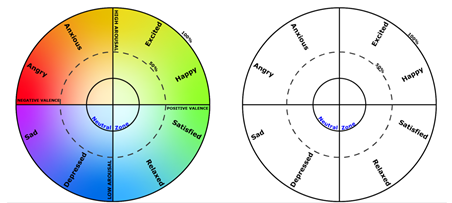
\includegraphics[width=12cm]{img/methods/va_space_experiment.png}
\centering
\caption{The Valence-Arousal space GUI used for the training with color cues on the left, and the uncolored Valence-Arousal space GUI used for the experiment session on the right.} \label{fig_va_space_experiment}
\end{figure}

The stimuli were finally selected as a subset of 8 songs (see Appendix \ref{sec:appendix_A2.2}) from the music database created by Koelstra et al. \cite{koelstra_deap_2012}, according to their emotional tagging. They used the popular online music database last.fm\footnote{https://www.last.fm/}  to retrieve 120 songs with associated music videos through their APIs, emotionally labelled by thousands of users. They then screened them down 40 stimuli during a web assessment session with at least 14 volunteers for each stimulus. The 8 songs selected for this study are a randomly picked subset of those 40 stimuli whose emotional web assessment belonged to the same Valence-Arousal quadrant as the last.fm tagging. For each quadrant there are exactly 2 songs and in total 8 emotions are supposedly portrayed: excitement, happiness, satisfaction, relaxation, depression, sadness, anger, and anxiety. 
It is important to point out that the web assessment conducted by Koelstra et al. was done using the music videos of these songs, and that the placement of the emotions in the \ac{VA} space used in this experiment (see Figure \ref{fig_va_space_experiment}) is a functional simplification of Russel's model \cite{russell_circumplex_1980}.

\subsection{Conditions}
\label{sec:conditions}
There is no common agreement in the academic world on which should be the best recording condition for an \ac{EEG} experiment about emotions, but most researchers agree on the minimization of external stimuli. Only few studies tried to assess the impact of recording in \ac{EO} condition and \ac{EC} condition on emotion analysis. Barry et al. reported \cite{barry_eeg_2007} differences in topography and power levels, due to the processing of visual input, and recommend considering them when choosing baseline conditions. Chang et al. \cite{chang_experiencing_2015} analyzed recording conditions in relation to music listening and reported that frontal Theta power significantly increased in the EC condition, while asymmetries indices in the Alpha power on parietal and temporal sites reflected emotional valence for \ac{EC} and \ac{EO} states respectively. In addition, participants rated music as more pleasant and more positive while listening with their eyes closed. These differences in the listening conditions did not seem to significantly impact on the current study that only used frontal electrodes but were considered in the design of the experimental task and in the choice of the resting state baseline. Another problem is caused by ocular movements and blinks that generates large artifacts in the EEG signal \cite{hagemann_effects_2001}. As a consequence, the data collected is of lower quality and requires more computationally expensive preprocessing. In the worst cases, some data must be pruned or reconstructed, varying from a few channels to the entire dataset of a participant. Eye artifacts are typically found in the data recorded by the electrodes placed on the frontal area of the scalp and are usually filtered away by subtracting \ac{EOG}, if recorded, from the \ac{EEG} signal. However it is not the case of this study that could not take advantage of extra sensors to record \ac{EOG} . In general, we can assume that an \ac{EC} condition yields better quality data than an \ac{EO} condition because the quantity of ocular artifacts will be reduced to the minimum and there is no underlying visual stimuli processing. The downsides of experimenting in the \ac{EC} condition are the obvious limitations on the task that could be presented to the participants and a possible increase of power in the Alpha band of the spectrum, that is usually amplified during resting and focused states. The main advantage of the \ac{EO} condition is the possibility to ask the participants for more complex tasks, at the cost of generating more ocular and muscular artifacts and eventually introducing multiple cognitive tasks at once, that can affect the analysis. Prior to the experiment, we run an internal pilot test at myBrainTechnologies to explore the best compromise options between having good quality data, the maximum amount of data and collecting the behavioral data we needed.
Thammasan et al. \cite{thammasan_continuous_2016} opted for a double listening protocol, in \ac{EC} condition to record \ac{EEG} and in \ac{EO} condition to collect affective annotations. This translates into listening twice to the same song but recording only in the \ac{EC} closed condition and then overlapping the annotations taken during the \ac{EO} conditions. Our limitation of 2 frontal electrodes already constrained the collectable amount of data, so we decided to extend this protocol with a double listening and recording approach, in both conditions. During the pilot we explored the feasibility of collecting annotations in both conditions using a joystick, but then opted for collecting annotations only during \ac{EO} condition with a mouse and then reuse the same annotations on the \ac{EEG} data collected in \ac{EC} condition.  As final consideration, the two conditions can be both present in realistic scenarios, with \ac{EO} being the most common listening condition, for example in an office or free-time scenario in which a user listen to music while performing other cognitive tasks (work, homework, gaming…). Listening in \ac{EC} condition resembles a more relaxed scenario, for example when listening to music at the opera or on a comfortable couch in the evening.

\subsection{Task}
\label{sec:task}
During the experimental session, participants were presented a main task during which their physiological signal were recorded. The task is divided into 3 sub-tasks for both conditions during each trial, with a total of 8 trials. The average length of the recording was approximately 35 minutes of recording. The sub-tasks in each trial, repeated for both conditions, were the following:

\begin{itemize}
\item Listening to white noise: before presenting the stimulus, participants listened to 15 seconds of white noise to “reset” their emotional state.
\item Listening to the stimulus in EO/EC conditions: participants listened to 60 seconds excerpts of each song. During the \ac{EO} condition participants were requested to continuously annotate their emotions on the \ac{VA} space, during the \ac{EC} condition they focused solely on the music. The order of presentation of the conditions depended on the assigned group.
\item Rating the stimulus: after listening to the song, participants were requested to give a rating in terms of familiarity and liking of the excerpts, using Likert scales ranging from 1 to 5. If for any reason they failed to give a score before the 20 seconds timer expired, the score would be automatically set to 3, that represented a neutral answer.
\end{itemize}
So, during each trial, the participants would listen to two different songs, rate them and only annotate during the \ac{EO} condition (see Fig. \ref{fig_experimental_trial}). 

\begin{figure}[h!]
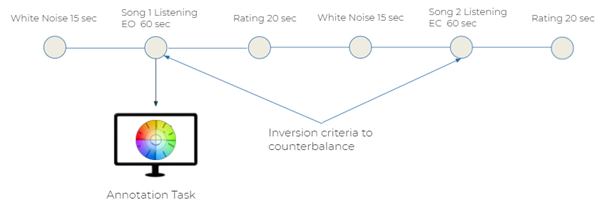
\includegraphics[width=12cm]{img/methods/experimental_trial.png}
\centering
\caption{Diagram of an experimental trial starting with EO listening condition.} \label{fig_experimental_trial}
\end{figure}

It is important to underline that the order of the conditions might induce some bias in the annotation task and the rating of each stimulus. To minimize the statistical effects, participants were randomly assigned to two groups in equal distribution, ECEO and EOEC, according to an inversion criterion that would determine the order in which the conditions were presented during the entire session. This solution seemed more elegant and less confusing than fully randomizing the order of the conditions for each trial, possibly creating confusion in the instructions. In addition, instead to presenting the same song consecutively in both conditions, we decided to split the session into two parts in which the stimuli are presented in pseudo-random class order in the first part, and then inverted in the second part as shown in Figure \ref{fig_inversion_criterion}.

\begin{figure}[h!]
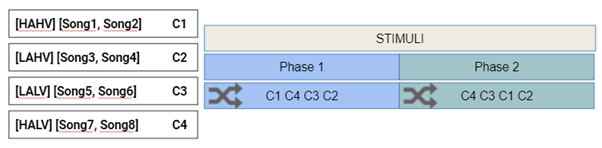
\includegraphics[width=12cm]{img/methods/inversion_criterion.png}
\centering
\caption{Pseudo randomization scheme. Participants listen to all songs twice, in both conditions, during the two parts of the experiment.} \label{fig_inversion_criterion}
\end{figure}

This approach also reduces the familiarity effect caused by listening twice to the same song in a short span of time and mitigates cases of extreme emotional fluctuation within each trial, for example if a very sad song would be followed by a very happy song and then again another sad song. This emotional fluctuation phenomenon cannot be fully eliminated, but it is statistically balanced by the pseudo-randomization of the order in which the classes are presented. 

\subsection{Equipment}
\label{sec:equipment}
During the pilot test some technical issues with the Melomind Q+ forced the use of the standard Melomind (Fig. \ref{fig_melomind}) in frontal setup using electrodes placed over [AF3 AF4] positions of the 10-20 system, thus reducing the amount of recording electrodes from 4 to 2 and requiring to adapt accordingly the entire research. The Melomind was connected via USB cable to a laptop through a TriggerBox and via Bluetooth to a smartphone to remotely control the start and end of the acquisition with  the proprietary Acquisier app developed by myBrainTechnologies. An Empatica E4  wristband was used to collect bio signals from the non-dominant wrist of the participant, namely: \ac{BVP}, body temperature, \ac{HR} and \ac{EDA} (Fig. \ref{fig_empatica}). 

\begin{figure}[h!]
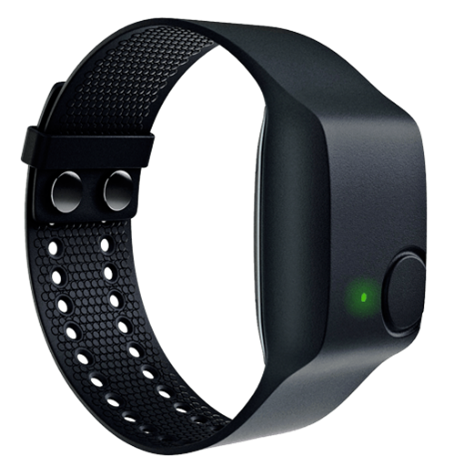
\includegraphics[width=6cm]{img/methods/empaticaE4.png}
\centering
\caption{EmpaticaE4, a wearable device that can record physiological data in real-time.} \label{fig_empatica}
\end{figure}

The Empatica E4 was connected to an Android tablet running the Empatica application, so the researcher could monitor in real-time the data collection. The \ac{EA} app was entirely developed as a set of automated routines in Psychopy, including trainings for the task, synchronization of the triggers with each experimental event and instructions for the users. The timers of each routine were calibrated during the pilot to allow even slower readers to follow up. 

\begin{figure}[h!]
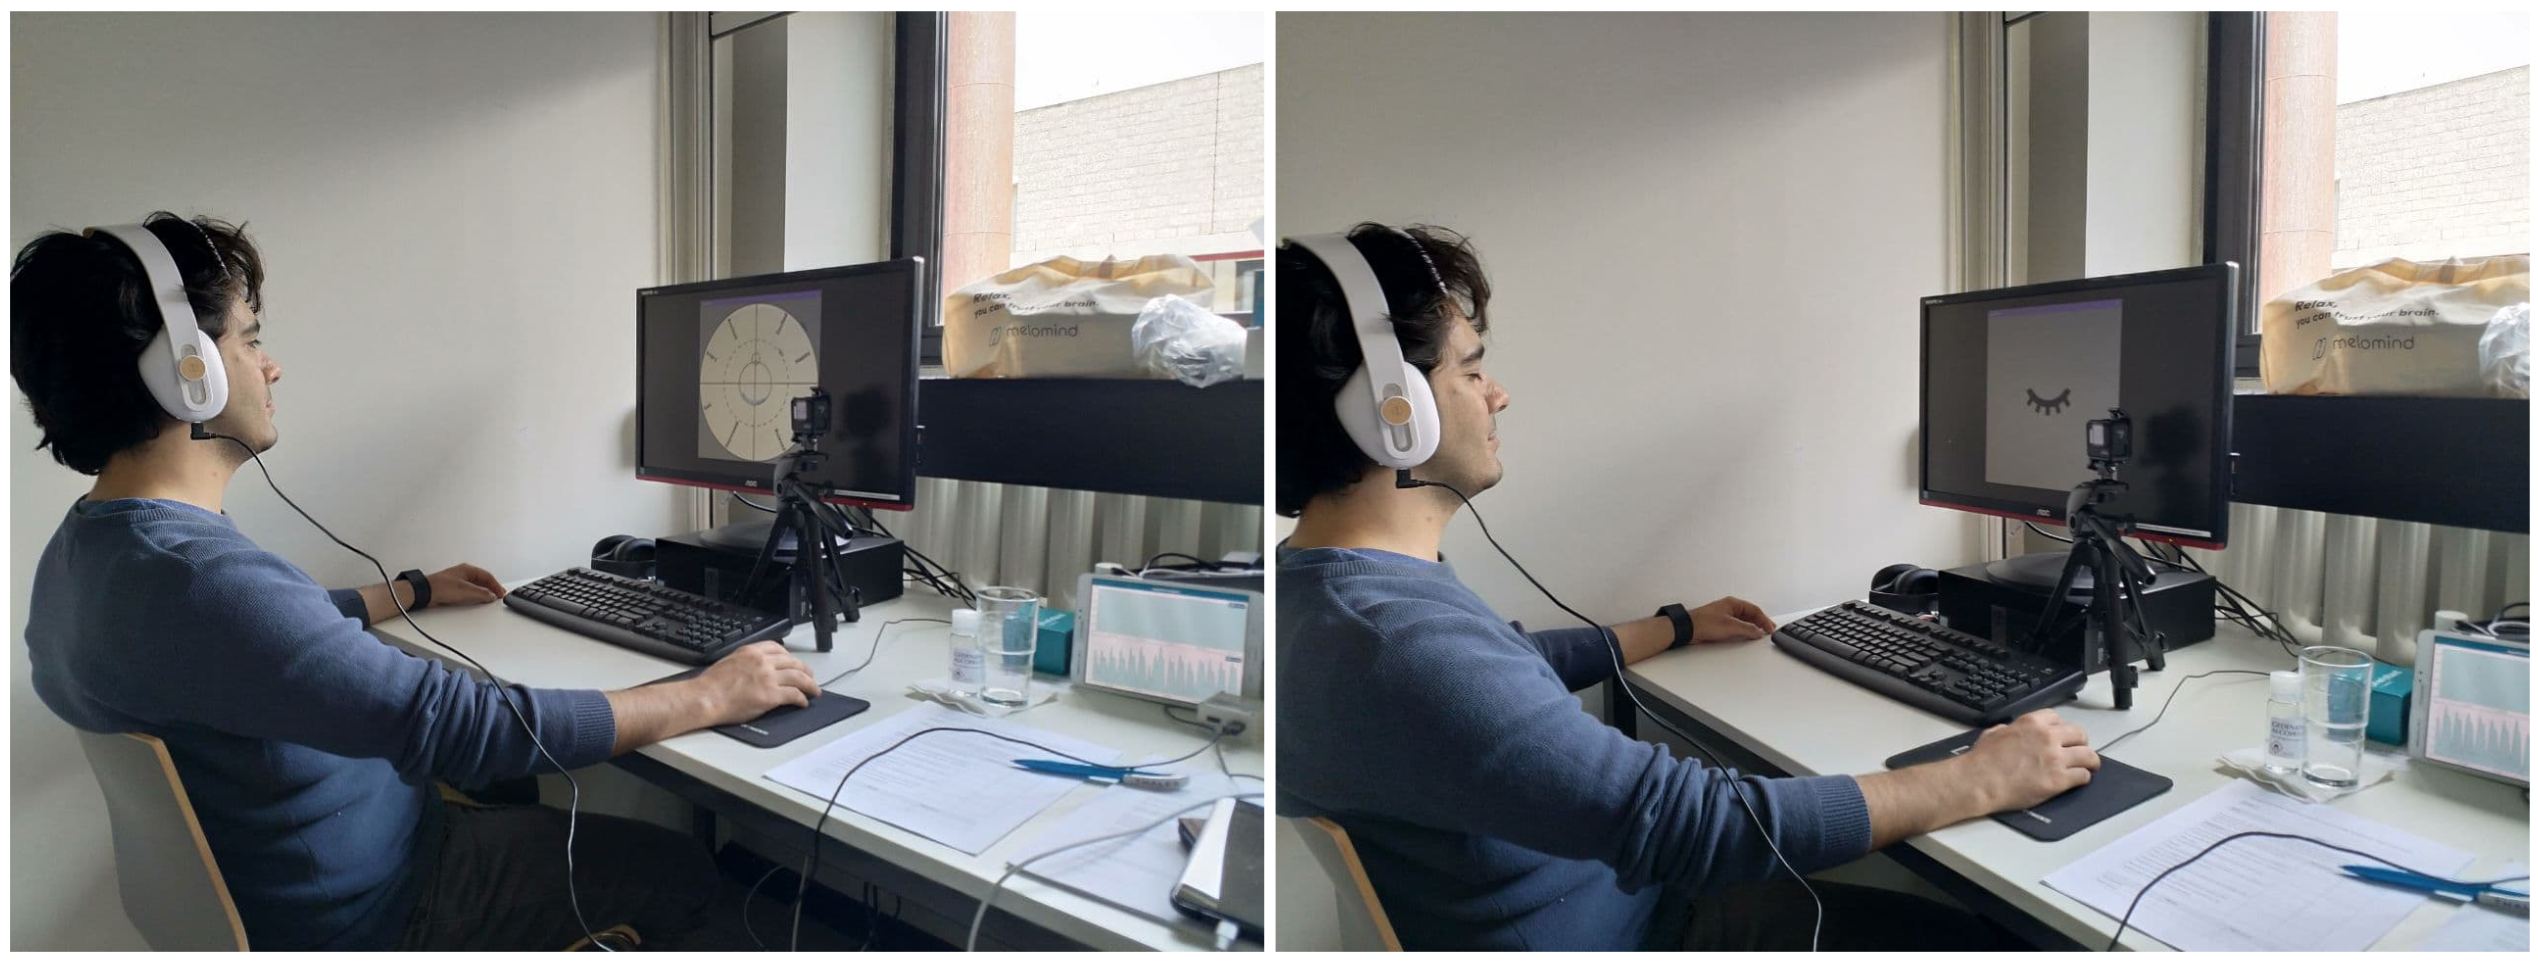
\includegraphics[width=12cm]{img/methods/experimental_setup.png}
\centering
\caption{Experimental setup with Melomind, Empatica E4 and GoProH7. The EA app is running on the monitor, while a participant is annotating emotions using the mouse (on the left) and then following instructions for the next task (on the right).} \label{fig_experimental_setup}
\end{figure}

The participants could interact with the experimental application through an external monitor connected to the researcher’s laptop and an agnostic mouse, although all participants decided to use the right hand. Finally, all the sessions were recorded with a GoPro Hero 7 to monitor accidental events and eventually support the emotion recognition task through facial expressions in a later study. An example of setup for the experiment can be see in Fig. \ref{fig_experimental_setup}. 



\subsection{Procedure}
\label{sec:procedure}
The experiment was conducted in a controlled environment made available by BMS lab at the University of Twente, with a strict protocol for sanitizing the equipment between each session, no direct skin-contact with the researcher during the setup, opening of the air flows every 10-15 minutes and at least 1.5 meters of distance with the researcher during the experimental task.

\begin{figure}[h!]
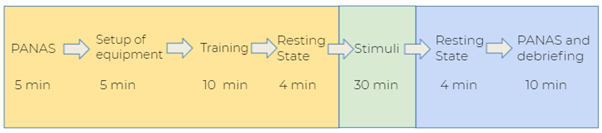
\includegraphics[width=10cm]{img/methods/exp_procedure.png}
\centering
\caption{Scheme of the experimental procedure, estimated to last ~75 minutes.} \label{fig_exp_procedure}
\end{figure}

Upon their arrival, participants were invited to sanitize their hands, to read and sign the informed consent form and then to fill a PANAS questionnaire \cite{watson_development_nodate} as part of myBrainTechnologies standard protocol for experimentation. The PANAS is used to measure the change in positive and negative affects in a specific span of time, from a few minutes up to a few weeks. In this case the span of time is the length of the experiment and researchers at myBrainTechnologies use these questionnaires to evaluate their experimental protocols and eventually support some evidences in their analyses. After the questionnaire, they could start the training session divided into three parts for a total of 10 minutes, without recording any \ac{EEG}. The first part gave some introduction and background about the Valence-Arousal model and allowed them to get some confidence with the annotation GUI. The second part proposed a mix of 4 music excerpts, one for each Valence-Arousal class, and asked them to annotate in real time with the emotions they were feeling. Finally, the third part was a complete simulation of an experimental trial, including instructions, white noises, both listening conditions and ratings. After the training, participants were asked to fit again the device on their head, then the researcher re-positioned the reference and recording electrodes to obtain the best possible quality signal using the \ac{QC} tool of the Acquisier app. The Empatica E4 was then fit on their wrist to allow a precise calculation of heart rate, and finally the Melomind was connected to the laptop through the TriggerBox. Participants were also advised to avoid sudden head movements. Before starting the session, their resting state baseline was recorded, 2 minutes in \ac{EO} condition and 2 minutes in \ac{EC} condition. When they were ready, they could start the session and follow the automated instructions, with the order of conditions determined by their assigned group. Halfway through the session they could take a 5-minute break, look away from the screen and drink some water, but they were not allowed to remove the equipment. After completing the second part of the session, another resting state was recorded with the same settings of the previous one, and then they filled the second PANAS questionnaire. The resting state recordings are also part of the standard myBrainTechnologies protocol to compare the mental changes in the resting states after an experiment and to be used as baseline during \ac{EEG} analysis. For this study only the resting state in the \ac{EC} condition prior to the experimental task was eventually used as recording baseline. At the end of the session all participants were asked to fill a feedback form to briefly evaluate the comfort of the experience, the clarity of the instructions and GUI, any difficulty in the annotation task and to report some behavioral preferences during music listening. Finally, they were debriefed on the purpose of the experiment and dismissed. The total length of the session was of 75 minutes on average, with a maximum of 90 minutes in some cases where the calibration of the equipment was not satisfactory, and the participants were then compensated for their participation.

\section{Data analysis}
\label{sec:data_analysis}
\subsection{Data preparation}
\label{sec:data_preparation}
The first step in the analysis process was to reorganize each participant’s dataset in a systematic collection that could be programmatically parsed. Due to the pseudo-randomization of the classes and the two different conditions, all trials, white noises, and resting states were flagged using an encoded label through the TriggerBox during the experimental phase. The labels were sent using timed events by the \ac{EA} app with a precision in the order of milliseconds. The resulting dictionary of events was used to split the \ac{EEG} recording and extract trials, white noises, and resting states. Each trial was associated with the appropriate label in the format "condition/class\_*\_*" , where condition could be a value between “EO” and “EC” to represent the recording condition, the first * could be a number in the range [1-4] to represent the valence-arousal  class, and the second * a letter between “A” or “B” to represent the order of presentation of a song within each trial. For example, "EO/class\_2\_A" represents the part A of a trial using music from the LAHV class and recording in \ac{EO} condition. In addition, for each \ac{EEG} segment, all the \ac{QC} labels were saved for later use in the preprocessing pipeline (see Chapter \ref{sec:automated_pipeline}). Then another dictionary containing the order of presentation of the classes was used to associate the metadata saved by the \ac{EA} app, namely the valence-arousal annotations and the familiarity/liking scores for each song, to the respective entry in the newly organized dataset. During the experiment sessions, some rare bugs in the recording application caused brief interruptions in the recording or the failure to register triggered events. For this reason, a total of 6 participants who had missing parts in their \ac{EEG} recordings or did not have the dictionary of events were excluded for further analysis. Their data could still be utilized in future studies by synchronizing the splitting functions with the timestamps saved in the metadata, but because of the time cost, it was decided to exclude them for the current research.

\subsection{Automated Pre-processing Pipeline}
\label{sec:automated_pipeline}
Given the goal of estimating the performances of a real-time oriented model, the pre-processing of the data had to consist of a lightweight and automated process that could be integrated in an application at some point. Consequently, more run-in tools like EEGLab and PREP \cite{bigdely-shamlo_prep_2015}, both based on the MATLAB programming language and very popular for offline analysis, were discarded in favor for more real-time oriented tools. Therefore, the \ac{AuPP} was implemented as a combination functions of the open-source Python library MNE\footnote{https://mne.tools/stable/index.html}  and the \ac{SPT} from myBrainTechnologies, a closed-source library that is more suitable to handle the proprietary data format of Melomind. After loading each participant’s prepared dataset, the \ac{AuPP} splits the signal in time windows of 5 seconds, removes the DC offset, applies a notch filter to remove power-line noise in the 50Hz and the 100Hz frequency bands, then applies a band-pass filter in the range 0.1Hz - 30Hz to remove slow and possibly large amplitude drifts and some movement artifacts outside of the frequency bands of interest (Fig. 22). Unfortunately, this light preprocessing is not suitable to remove most of the muscular artifacts, especially those generated by ocular movements that are frequently present in the frontal electrodes. In addition, having two electrodes hinders artifact detection using more sophisticated signal processing algorithms like \ac{ICA} and \ac{PCA}, that require a higher number of electrodes to effectively separate the signal in components and identify artifacts. To deal with artifacts, the \ac{AuPP} features two methods that can be used independently or in conjunction.

\begin{figure}[h!]
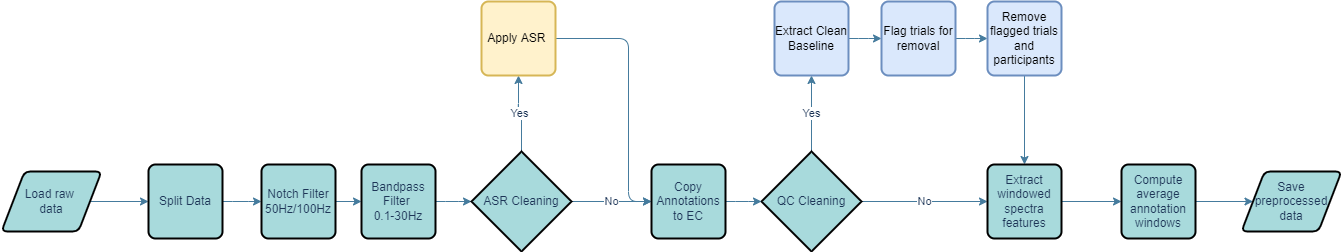
\includegraphics[width=15cm]{img/methods/preprocessing_pipeline.png}
\centering
\caption{Flowchart representing the preprocessing steps of the AuPP.} \label{fig_prep_pipeline}
\end{figure}

The first one is  \ac{ASR}, available in the open-source MEEGkit\footnote{https://nbara.github.io/python-meegkit/index.html}  library, that automatically tries to clean the signal by removing transient and large-amplitude artefacts. The second one is a custom method called \ac{QIRem}, implemented for this study, and based on the \ac{QC} proprietary classification-based method developed by myBrainTechnologies. The \ac{QC} algorithm has been developed to support researchers in real-time visual assessment of the quality of the signal \cite{grosselin_quality_2019}, and for each second of recording it assigns a label representing the quality of the signal as follows:
\begin{itemize}
\item 	Low Quality: LOW-Q = -1 and 0. 
\item 	Medium Quality with muscular artefacts: MED-MUSC = 0.25. 
\item 	Medium Quality: MED-Q = 0.5. 
\item     High Quality: HIGH-Q = 1.
\end{itemize}

The \ac{QIRem} method takes the \ac{QC} labels and redistribute them on a simpler scale from 0 to 1, where 0 corresponds to LOW-Q, 0.5 corresponds to MED-MUSC-Q and MED-Q and 1 corresponds to HIGH-Q, and then for each 5 seconds time window it calculates an average of the \ac{QC} labels.

\begin{figure}[h!]
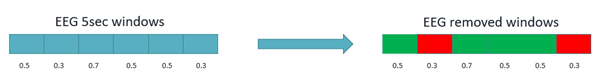
\includegraphics[width=15cm]{img/methods/qirem_example.png}
\centering
\caption{Example of how QIRem flags bad segments flagged for removal.} \label{fig_qirem_example}
\end{figure}

If the average is below a specified \emph{threshold} parameter, the EEG split is removed from the dataset (Fig. \ref{fig_qirem_example}). After removing all the contaminated splits if the dataset has lost more than the percentage of data  amount specified by the \emph{allowed loss} parameter, the entire participant’s dataset is flagged for exclusion from the analysis. During the tuning of the \ac{AuPP}, it was finally decided to avoid using \ac{ASR} to clean the signal, because it requires to be trained on a sufficiently clean segment of signal, unfortunately not guaranteed to exist for all subjects, and most often resulted in very aggressive cleaning that would flatten the signal (Fig. \ref{fig_asr_example}).

\begin{figure}[h!]
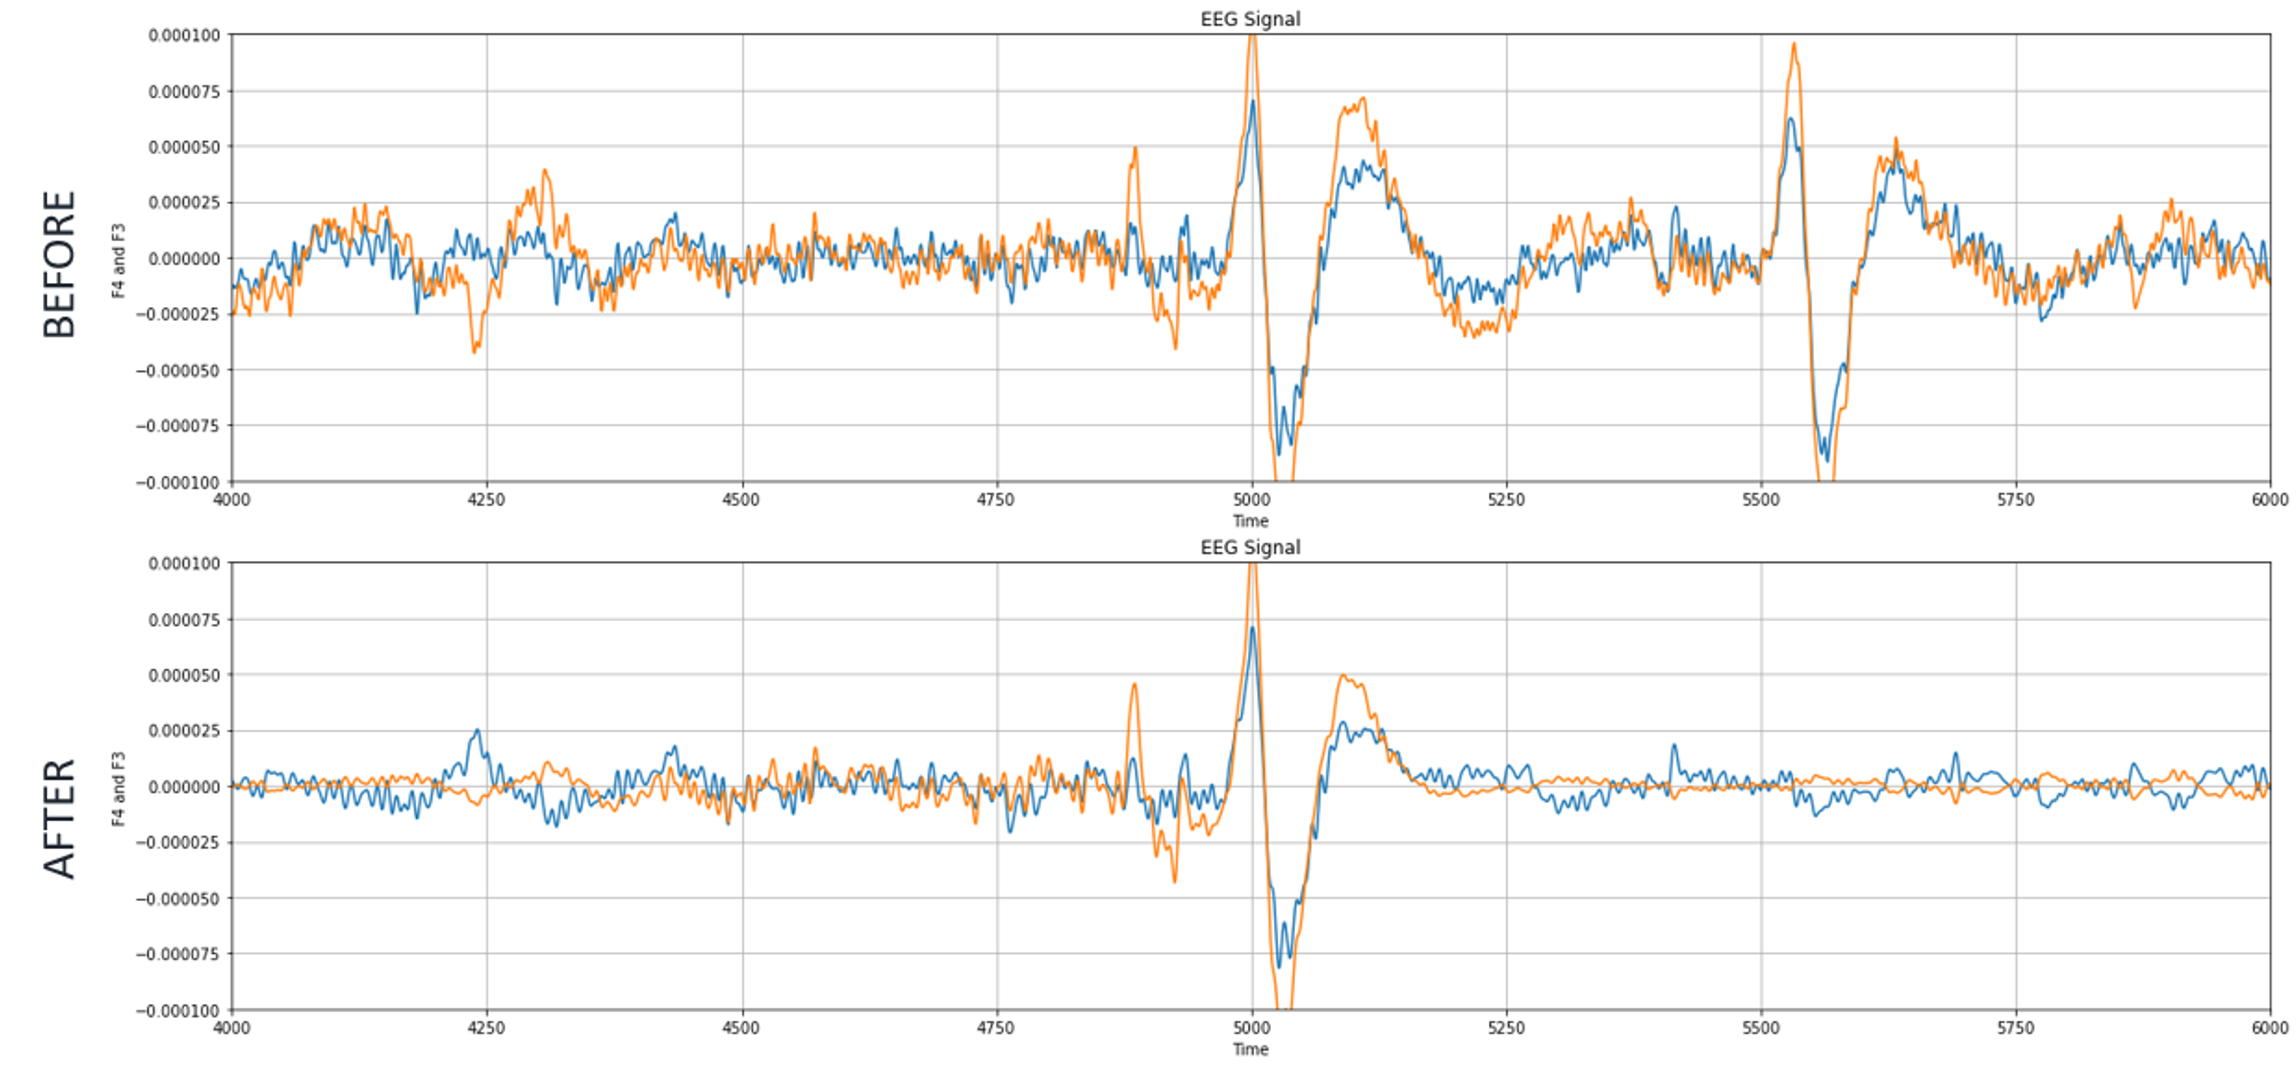
\includegraphics[width=15cm]{img/methods/asr_example.png}
\centering
\caption{Examples of the effects of ASR on the signal.} \label{fig_asr_example}
\end{figure}

The \ac{QIRem} method was setup with \emph{threshold} set to 0.5 and \emph{allowed loss} set to 0.25, meaning that the average quality of each time window had to be equal or above 0.5 in the simplified scale and that at most 25\% of data could be pruned before flagging the entire dataset for exclusion. With the current configuration, 10 participants were excluded from further analysis, hence the reason why the threshold was kept around medium quality (0.5), allowing some artefacts to persist in the data. This approach is a compromise choice that carries three main problems that must be addressed in future studies:
\begin{itemize}
\item 	Very aggressive: bad quality data are not cleaned, but removed instead, possibly losing meaningful information and control over the distribution of the class labels.
\item 	Exclusive: 10 out of 39 participants were excluded from analysis, which summed up to those excluded for other reasons is more than 1/3 of the entire experimental dataset.
\item 	Not Optimized: one limitation of the Quality Checker algorithm is that it was trained for the consumer use on Melomind with electrodes placed on the parietal area of the scalp (P3, P4), so while able to discriminate good and bad quality segments of signal, it has no specific label for ocular artifacts. An upgraded version is under the work to provide classification of these artifacts.
\end{itemize}

\subsection{Features Computation}
\label{sec:features_computation}
To compute the spectral features, the \ac{PSD} of each 5 seconds window of the \ac{EEG} signal was extracted and filtered for theta, alpha and beta frequency band using the \ac{SPT} wrapper for the \ac{FFT}. Before computing features, the time-frequency power was normalized using the decibel conversion method as described by M. X. Cohen \cite{cohen_analyzing_2014}. Time-frequency power follows a 1/f shape function, meaning that frequency spectrum tends to show decreasing power at increasing frequencies, \ac{EEG} included. Consequently, there are 4 main limitations:


\begin{enumerate}
\item 	Difficulty in making power comparisons across such bands. Raw power values change in scale as a function of frequency, meaning that lower frequencies (Delta, Theta) will show larger effect than higher frequencies in terms of overall magnitude.
\item 	Aggregation of subject-independent effects will not yield good results because of differences influenced by skill thickness, sulcal anatomy, cortical surface, recording environment or other internal and external factors.
\item 	Task-related changes in power can be tainted by background activity, particularly for frequencies that tend to have higher power, especially during baseline periods (Alpha).
\item 	Raw powers do not follow a normal distribution because they cannot be negative, and they are strongly positively distorted.
\end{enumerate}
Using decibel conversion, which is an expression of power as the ratio between strength of one signal (frequency-band-specific-power) and the strength of another signal (a baseline level of power in the same frequency band).
\[dB_{tf} = 10log10 \left(\frac{activity_{tf}}{\overline{baseline_{tf}}} \right)\]
The scale and interpretation of frequency-band-specific power becomes the change in power relative to the baseline. Any frequency-band-specific activity constant over time will be removed, including background activity. As a baseline for normalization, the resting state in the \ac{EC} condition was used, to prevent ocular artifacts from contaminating the trials. The baseline resting state, previously divided in 5 seconds time window, and pre-processed together with the other trials, was pruned from low quality segments using the \ac{QIRem} function and then averaged across all the time windows, for each channel. The main advantages obtainable by normalizing the date are the following: 

\begin{itemize}
\item 	All power data are re-scaled to the same scale and thus can be compared visually and statistically
\item 	Normalization computed in respect to a pre-trial baseline enables to disentangle time-frequency dynamics from background or task-unrelated dynamics
\item 	All power results are in a common and easily numerically interpretable metrics
\item 	Parametric statistical analysis is appropriated to use (for baseline-normalized power data normally distributed) and quantitative group-level analyses and integration with other data (behavioral performance, questionnaires) is facilitated. 
\item 
\end{itemize}
The features extracted include the neuromarkers described in Chapter \ref{chap:background} and additional properties of the power spectrum that could strengthen the models’ ability to discriminate emotional dimensions. It was decided in a later stage to use these properties of the raw signal because they could be conveniently extracted using the \ac{SPT} and potentially make up for information lost during the computation of the neuromarkers.
For each 5s time window the following measurements were computed and stored, for a total of 40 features among the two channels to be used in classification:
\begin{enumerate}
\item 	Normalized power in Theta, Alpha and Beta frequency bands
\item 	Approach-Withdrawal Index 
\item 	Frontal-Midline Theta Index
\item 	Spectral Asymmetry Indexes
\item 	Skewness of the power in Theta, Alpha and Beta frequency bands
\item 	Kurtosis of the power in Theta, Alpha and Beta frequency bands
\item     Standard deviation of the power in Theta, Alpha and Beta frequency bands
\item 	Ratio of the power in Theta, Alpha and Beta frequency bands
\item 	Relative spectral difference of the power in Theta, Alpha and Beta frequency bands
\end{enumerate}


\begin{figure}[h!]
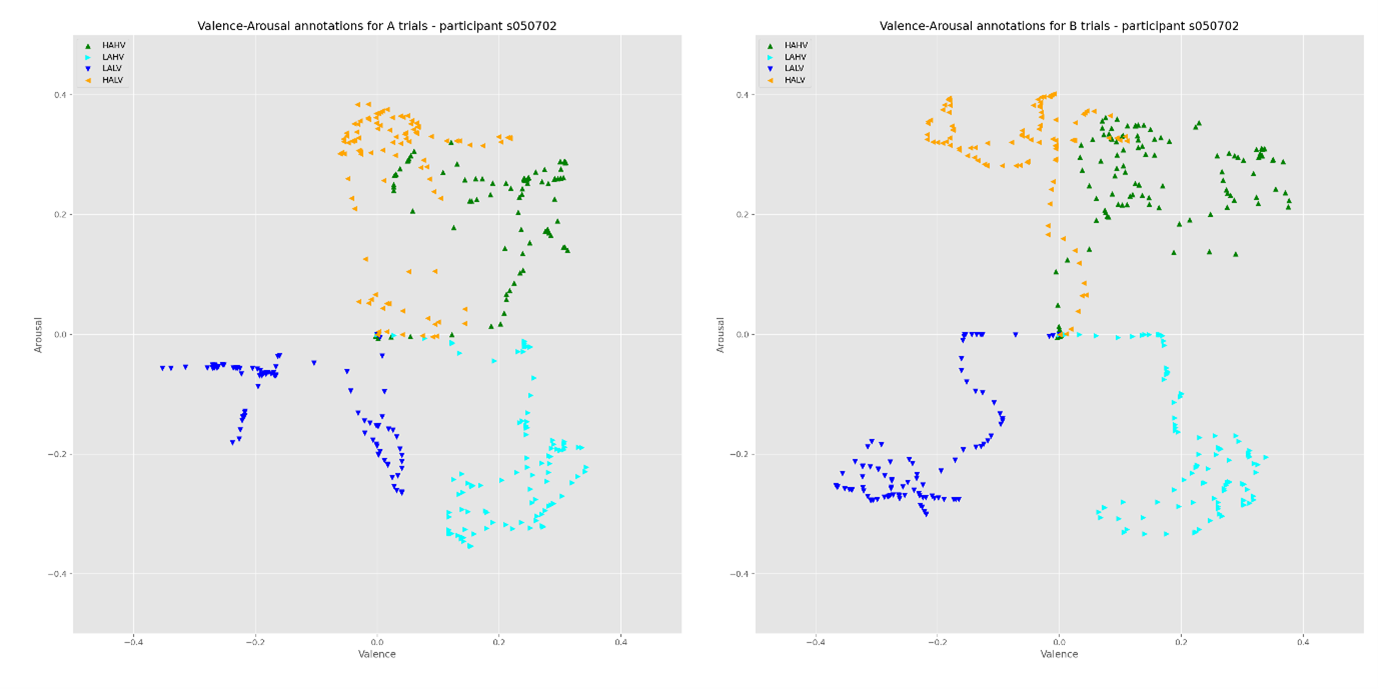
\includegraphics[width=15cm]{img/methods/example_avg_annotations.png}
\centering
\caption{Example of annotations of a single participant for all trials. The labels are color coded according to the pre-labelled VA class of each song.} \label{fig_avg_annotations}
\end{figure}

Finally, the raw VA annotations (Fig. \ref{fig_avg_annotations}) were averaged for each time-window and then converted into positive labels whether the average was positive, or negative labels otherwise. Consequentially, each time window was labelled twice: first as HA or LA (High/Low Arousal), and then as HV or LV (High/Low Valence). The union of the two labels generates one of the class labels of the Valence-Arousal quadrant that represent the emotion elicited in that specific time window, according to the notation proposed by Koelstra et al. \cite{koelstra_deap_2012} (see Chapter \ref{sec:stimuli}). In some studies, the notation for valence is defined as PV and NV (Positive/Negative Valence), which is better aligned with the etymology of positive and negative emotions. The labels were also copied for each song from the \ac{EO} listening condition to the respective \ac{EC} listening condition.

\subsection{Classification}
\label{sec:classification}
The classification pipeline was implemented using the open-source Python library Scikit-Learn\footnote{https://scikit-learn.org/stable/index.html}. Multiple experiments were conducted with two supervised learning models, \ac{SVM} and \ac{MLP}. These models are a popular choice for the Emotion-Recognition task thanks to their relative simplicity yet their superior capacity to handle not linearly separable data compared to statistical linear models (see Chapter \ref{sec:classification_emotions}). The \ac{SVM} architecture was defined using RBF kernel, that usually grants better accuracy, and it is relatively easy to calibrate, and decision function one-vs-one for binary classification and one-vs-rest for multi-class classification. The architecture for \ac{MLP} was based on the LBFGS optimizer, a quasi-Newtonian method, that is more suitable for small datasets and can converge faster with better perforances and \emph{ReLU} was chosen over \emph{TanH} as activation function because it reduces the impact of vanishing gradients, even if no substantial difference was observed while testing both. The problem has been set as a separate binary classification of Arousal and Valence using a subject-dependent strategy, similarly to most related studies. As explained in the Section \ref{sec:intermediate_experiments}, during the intermediate experiments the listening condition did not reveal significant differences in the classification performances, therefore all the trials of each subject were later unified under a third condition named “EO\&EC” to take advantage of the greater amount of data-points. Then, from each subject dataset, a total of 40 previously computed features were loaded in the classification pipeline.
\begin{figure}[h!]
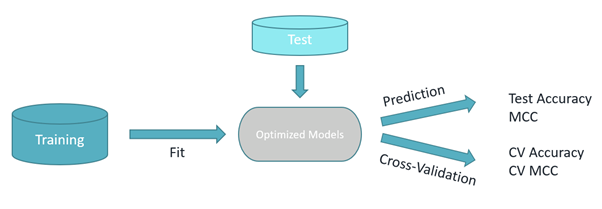
\includegraphics[width=12cm]{img/methods/data_split_strategy.png}
\centering
\caption{Approach used to compute Test Accuracy, MCC, CV Accuracy and CV MCC with separate splits of data.} \label{fig_data_split_strategy}
\end{figure}
To begin with, the data were split into a training dataset and a test dataset in 80:20 proportion and scaled using MaxAbsScaler, that re-scales the data to its maximum absolute value without shifting or centering it, thus preserving any sparsity.\ac{PCA} was used to identify the features contributing for the 95\% of the variability of the dataset and projecting them on a lower dimensional space, reducing the dimensionality to ~12 components and greatly reducing the overall computation time, often referred to as \emph{curse of dimensionality}. After applying \ac{PCA}, the training dataset was used to tune the best hyper-parameters each classifier, respectively \emph{C} and \emph{Gamma} for \ac{SVM} and \emph{Alpha} and \emph{Hidden Layer Sizes} for \ac{MLP}, using GridSearch with a K-Fold Cross-Validation strategy, k=5 (see Fig, \ref{fig_data_split_strategy}). Finally, the tuned classifiers were trained with K-Fold Cross Validation \ac{LOBO} for testing, and the relevant score metrics were collected.

\subsection{Intermediate experiments}
\label{sec:intermediate_experiments}
The classification problem was initially addressed as a binary classification problem for Arousal and Valence and then as a multi-class classification problem for Valence-Arousal. During the initial experimentation phase, these models were manually tuned and studied keeping the listening condition separated and then adding a third condition defined as EO\&EC, composed by data from both listening conditions joint together. To explore each condition and each type of model, a binary classifier for Arousal, a binary classifier for Valence and a multi-class classifier for Valence-Arousal were trained, following both subject-dependent and subject-independent strategy, for a total of 36 possible combinations. All the other hyper-parameters were initially manually tuned and kept identical for each classifier (see Appendix \ref{sec:appendix_A3.1}). The first full-scale experiment was launched with subject-dependent strategy and to reduce the dimensionality of the data, the 5 most relevant features were selected using forward \ac{SFS} with cross-validation to select the features most contributing to the variability of the data and using them to train each subject’s classifiers with cross-validated scores. Consequently, the selected features were ranked by adoption rate among all participants (see Appendix \ref{sec:appendix_A3.1}) and appointed as TOP5 features. It should be emphasized that this operation was computationally intensive and took several hours to complete, underlying the necessity for a better approach to envision a real-time application. Another subject-dependent experiment was run, this time using the same pre-selected TOP5 features for each participant, followed by a subject-independent experiment with the same configuration with cross-validation and \ac{LOSO}. The results of all experiments have been collected and averaged (see Appendix \ref{sec:appendix_A3.1}, \ref{sec:appendix_A3.2}, \ref{sec:appendix_A3.4}). A few observations were made that led to further investigation and the search for a better approach:
\begin{itemize}
\item 	\ac{EC} and \ac{EO} conditions did not show significant differences in performance, suggesting that the study could continue using just the EO\&EC condition, greatly reducing computation time and simplifying the analysis.
\item 	The multi-class classifiers for \ac{VA} reported the worst performances, thus was discarded to focus the efforts on optimizing the binary classifiers.
\item 	Many datasets were highly unbalanced in the distribution of the labels among the four \ac{VA} classes and both \ac{MLP} and \ac{SVM} struggled to discriminate positive and negative class, with \ac{SVM} always default guessing the majority class.
\item 	Subject-Independent performance always resulted very close and sometimes worse than default guessing the majority class.
\item 	Selecting the average TOP5 features among all participants is idealistically a good choice for a subject-independent strategy, but given the more promising subject-dependent results, this approach is at best losing data variability for some of the subjects and at worse using the least contributing features for some others.
\end{itemize}

Further investigation in the subjects labelling behavior and in the models’ predictions (see Appendix \ref{sec:appendix_A3.4}) led to the decision to optimize the strategy in function of subject-dependent classification.

\subsection{Unbalanced labelling}
\label{sec:unbalanced_labelling}
The stimuli were selected to elicit a wide as possible range of emotions to cover evenly the Valence-Arousal quadrants. However, when selecting music that has been pre-labelled with the average opinion of hundreds of annotators, there is always a possibility that part of the population disagrees. These subjects are not per se “bad annotators”, but their personal taste and perception lies outside of median. The distribution of labels across all subjects in Figure \ref{fig_labels_distribution} also reveals that positive classes are in general the most reported, with HAHV and LAHV taking absolute lead, and corresponding to emotions very common during the music listening experience: excitement, happiness, satisfaction, calm etc.

\begin{figure}[h!]
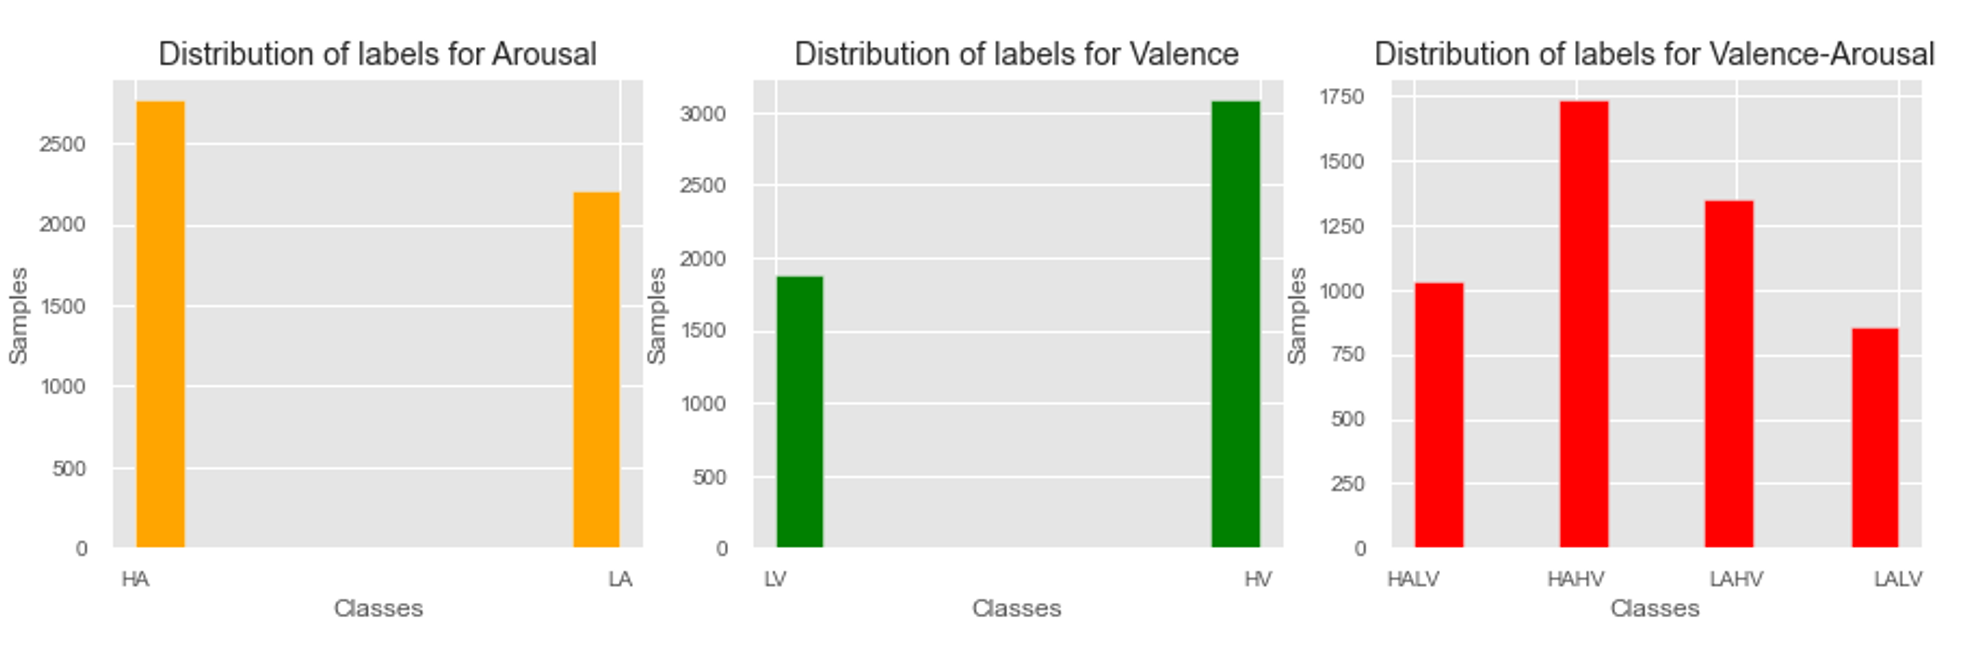
\includegraphics[width=12cm]{img/methods/labels_distribution.png}
\centering
\caption{Distribution of arousal, valence, and Valence-Arousal labels across all subjects.} \label{fig_labels_distribution}
\end{figure}

Furthermore, the personal perception of a subject can be heavily biased by external factors such as memories, genres preferences or unexpected events occurred over the day that are outside of the experiment control capabilities. In some cases, this led to very extreme distributions of data (Fig. \ref{fig_unbalanced_example}).

\begin{figure}[h!]
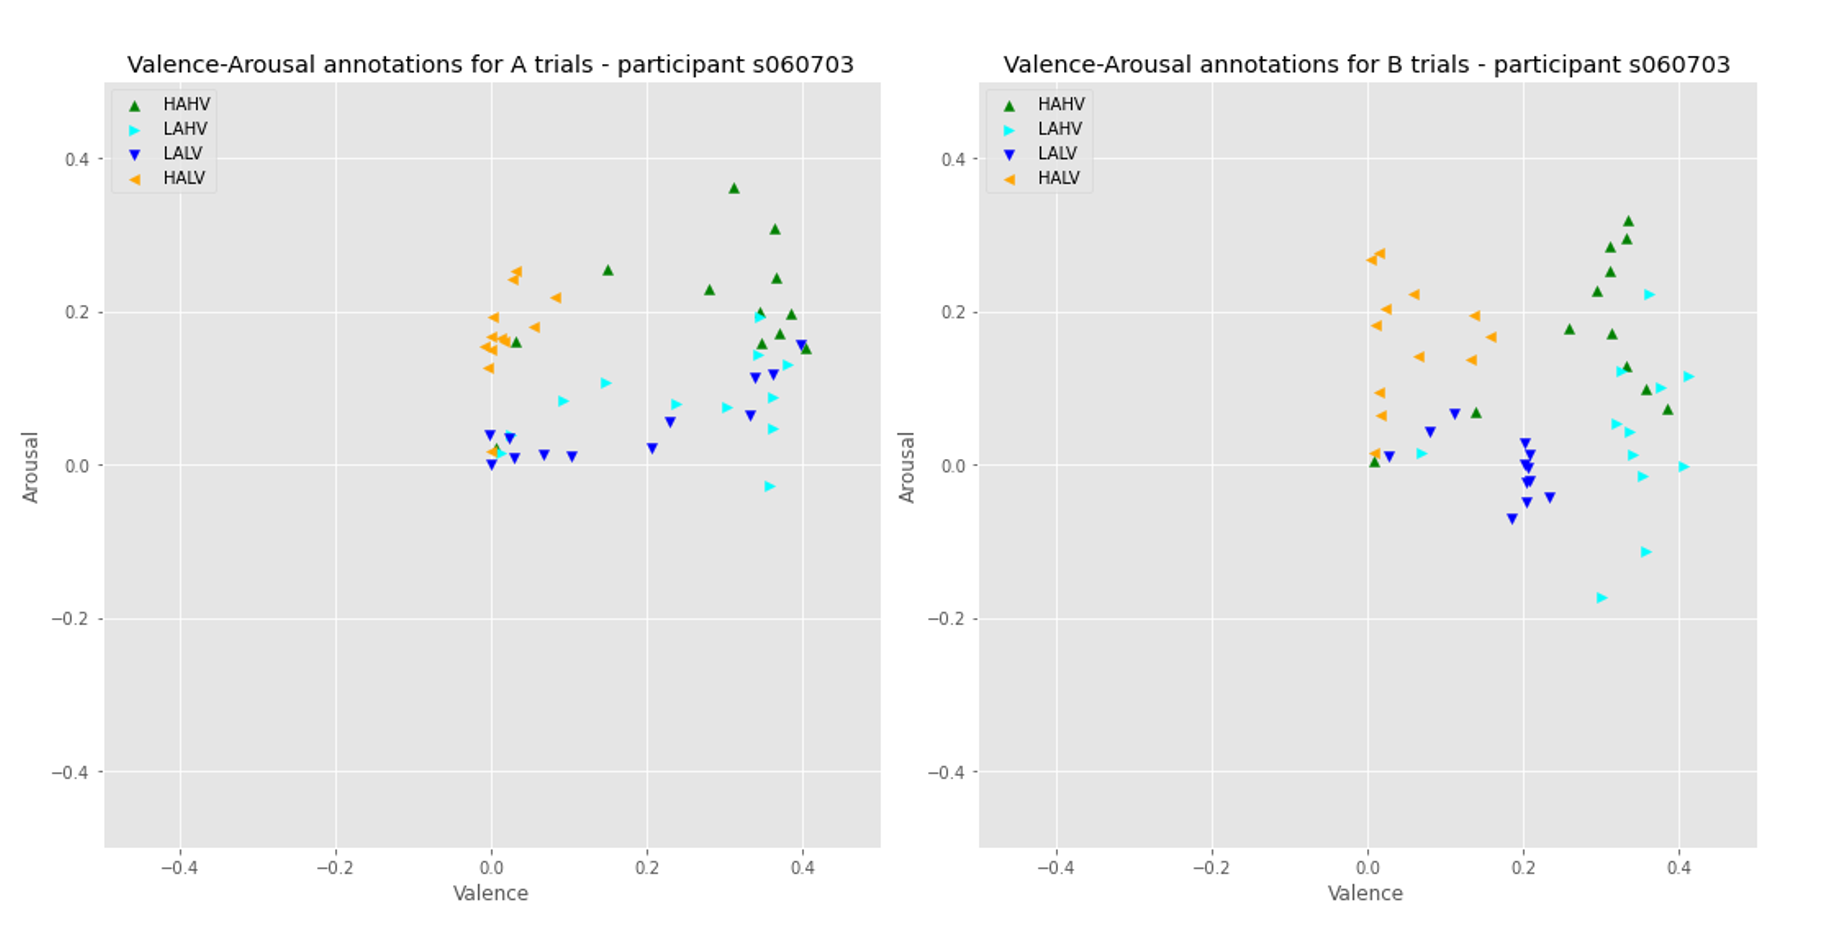
\includegraphics[width=12cm]{img/methods/unbalanced_example.png}
\centering
\caption{Annotations averaged over a 5 second window for a subject with unbalanced dataset. The labels are color coded according to the pre-labelled VA class of each song.} \label{fig_unbalanced_example}
\end{figure}

Although just a few data points of this subject lie in the negative spectrum of Arousal and Valence, the continuous annotations allow to capture them while discrete annotations at the end of each song might have ended up all in the HAHV class, thus hindering any classification. However, a classifier trained to obtain the maximum accuracy would always overfit and opt to classify the majority class, misleading the interpretation of its performances. 

\subsection{Optimizations}
\label{sec:optimizations}
All the problematics were addressed before proceeding with the final experiment. First, the dimensionality of the features was reduced using \ac{PCA} to select the 95\% most contributing components, greatly reducing the computational time and the risk of excluding meaningful features. Then \ac{MCC} \cite{matthews_comparison_1975} was introduced as scoring parameter to provide better interpretability of the accuracy scores. The \ac{MCC} is a correlation coefficient between the observed and predicted binary classification and is defined by the following formula: 
\[MCC = \frac{TP \times TN - FP  \times FN}{\sqrt{(TP + FP)(TP + FN)(TN+ FP)(TN + FN)}}\]
The \ac{MCC} value ranges between -1 and +1, where +1 represents a perfect prediction, 0 a random prediction and -1 and inverse prediction. Unlike the F1 score, that is the harmonic mean of precision and recall, the \ac{MCC} considers all the four quadrants of the confusion matrix of a prediction, making it a more reliable measure for the learning performances of a model for binary classification, even when the dataset is unbalanced \cite{chicco_advantages_2020}. The large number of factors that may hinder the Emotion-Recognition task are reflected in the large variability of the classification results across subjects and thus using solely the accuracy to measure the performances is not optimal and more studies \cite{thammasan_multimodal_2017, keelawat_comparative_2021} now relying on \ac{MCC} score’s reliability to explain the learning capabilities of their models. To optimize the models for the subject-dependent strategy, GridSearch was used with K-Fold Cross-Validation on the training split of each subject dataset to find the configuration that would yield the highest \ac{MCC} score (see Fig. \ref{fig_scheme_data_splitting}). 

\begin{figure}[h!]
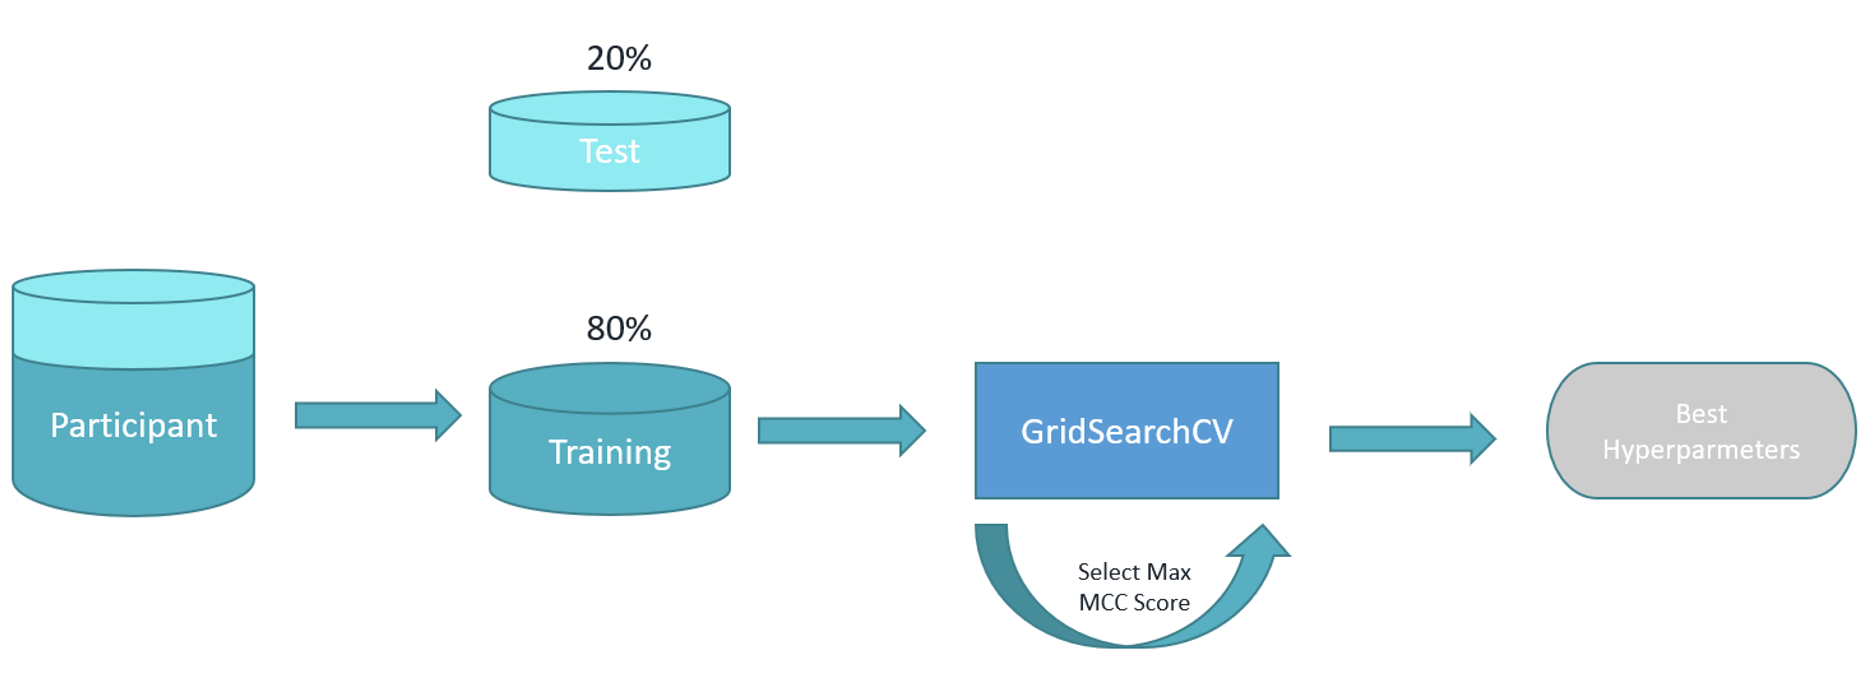
\includegraphics[width=12cm]{img/methods/scheme_data_splitting.png}
\centering
\caption{Scheme of data splitting strategy for cross-validated GridSearch optimization.} \label{fig_scheme_data_splitting}
\end{figure}

In addition, \ac{SVM} models were also initialized with the weights of each class based on the distribution of the labels. Currently there is a known limitation in the Scikit-learn library, as it does not seem to support custom loss functions to optimize scoring parameters other than accuracy, a missing feature reported by users of the library \cite{martin_stacked_nodate, noauthor_please_nodate}. Consequently, when feeding \ac{MCC} as scoring parameter, it only means that after optimizing accuracy for all possible configurations, the configuration with highest \ac{MCC} is selected. Two scoring strategies for GridSearch were tested in the experiment:
\begin{itemize}
\item 	Maximization of \ac{MCC} score, defined as “Max MCC” strategy
\item 	Maximization of Accuracy score, defined as “Max Accuracy” strategy
\end{itemize}
The results of the two scoring strategies are compared in the next section.


\section{Better learning or better accuracy}
\label{sec:better_learning_accuracy}
The purpose of this intermediate experiment was to compare the scoring strategies; however, it is important to underline that the loss function implemented in the scikit-learn library for GridSearch is chosen to optimize accuracy and only then the scoring parameter is used to select the best configuration. The results of subject-dependent arousal classifications are reported in Table 3, and they are not significantly different from the previous experiment. However, the highest consistent accuracy score using \ac{MLP} is 77\% with \ac{MCC} score of 0.53. Furthermore, it is possible to notice an increased number of negative \ac{MCC} and \ac{CV MCC} scores, and for \ac{MLP} the best performing models are not entirely consistent with the previous experiment.

\begin{table}[h!]
  \caption{Arousal classification results using Accuracy as scoring parameter for GridSearch. The 5 best performing models in terms of accuracy and MCC score are highlighted in blue, the models with MCC <= 0 and CV MCC <= 0 are highlighted in orange and yellow, respectively.}
  \label{tbl:arousal_max_acc_results}
  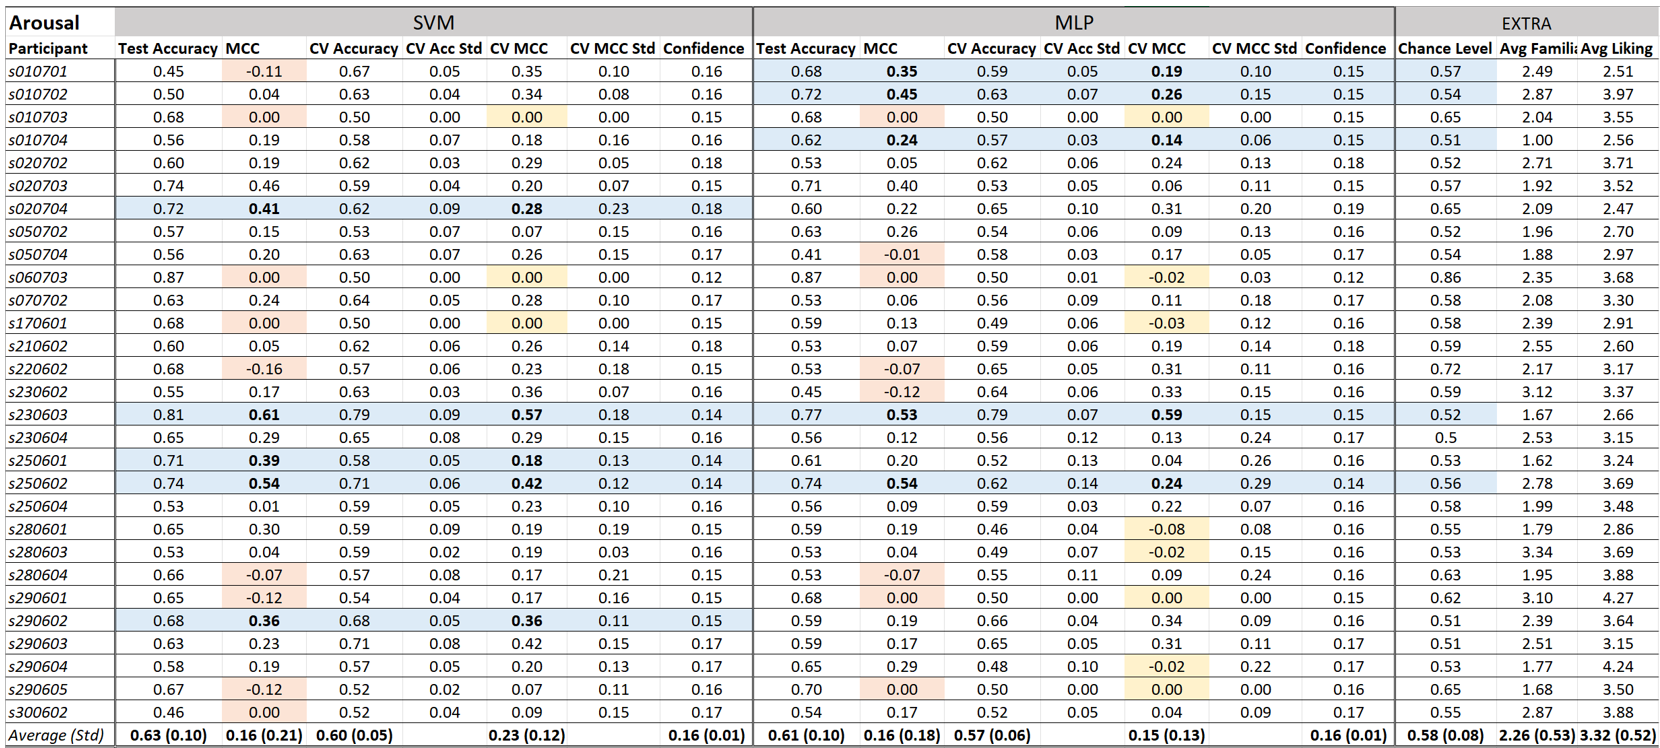
\includegraphics[width=\linewidth]{img/results/arousal_max_acc_results.png}
\end{table}

For valence classification the average test score is slightly higher for both \ac{SVM} and \ac{MLP}, but the highest accuracy score for \ac{MLP} reaches 90\% with \ac{MCC} score of 0.36. For \ac{SVM} the highest accuracy score is 80\% with \ac{MCC} score of 0.11. These highest accuracy scores are not consistent with the previous experiment and the relatively lower associated \ac{MCC} scores can be explained by the different scoring strategy.

\begin{table}[h!]
  \caption{Valence classification results using Accuracy as scoring parameter for GridSearch. The 5 best performing models in terms of accuracy and MCC score are highlighted in blue, the models with MCC <= 0 and CV MCC <= 0 are highlighted in orange and yellow, respectively.}
  \label{tbl:valence_max_acc_results}
  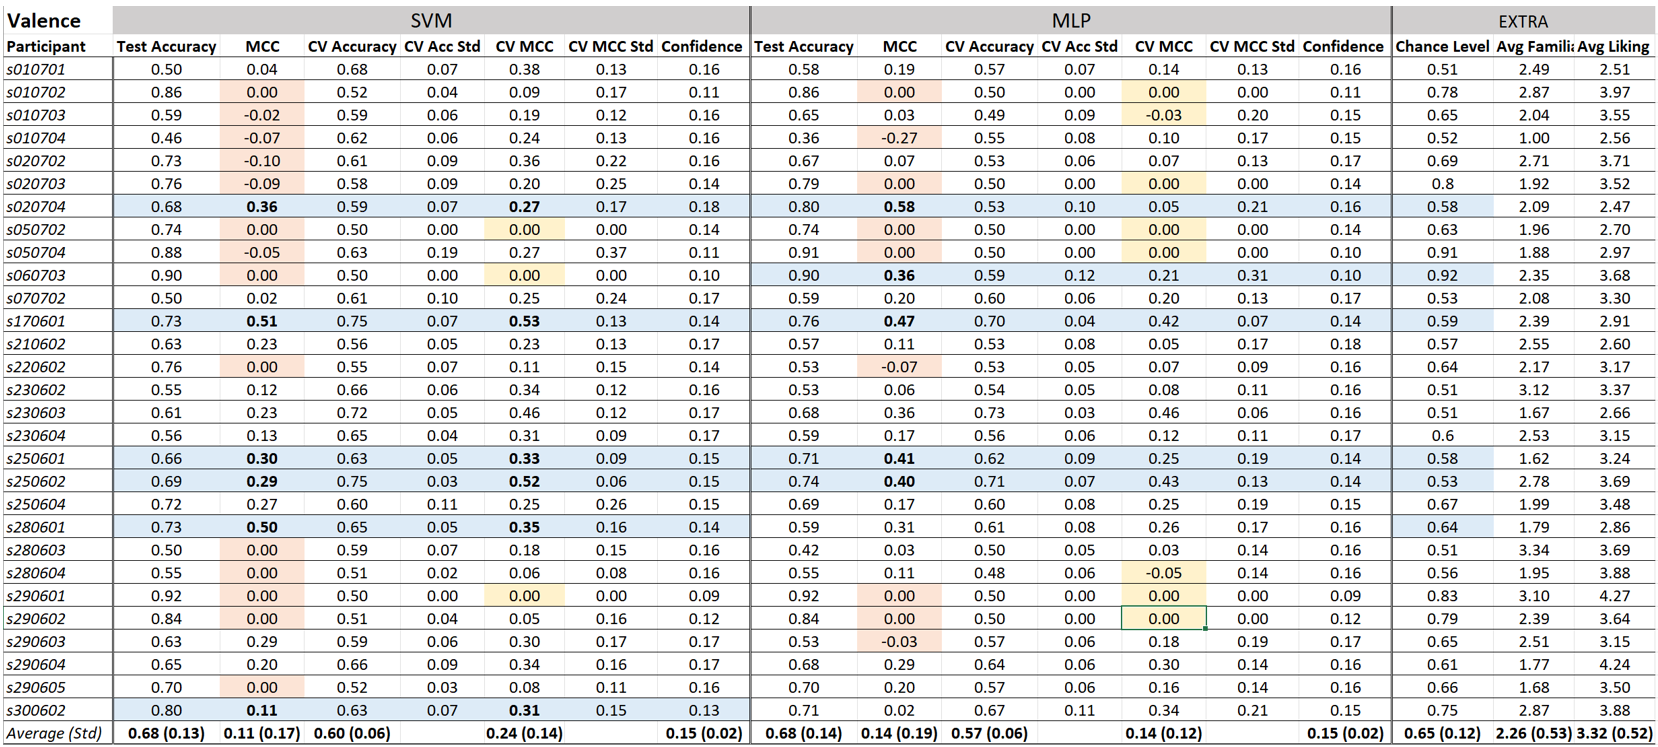
\includegraphics[width=\linewidth]{img/results/valence_max_acc_results.png}
\end{table}

Overall, it is also noticeable that an increased number of models is not learning, either because of over-fitting or under-fitting. This is particularly evident for arousal classification. This can be observed in the plots in Fig. \ref{fig:arousal_strategy_comparison} and Fig. \ref{fig:valence_strategy_comparison}, in which the number of models scoring 0 or less in \ac{MCC} and \ac{CV MCC} scores is compared between both strategies, for arousal and valence respectively.

\begin{figure}[h!]
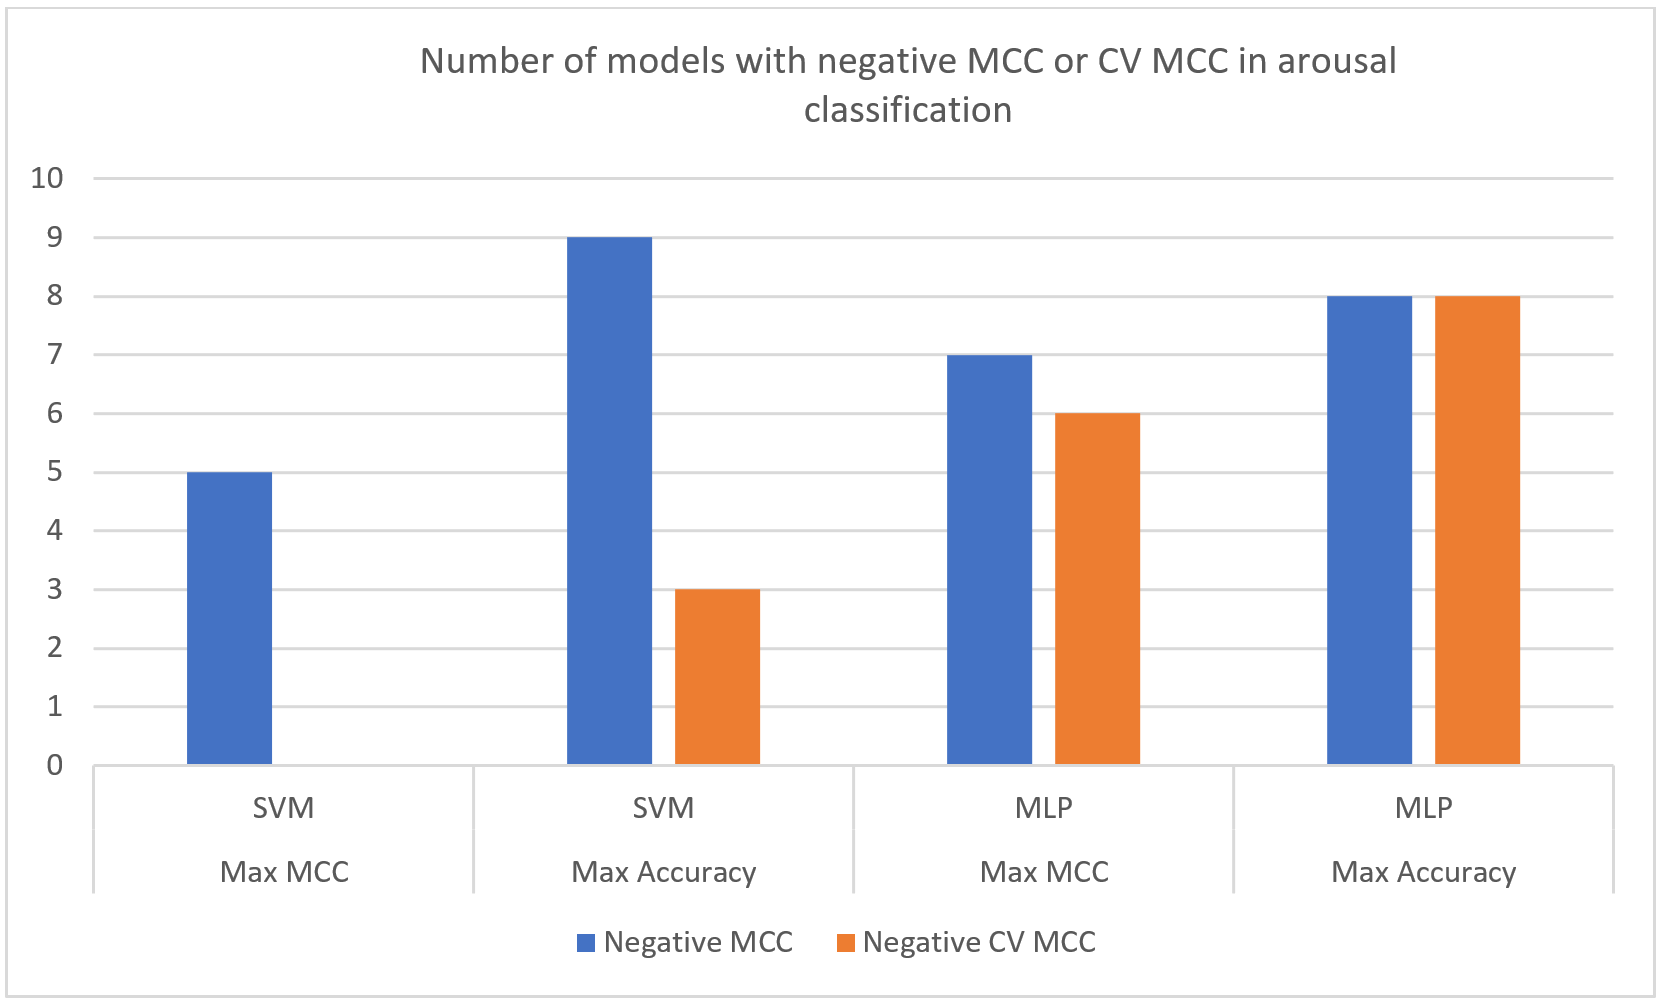
\includegraphics[width=12cm]{img/results/arousal_strategy_comparison.png}
\centering
\caption{Comparison between optimization strategies of negative MCC and CV MCC scores counts for arousal classification.} \label{fig:arousal_strategy_comparison}
\end{figure}

For arousal classification the difference between Max MCC strategy is evident and significant for \ac{SVM} classifiers, and there is increasing trend between Max MCC strategy and Max Accuracy Strategy. In valence classification the difference is less remarkable, but the same increasing trend between the two strategies is present.

\begin{figure}[h!]
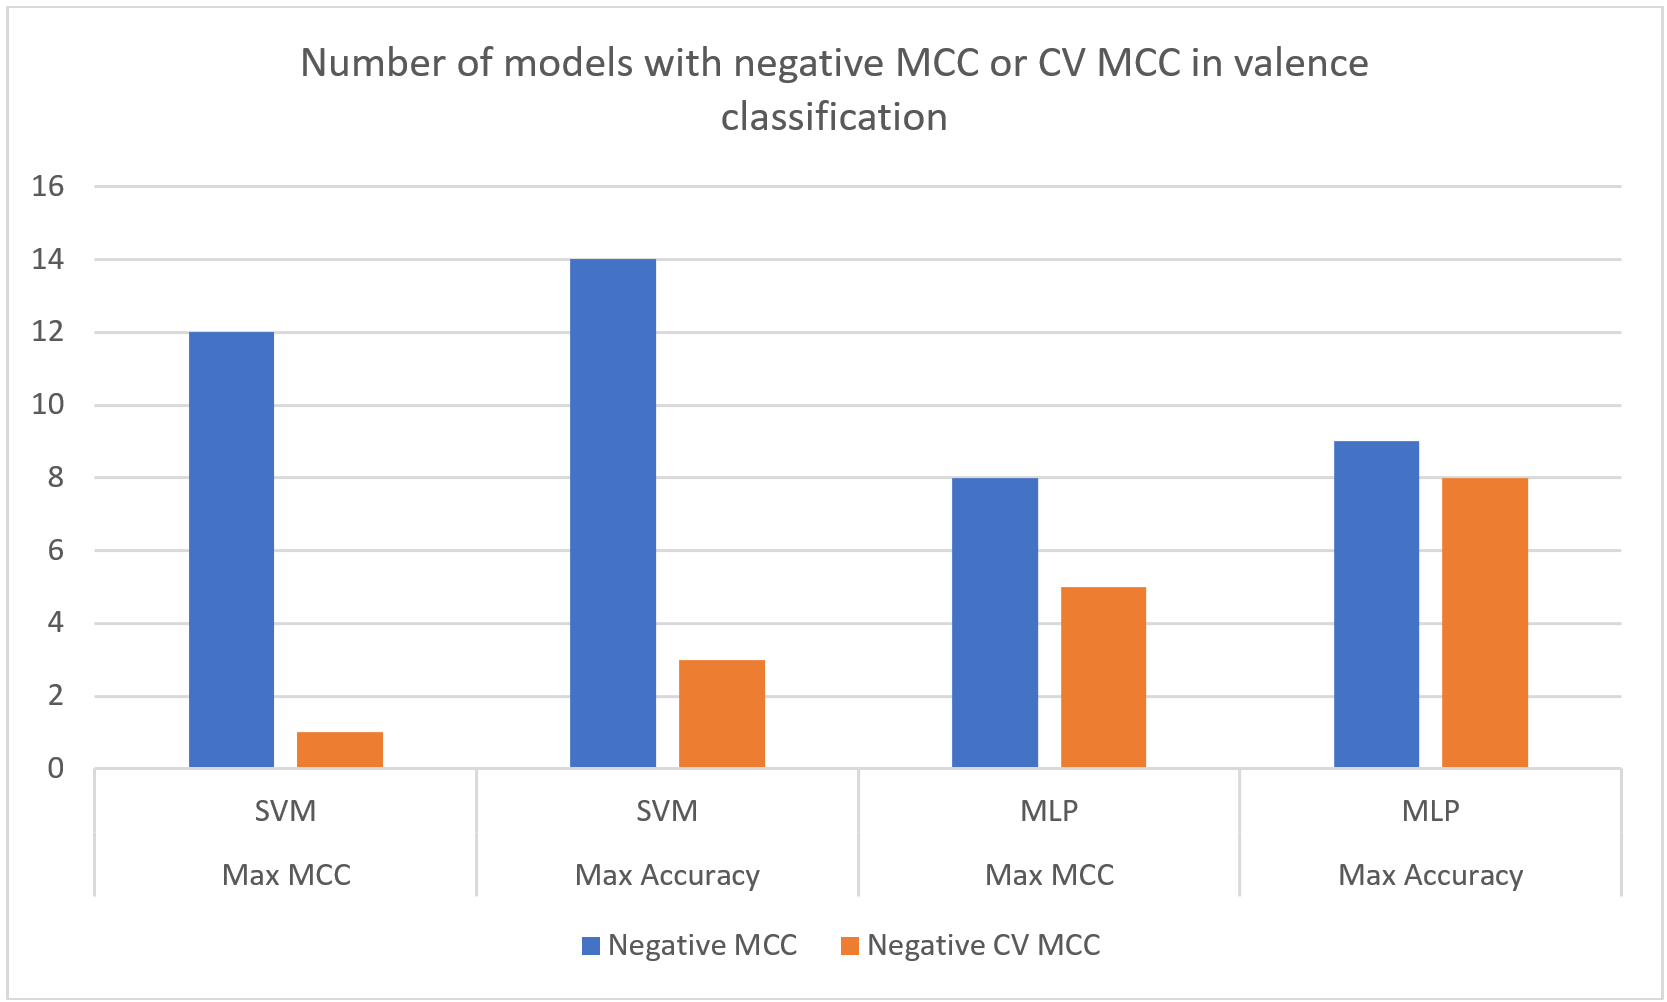
\includegraphics[width=12cm]{img/results/valence_strategy_comparison.png}
\centering
\caption{Comparison between optimization strategies of negative MCC and CV MCC scores counts for arousal classification.} \label{fig:valence_strategy_comparison}
\end{figure}

The current research is more focused on obtaining more interpretable and valid results from the classification of emotional valence and arousal rather than blindly maximizing the accuracy scores of the classifiers. The “Max Accuracy” strategy is less benevolent towards a general approach and generates more over-fitted or under-fitted models than “Max MCC” strategy, therefore results obtained using the latter strategy are considered the final ones and compared with the related work in the following section.



\chapter{Results}
\label{chap:results}
In this chapter the results of the classification using “Max MCC” optimization strategy are presented. Some premises are necessary before proceeding with the interpretation of the data:

\begin{figure}[h!]
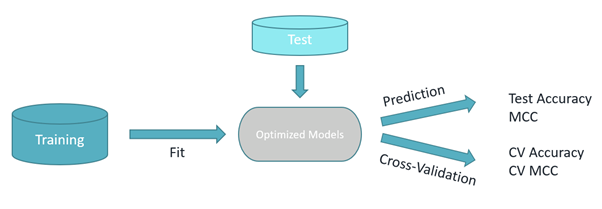
\includegraphics[width=12cm]{img/methods/data_split_strategy.png}
\centering
\caption{Approach used to compute Test Accuracy, MCC, CV Accuracy and CV MCC with separate splits of data.} \label{fig_data_split_strategy}
\end{figure}

\begin{enumerate}
\item 	The average scores at the bottom of each table are between models with the same architecture, but different hyper-parameters. Furthermore, having an accuracy lower than the chance level but with a positive \ac{MCC} has been preferred compared to have the highest possible accuracy with a zero or negative \ac{MCC}.
\item 	CV Accuracy, CV Acc Std, \ac{CV MCC} and CV MCC Std stand for Cross-Validated Accuracy and MCC and their respective standard deviation.
\item 	Test accuracy and \ac{MCC} are computed using an unseen test split of the data. CV Accuracy and \ac{CV MCC} have been computed on the training split of the data; thus, their purpose is to provide a measure of consistency of the test scores (see Fig \ref{fig_data_split_strategy}).
\item 	The confidence interval has been calculated on the test split, Z=1.96. Chance level represents the default guessing of the majority class.
\end{enumerate}

First, the classification performances of \ac{SVM} and \ac{MLP} are compared for both arousal and valence classification. Then, the performances between “Max MCC” and “Max Accuracy” strategies are compared, and the criteria to choose “Max MCC” as preferred one are explained. Finally, the results are compared with related work.

\section{Support Vector Machines vs Multi-Layer Perceptron}
\label{sec:svm_mlp}
The results of the subject-dependent arousal classification experiment are reported in Table \ref{tbl:arousal_results}, while the results for valence classification are reported in Table 2. In arousal classification, the highest and consistent test accuracy score is 81\% with \ac{MCC} score of 0.61 using \ac{SVM} and 80\% with \ac{MCC} score of 0.61 using \ac{MLP}. The 5 highest consistent accuracy scores for each classifier have been highlighted in light blue for comparison. \ac{SVM} obtained higher average test accuracy score of 63\% (0.09) and average \ac{MCC} score of 0.18 (0.20), with only 5 models scoring \ac{MCC} \(\leq 0 \) and no model scoring \ac{CV MCC} \(\leq 0\), while for \ac{MLP}  7 models scored \ac{MCC} \(\leq 0\) and 6 models scored scoring \ac{CV MCC} \(\leq 0\).

\begin{table}[h!]
  \caption{Arousal classification results using MCC as scoring parameter for GridSearch. The 5 best performing models in terms of accuracy and MCC score are highlighted in blue, the models with MCC \(\leq 0 \) or CV MCC \(\leq 0\) are highlighted in orange and yellow, respectively.}
  \label{tbl:arousal_results}
  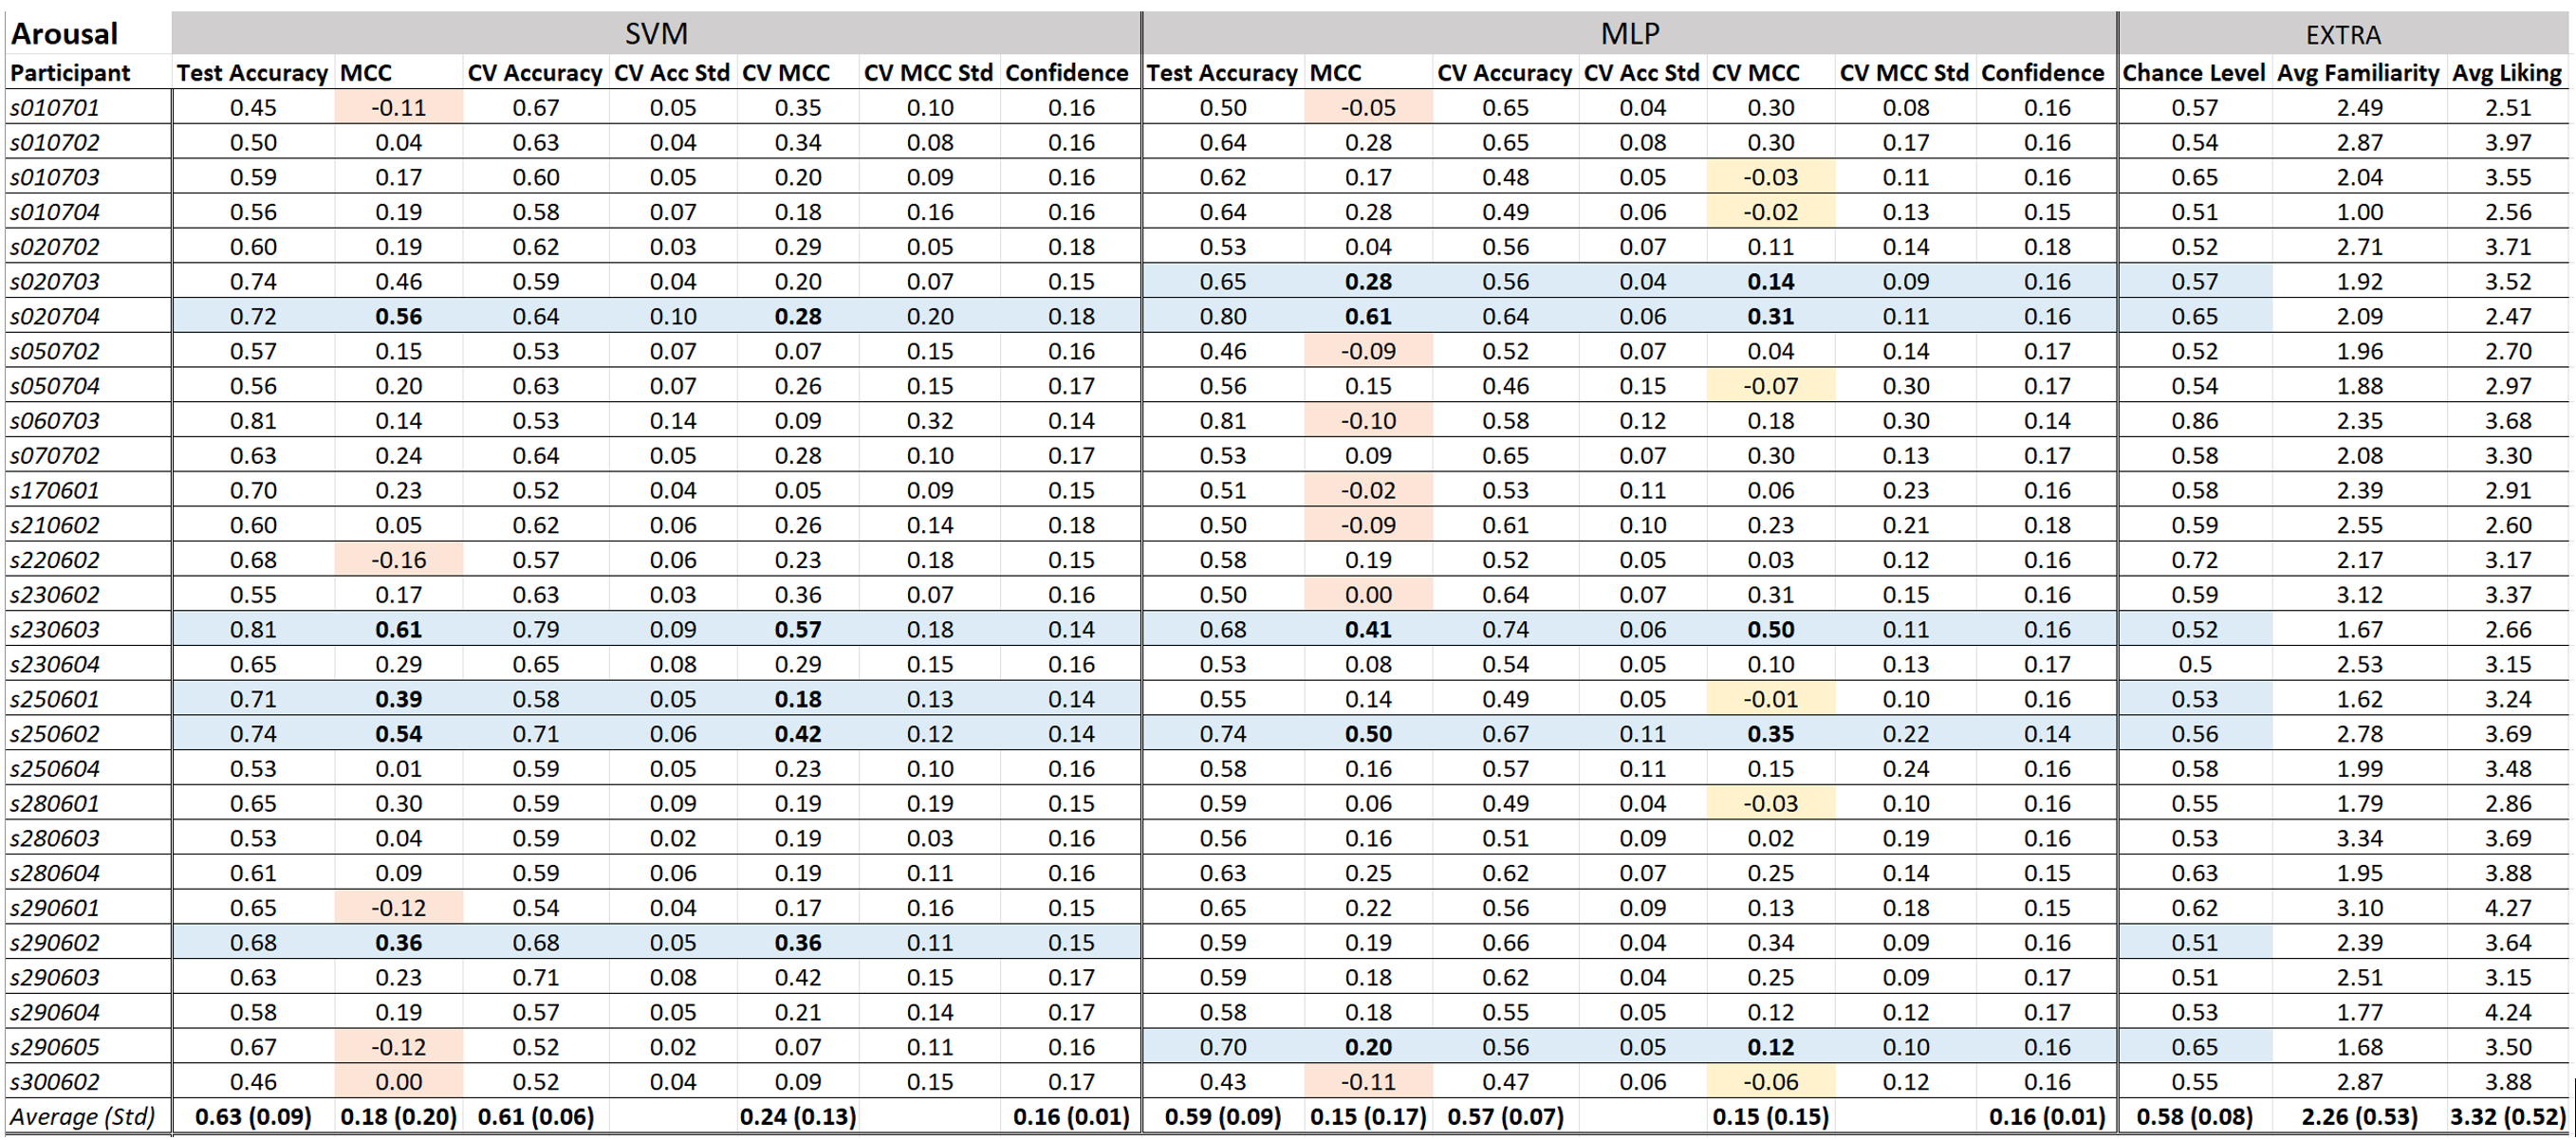
\includegraphics[width=\linewidth]{img/results/arousal_results.png}
\end{table}

For valence classification (see Table \ref{tbl:valence_results}), the highest and consistent test accuracy score is 73\% with \ac{MCC} score of 0.50 using \ac{SVM} and 74\% with \ac{MCC} score of 0.42 using \ac{MLP}. Again, the 5 highest consistent accuracy scores have been highlighted in light blue. For \ac{SVM}, average accuracy score was 65\% (0.12) and similarly for \ac{MLP} the average accuracy score was 65\% (0.11), with \ac{MLP} obtaining a higher average \ac{MCC} score of 0.13 (0.15). However, the average \ac{CV MCC} score reveals that \ac{SVM} has been more consistent than \ac{MLP}, with only 1 model scoring \ac{CV MCC} \(\leq 0 \) against 5 models for \ac{MLP}.

\begin{table}[h!]
  \caption{Valence classification results using MCC as scoring parameter for GridSearch. The 5 best performing models in terms of accuracy and MCC score are highlighted in blue, the models with MCC \(\leq 0\) or CV MCC \(\leq 0\) are highlighted in orange and yellow, respectively.}
  \label{tbl:valence_results}
  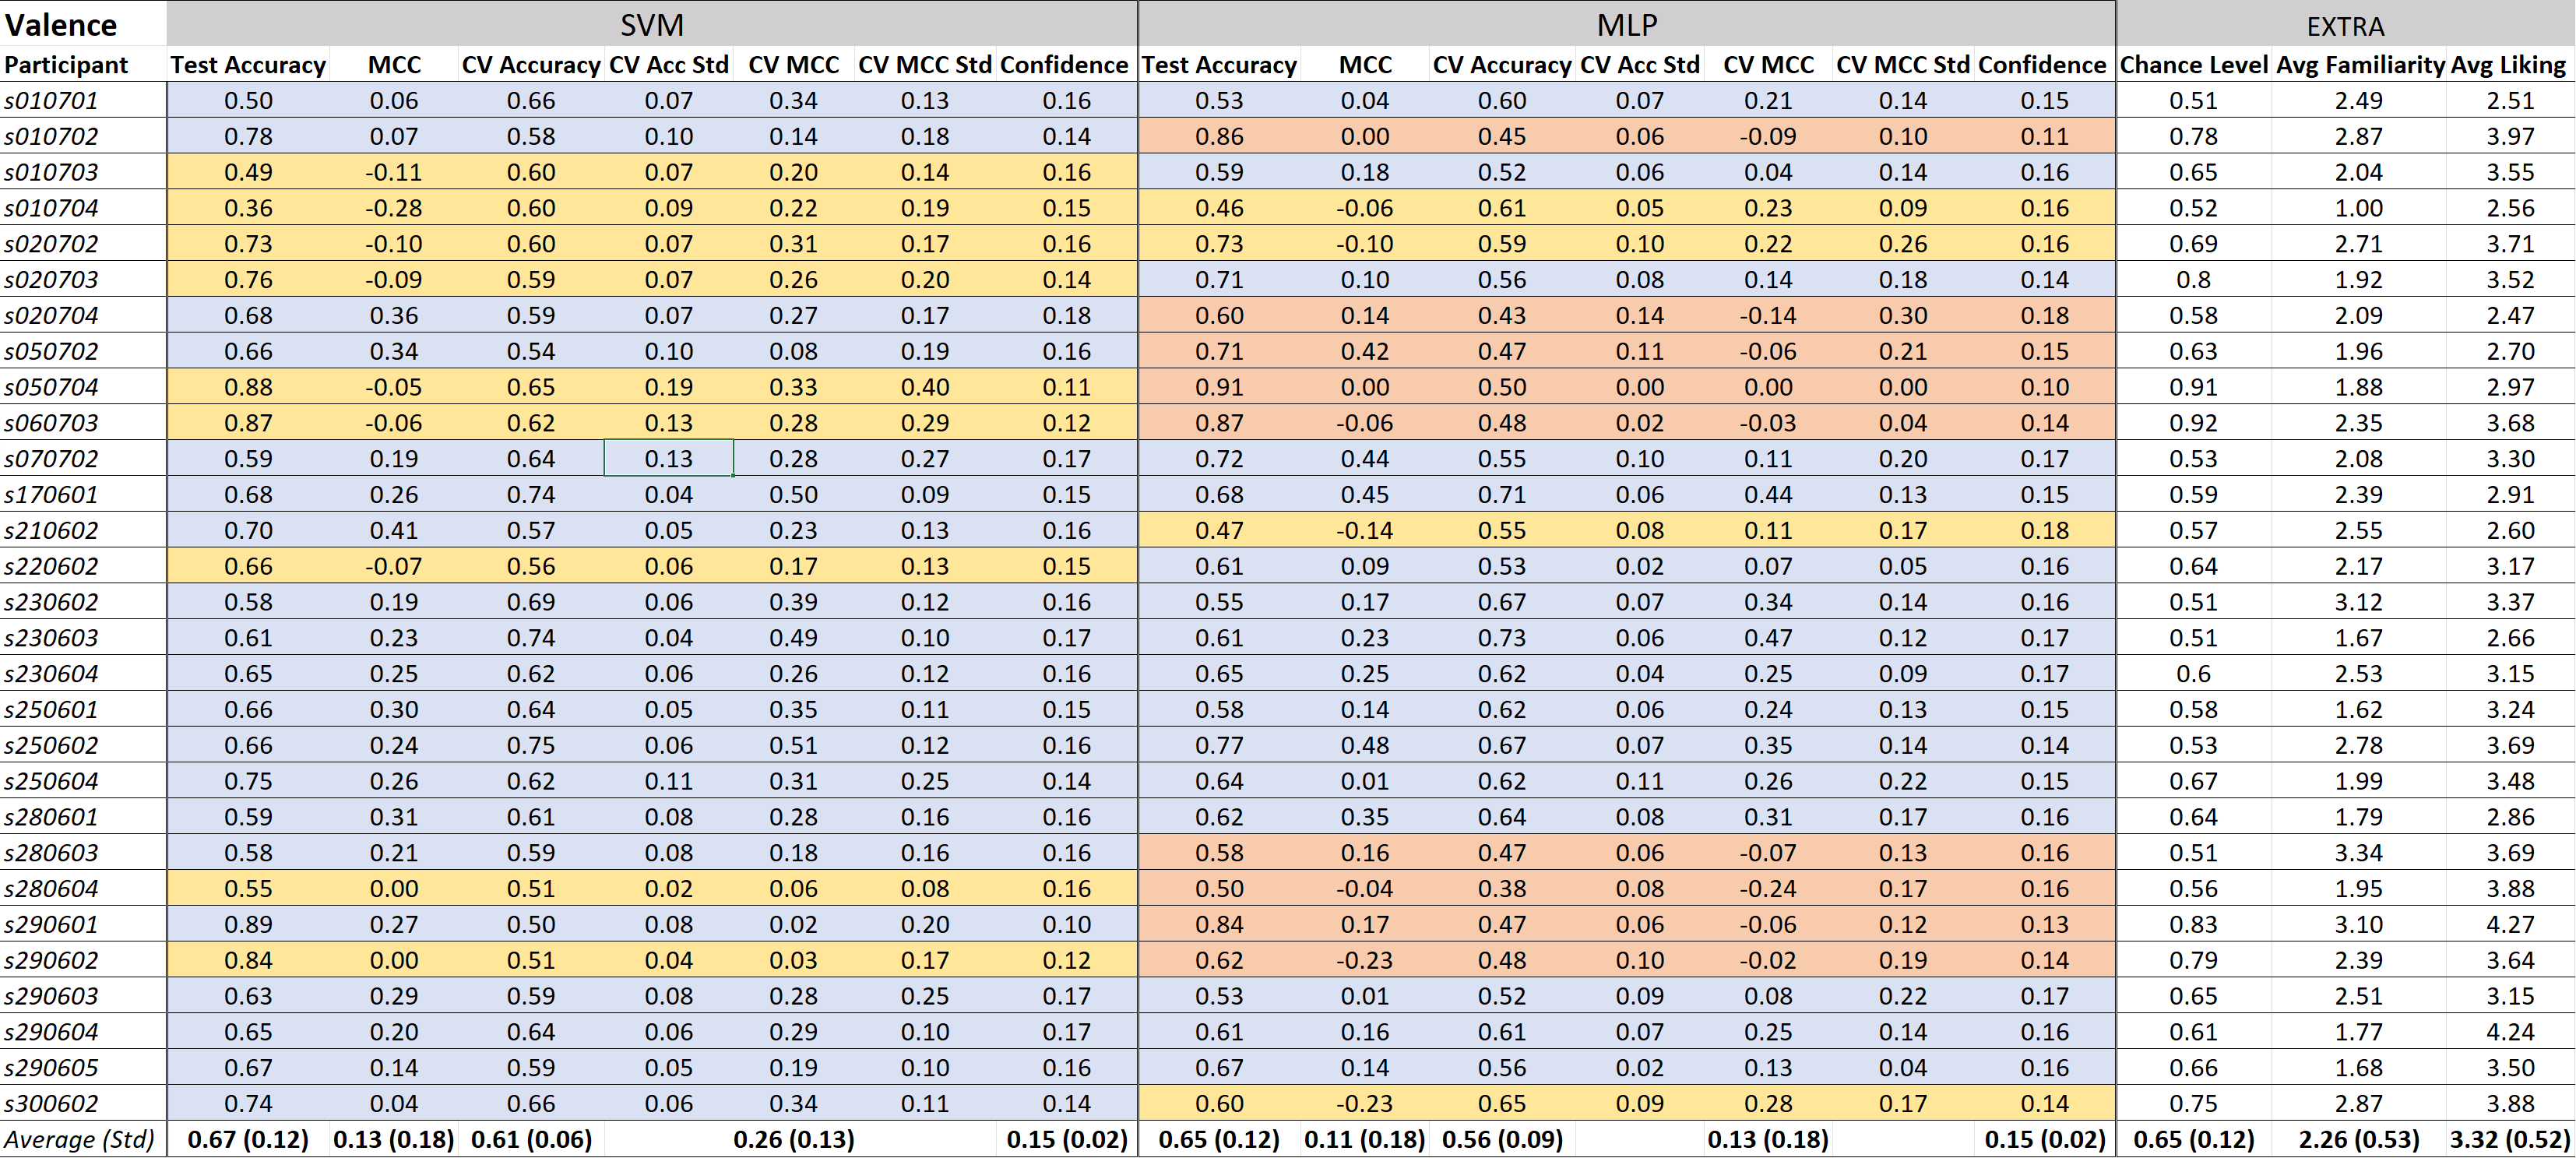
\includegraphics[width=\linewidth]{img/results/valence_results.png}
\end{table}

Overall, the classification performances between \ac{SVM} and \ac{MLP} are not significantly different, except for the Cross-Validated MCC scores that reveal a better learning consistency using \ac{SVM}. Surprisingly, arousal classification resulted in higher absolute accuracy scores and for \ac{SVM} a significantly minor number of not-learning models. This could be explained by the different distribution of labels, which for valence is more unbalanced towards the positive class (see Chapter \ref{sec:unbalanced_labelling}).

\section{Better learning or better accuracy}
\label{sec:better_learning_accuracy}
The same experiment was repeated choosing \emph{accuracy} as scoring parameter for GridSearch when tuning hyper-parameters, with “max accuracy” strategy. The purpose of this experiment was to compare the scoring strategies; however, it is important to underline that the loss function implemented in the scikit-learn library for GridSearch is chosen to optimize accuracy and only then the scoring parameter is used to select the best configuration. The results of subject-dependent arousal classifications are reported in Table 3, and they are not significantly different from the previous experiment. However, the highest consistent accuracy score using \ac{MLP} is 77\% with \ac{MCC} score of 0.53. Furthermore, it is possible to notice an increased number of negative \ac{MCC} and \ac{CV MCC} scores, and for \ac{MLP} the best performing models are not entirely consistent with the previous experiment.

\begin{table}[h!]
  \caption{Arousal classification results using Accuracy as scoring parameter for GridSearch. The 5 best performing models in terms of accuracy and MCC score are highlighted in blue, the models with MCC <= 0 and CV MCC <= 0 are highlighted in orange and yellow, respectively.}
  \label{tbl:arousal_max_acc_results}
  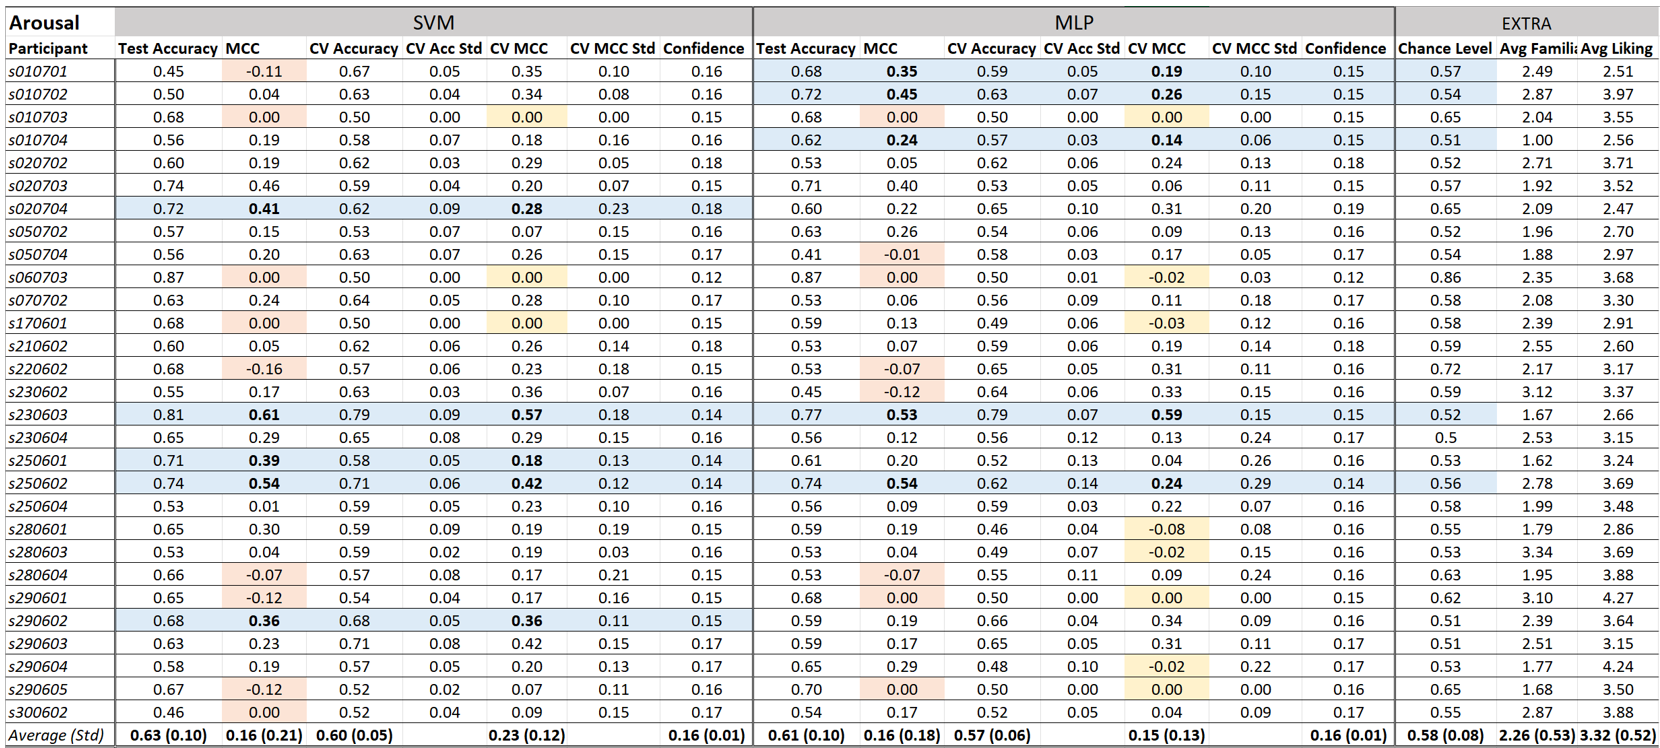
\includegraphics[width=\linewidth]{img/results/arousal_max_acc_results.png}
\end{table}

For valence classification the average test score is slightly higher for both \ac{SVM} and \ac{MLP}, but the highest accuracy score for \ac{MLP} reaches 90\% with \ac{MCC} score of 0.36. For \ac{SVM} the highest accuracy score is 80\% with \ac{MCC} score of 0.11. These highest accuracy scores are not consistent with the previous experiment and the relatively lower associated \ac{MCC} scores can be explained by the different scoring strategy.

\begin{table}[h!]
  \caption{Valence classification results using Accuracy as scoring parameter for GridSearch. The 5 best performing models in terms of accuracy and MCC score are highlighted in blue, the models with MCC <= 0 and CV MCC <= 0 are highlighted in orange and yellow, respectively.}
  \label{tbl:valence_max_acc_results}
  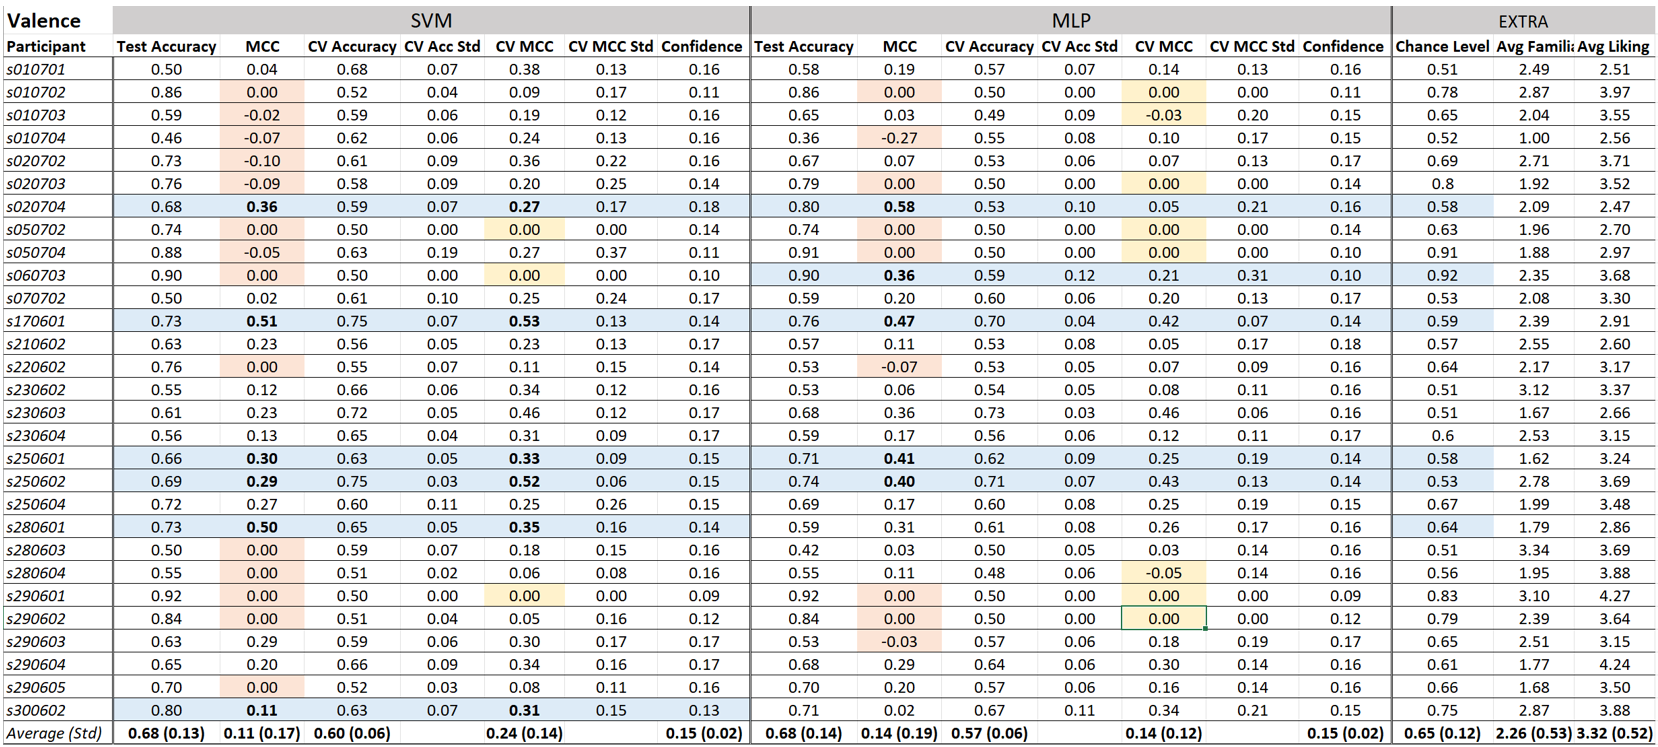
\includegraphics[width=\linewidth]{img/results/valence_max_acc_results.png}
\end{table}

Overall, it is also noticeable that an increased number of models is not learning, either because of over-fitting or under-fitting. This is particularly evident for arousal classification. This can be observed in the plots in Fig. \ref{fig:arousal_strategy_comparison} and Fig. \ref{fig:valence_strategy_comparison}, in which the number of models scoring 0 or less in \ac{MCC} and \ac{CV MCC} scores is compared between both strategies, for arousal and valence respectively.

\begin{figure}[h!]
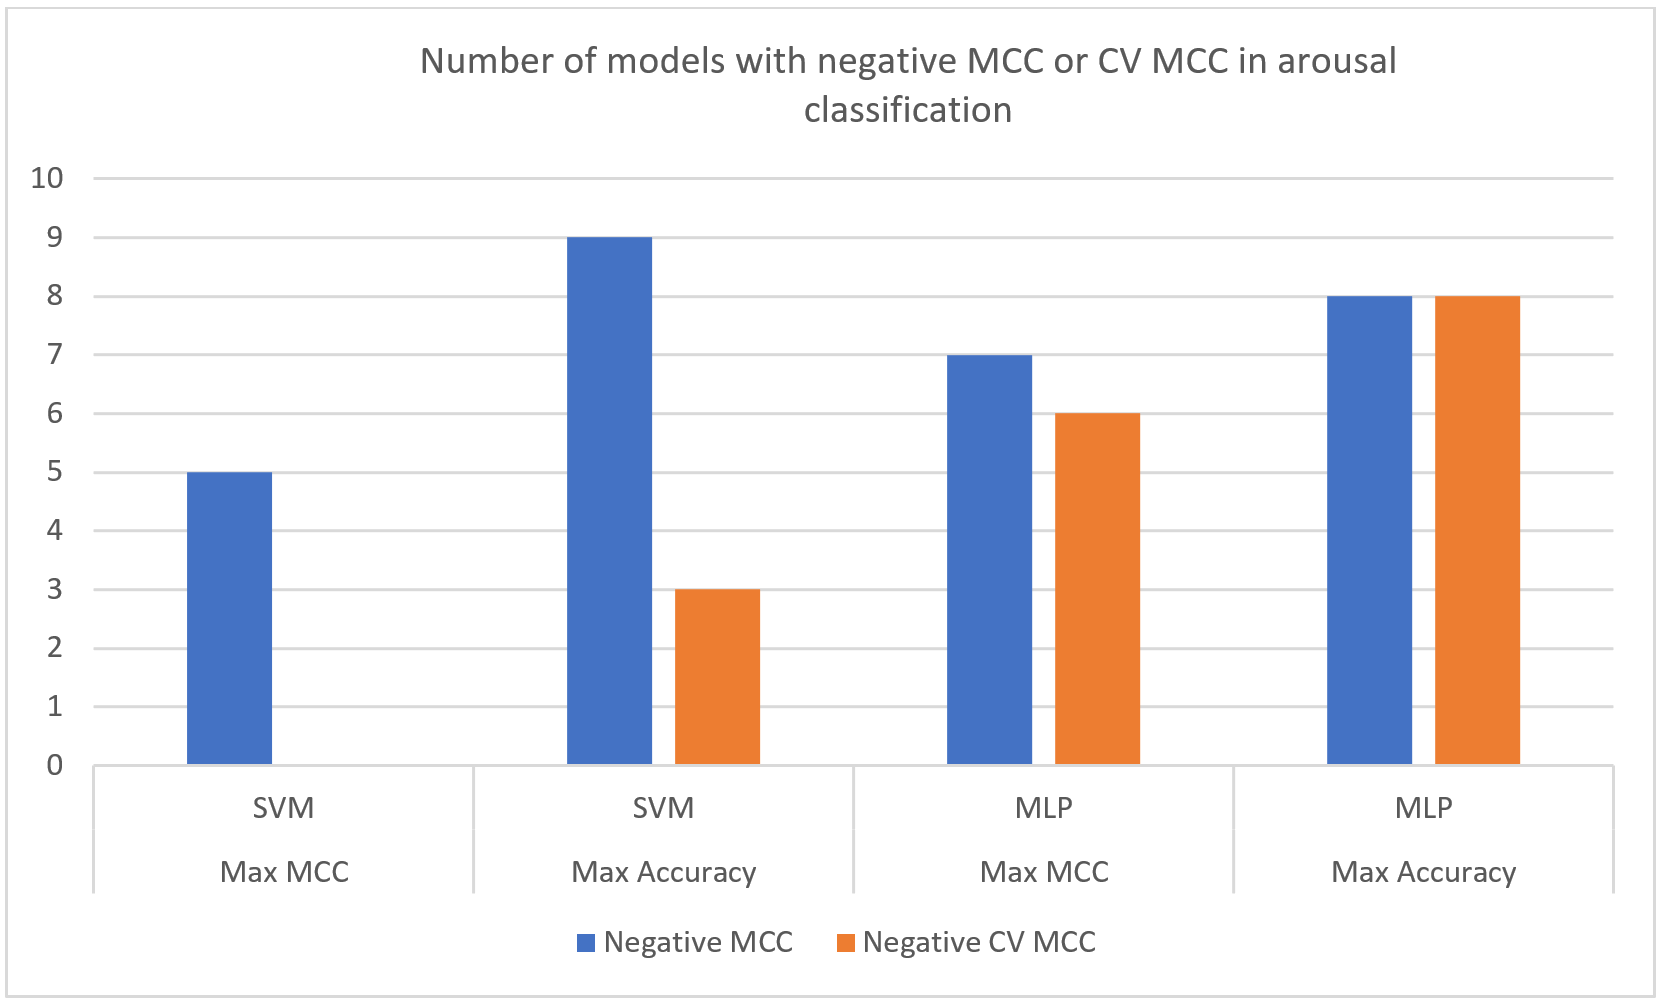
\includegraphics[width=12cm]{img/results/arousal_strategy_comparison.png}
\centering
\caption{Comparison between optimization strategies of negative MCC and CV MCC scores counts for arousal classification.} \label{fig:arousal_strategy_comparison}
\end{figure}

For arousal classification the difference between Max MCC strategy is evident and significant for \ac{SVM} classifiers, and there is increasing trend between Max MCC strategy and Max Accuracy Strategy. In valence classification the difference is less remarkable, but the same increasing trend between the two strategies is present.

\begin{figure}[h!]
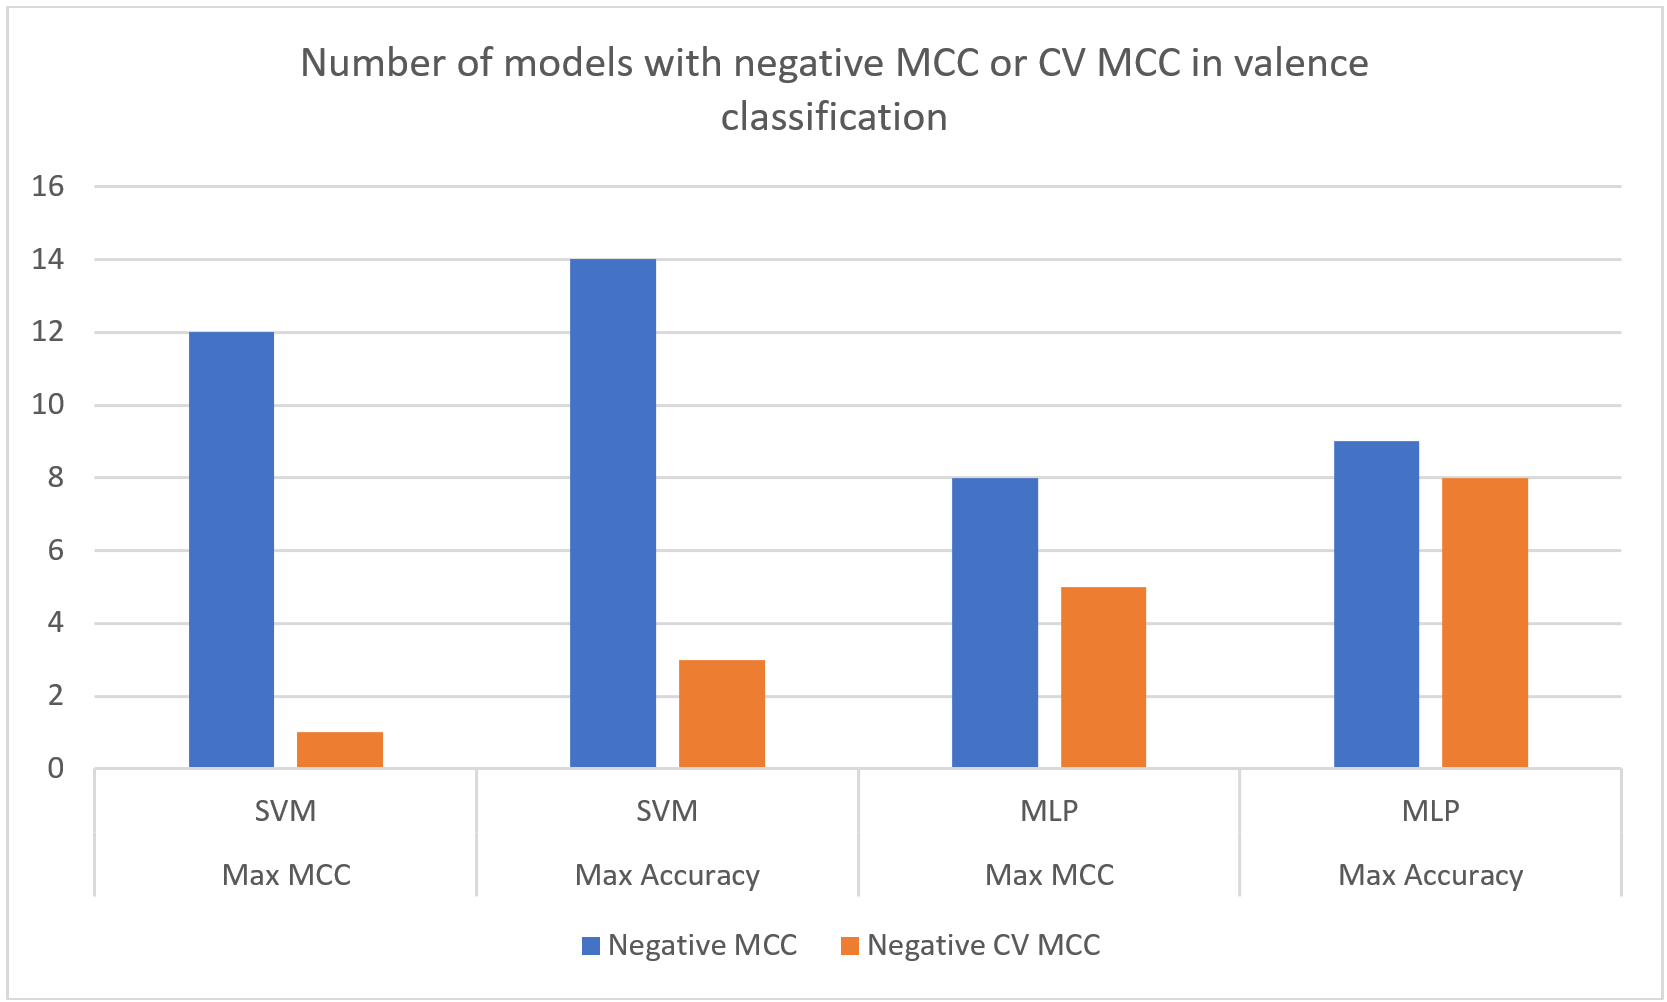
\includegraphics[width=12cm]{img/results/valence_strategy_comparison.png}
\centering
\caption{Comparison between optimization strategies of negative MCC and CV MCC scores counts for arousal classification.} \label{fig:valence_strategy_comparison}
\end{figure}

The current research is more focused on obtaining more interpretable and valid results from the classification of emotional valence and arousal rather than blindly maximizing the accuracy scores of the classifiers. The “Max Accuracy” strategy is less benevolent towards a general approach and generates more over-fitted or under-fitted models than “Max MCC” strategy, therefore results obtained using the latter strategy are considered the final ones and compared with the related work in the following section.

\section{Comparison with related work}
\label{sec:comparison}
Comparing the result of the current research with related work is non-trivial because of the methodological differences in data collection, processing, and evaluation. These differences have been considered to sort the comparisons from most comparable to least comparable. 
\\
The first and most comparable study [31] used self-reported continuous annotation as main labelling method for classification, the data were collected from 9 subjects with a wearable EEG headset equipped with 8 dry electrodes and processed using the automated PREP pipeline in MATLAB. The accuracy scores of SVM classifiers using EEG and LOBO cross-validation are only reported through plots, valence classification scored average accuracy of ~68\% and a standard deviation ~0.10, and arousal classification scored average accuracy ~64\% and a standard deviation ~0.10. The current study reports average test accuracy of 65\% (0.12) and average LOBO cross-validated accuracy on the training set of 61\% (0.07) for valence classification using SVM classifiers. Arousal classification scored an average test accuracy of 63\% (0.09) and average LOBO cross-validated accuracy of 61\% (0.06). They provided a table reporting the MCC scores for each classification modality, the average CV MCC reported for valence is 0.247 (0.17) and the average CV MCC for arousal is 0.177 (0.04). The current study reports average test MCC score of 0.10 (0.15) and average CV MCC score of 0.26 (0.15) for valence, while for arousal the average test MCC score is 0.18 (0.20) and average CV MCC score is 0.24 (0.13). Finally, the individual highest CV MCC score reported is 0.596 (0.3) for valence and 0.23 (0.22) for arousal, while in the current study the highest CV MCC score reported is 0.53 (0.13) for valence and 0.57 (0.18) for arousal, using SVM. These results are aligned with the current study and provide individual insights for each subject that can be easily compared.
\\
The second comparable study [26] is the one that inspired the self-reporting of emotions using continuous annotation. The focus of this study, however, was to compare traditional discrete annotations to continuous annotation and to evaluate two approaches for features extraction. For comparison purposes, the scores reported using PSD features will be considered instead of the scores obtained with FD features. The accuracy scores, and relative standard deviations are mostly reported in plots and partially during the discussion, so an estimate is provided. Using SVM, valence classification score is ~81.2\% (0.08) average CV accuracy and arousal classification score is ~75\% (0.08) average CV accuracy. With MLP, valence classification score is ~80.2\% (0.1) average CV accuracy and arousal classification score is ~75\% (0.1) average CV accuracy. These scores are significantly higher than chance level and clearly outperform the results obtained in the current study, that are not on average significantly higher than chance level. No further insights are provided on individual performances, so they can be considered not relevant. 
\\
The third study [25] aimed at artificially simulating a wearable device by selecting, 2, 4 and then 8 frontal electrodes from the subjects of the DEAP dataset, collected with and EEG system with 32 wet electrodes and discrete self-reported labels. Only the results for the 2 electrodes configuration using SVM for subject-dependent classification are reported and no specific description of the preprocessing pipeline is provided. The average CV accuracy scored for valence classification is ~68.4\% (0.02). The authors also provide better scoring using GBDT classifier for subject-dependent and subject-independent classification and a balancing strategy for the labels is explained, but no specific distribution of positive and negative class is provided, nor individual insights for subject-dependent classification.
\\
The fourth and last comparable study [23] collected self-reported continuous annotations from 26 subjects using a standard EEG system with 32 wet electrodes. The data were preprocessed with visual inspection on EEG lab and then features were extracted from 12 pairs of symmetrical electrodes. The authors provide 3 classifications schemes, but only the “one-against-one scheme is comparable in terms of binary classification of valence and arousal and therefore reported. The reported CV accuracy score for valence classification is 94.86\% (0.176) and for arousal classification is 94.43\% (0.212). The authors did not report the distribution of the classes.


\chapter{Discussion}
\label{chap:discussion}
In this chapter, the research results are discussed and contextualized with the research questions (see Chapter \ref{chap:introduction}) and the idea that inspired this work: evaluating the feasibility of performing real-time Emotion-Recognition with a wearable device for a future affective \ac{BCI} system. 

\section{Challenges towards real-time Emotion-Recognition}
\label{sec:challenges}
When imagining users adopting a technology in their life, many functional and design aspects are rightfully expected. For example, the design of the device needs to be sleek and intuitive, and the flow of the application must be seamlessly integrated and well performing. This is clearly not the case for current Brain-Computer Interfaces, that are still in their infancy and far from mass adoption, especially for non-clinical applications. Lin, Jung and Onton \cite{lin_toward_2015} reviewed a collection of methods that could greatly improve the quality of the user experience and finally open the way for affective \ac{BCI} to reach the consumer market. The core challenge of affective \ac{BCI}  is to create a plug-and-play \ac{BCI}  system with limited electrodes that can consistently perform accurate Emotion-Recognition regardless from the person that is using it. The other challenges consequently follow:
\begin{itemize}
\item 	\textbf{Reduction and selection of electrodes:} the number of electrodes must be relatively small, between 2 and 8, and strategically placed over the cortical areas delegated to the processing of emotions. They also should be soft dry electrodes and the system should be able to automatically recognize bad channels and excluding them from the processing.
\item 	\textbf{Automatic artifacts cleaning}: artefacts are one of the most impacting problems, and currently the most popular approaches for offline artifact cleaning are \ac{ICA}, that is not applicable to small sets of electrodes and too computationally expensive for online cleaning, and visual inspection. Alternative approaches might be achieved using regression to train algorithms in recognizing specific types of artifacts or features of the signal that indicate whether the quality is good or not and adjust it accordingly. Cleaning artifacts is also vital to the efficient use of as much data as possible. In the current study the artifacts removal strategy led to the exclusion of 10 participants and the removal of up to 25\% of the data of the remaining participants, a considerable cost considering the time and efforts needed to collect the data with an experimental protocol.
\item 	\textbf{Features selection and reduction}: selecting the most suitable features allows to reduce the computational cost by removing redundant and less meaningful features, and this is particularly correlated to the selection of electrodes as well. Lin et al. \cite{lin_toward_2015} through their extensive research over the years discovered that differential asymmetries are the most consistent type of features among subjects and sessions, reliable also for subject-independent classification. In more recent studies, Thammasan et al. \cite{thammasan_continuous_2016}, Keelawat et al \cite{keelawat_comparative_2021} and Avramidis et al. \cite{avramidis_multiscale_2021} , extracted \ac{EEG} features using fractal dimension algorithms instead of \ac{PSD}, obtaining significantly better performances in both subject-dependent and subject-independent classification. Another possibility is to use more complex models like \ac{CNN} \cite{keelawat_comparative_2021} to automatically extract features from the \ac{EEG} signal, sacrificing the ease of interpretability of the model and the direct connection with the theoretical neuroscience.
\item 	\textbf{Users training and calibration}: a very time consuming and frustrating process is the calibration of \ac{BCI} systems for new users, especially if they have no experience of brain-controlled inputs. A system that can only classify emotions with a subject-dependent strategy is bound to train the users in reporting their emotions and then train a classifier with the collected data, all under the assumption that the resulting dataset is not too unbalanced. This of course is not feasible, and ultimately subject-independent classification should be the aim for real-time systems. However, this might not suffice, and even subject-independent classifiers might have to be tuned with short calibration sessions to adjust for each specific case, for example by selecting more susceptible features for a certain user that matches similar brain “signatures” from a group of users that the model has already been trained on. Zero-training strategies \cite{krauledat_towards_2008,jeong_hybrid_2021} have been object of study over the last decade and using spatial filters and transfer learning makes it possible to train a sub-optimal decoder and then use unsupervised learning to transform it into a user specific decoder. Of course, these solutions are still very experimental and use case specific, and further investigation is required.
\end{itemize}

The rest of the chapter will contextualize these challenges in the current study. Using a wearable EEG is a solution to the first problem, but also a constraint around which every other problem had to be worked around.

\section{Self-reported emotional labels}
\label{sec:self_reported_labels}
Reporting emotions is a non-trivial task and could be subjectively difficult. From the feedback forms collected after the experiment, 7 subjects reported to have found difficulties in choosing the quadrant of the valence-arousal space, 8 subjects reported difficulties in assessing the emotional intensity (in both dimensions) and 9 subjects reported difficulties in assessing the specific emotions. In addition, participants reported an average fatigue score of 2.47 ± 0.97 after the first half of the experiment and a fatigue score of 3.27 ± 0.86, on a scale from 1 to 5. Some emotions were reported to be missing from the simplified valence-arousal space, for example "annoyance". Another missing emotion was “bittersweet”, that is commonly experienced in music listening yet difficult to report because of its composition of not-adjacent emotions (sadness, happiness) on the valence-arousal space. Continuous annotation of emotions has several advantages over discrete annotation, allowing a more granular reporting that consider emotional “oscillations” over the duration of a stimulus and more distributed labels across all classes that can favor the classification task.  It is a powerful tool for researchers to build affective datasets but heading towards a real product it will eventually be an obstacle as it requires an extra layer of training before the calibration. Discrete annotations are a simpler task that has virtually no impact on the recording phase and can be more easily integrated in a calibration tool, but seemingly yielding poorer performances compared with the continuous approach \cite{thammasan_continuous_2016}. An example to compromise the benefits of both approaches could be a subject-independent classifier trained using an offline dataset collected with continuous labelling, then discrete annotations collected by an online system would be used to integrate subject-specific differences during a calibration phase.

\section{Familiarity, liking and PANAS}
\label{sec:familiarity_liking_panas}
During the experiment, participants were asked to rate every song they listened to in terms of how much they liked the song referred to as “liking” and how much the song was familiar to them referred to as “familiarity, both on a scale from 1 to 5 where “3” represents neutrality. These scores could be used in a music recommending system to enhance the quality and relevancy of recommendations, however for the current research they were only used to assess the impact of the selected stimuli. The average “liking” score across all trials and all participants 3.32 ± 0.52, indicating that the selection has been in general positively perceived. Average “familiarity” score was 2.26 ± 0.53, quite below neutrality despite most of the songs being from internationally known artists. Having general low familiarity is positive for classification as emotional biases caused by memories can occur. Looking at Tables \ref{tbl:arousal_results} and Table \ref{tbl:valence_results}  in the previous chapter it is also possible to observe that some of the participants with highest average “familiarity” are also among the worst classification scores, but the analysis was out of the scope of this research. Further investigation is needed regarding the correlations of “liking” and “familiarity” with the emotional dimensions of valence and arousal. Before each session, participants were also asked to fill a PANAS questionnaire. 

\begin{figure}[h!]
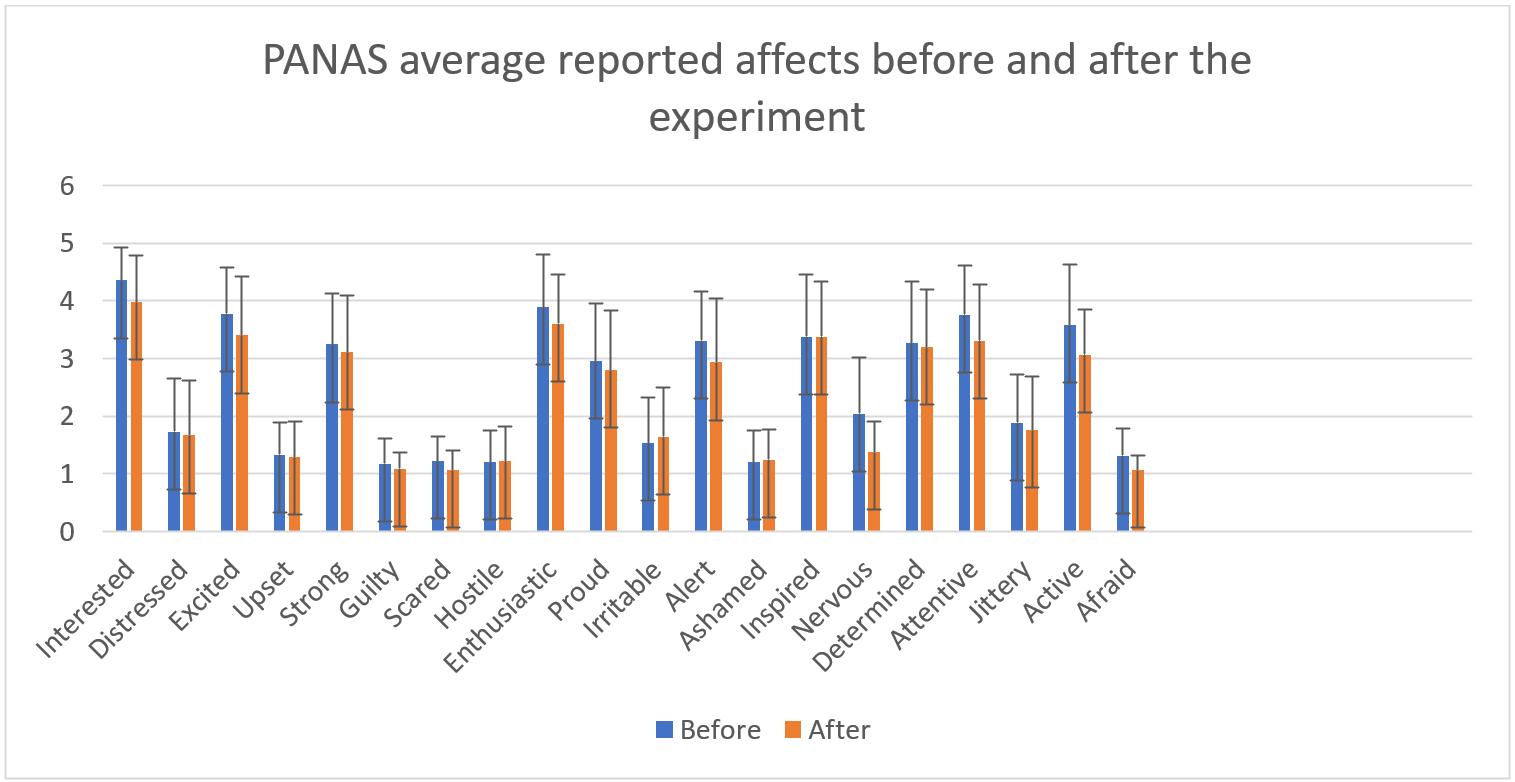
\includegraphics[width=12cm]{img/discussion/panas.png}
\centering
\caption{Average reported affects before and after the experimental session.} \label{fig:panas}
\end{figure}
Comparing the assessed affects before and after the experiment (Fig. \ref{fig:panas}), it is possible to observe that general interest, enthusiasm, and excitement of the participants decreased, which was expected considering that for the majority of the participants it was the first time participating in an EEG experiment. Attentiveness and activeness also significantly decreased, suggesting that the task proposed, and the length of the session were to some degree causing fatigue. Follow-up experiments can account for these effects by shortening the length of musical excerpts, reducing the number of conditions, or distributing the data collection from each participant over multiple sessions.

\section{Features selection and performances evaluation}
\label{sec:features_performances}
The proposed principal features based on previous findings on differential and rational asymmetries were the neuromarkers: \ac{AWI}, \ac{FMTI} and \ac{SASI}. The frequency-band specific features of the \ac{EEG} signal were extracted using the \ac{SPT} proprietary library from myBrainTechnologies. Intermediary experiments using forward \ac{SFS} revealed a general trend in selecting the neuromarkers as most significant features, with some exceptions. \ac{PCA} was then used instead of \ac{SFS} as better performing subject-dependent features selection method to reduce the dimensionality of the features vector in lower computational time. It was not possible to directly compare the impact of using neuromarkers instead of frequency-band specific features, but the results were very promising for a subset of participants. The evaluation of model performances using \ac{MCC} score led to better understanding and correcting models who were over-fitting toward the majority classes because of uneven distributions of labels. It made possible to easily identify under-fitting models too, however no solution was found to prevent it. Overall, \ac{MCC} score seems to be a more reliable score to describe the learning capabilities of the models, and it is better for comparison with the most recent related studies that make use of it, instead of classification accuracy only.

\section{From subject-dependent to subject-independent classification}
\label{sec:sd_to_si}
Clearly, subject-dependent classifiers are not an optimal solution for a real-time system and pose a threat to the usability by requiring full training sessions for new users. Besides, training a separated model for each user is not a long-term scalable solution. However, due to the subjective differences, subject-dependent remains the current preferred choice for Emotion-Recognition. Subject-independent strategy is only applicable to set of features that can represent the same emotional patterns for everyone, for example differential asymmetry was reported to be very promising \cite{lin_toward_2015}, but also assumes that all the datasets used for training are as clean as possible to prevent the contamination of artefacts. In the current study it was not possible to obtain better than default-guessing during intermediate experiments on subject-independent classification. Some conditions are likely to hinder classification:

\begin{itemize}
\item 	Artifacts: Data might be too affected by artifacts, hindering any classification.
\item 	Features: Selected features might not be suitable for all subjects, or they might be suitable only for groups of subjects with similar “brain signature”.
\item 	Labels: Distribution of the classes can be highly uneven, and self-reported labels can be unreliable.
\item 	Electrodes: Two electrodes might not contain sufficient significant data; they can be misplaced or bad conducting.
\end{itemize}
The enormous performance difference among subjects in subject-dependent classifications suggests that improvements in the first three conditions are not only possible, but also necessary towards the creation of wearable affective \ac{BCI}s. If the low number of electrodes were the main impediment to classification, it would not have been possible for some participants to score more than 80\% classification accuracy. After reducing the variability created by these conditions and once subject-dependent classification will yield consistent performances among subjects, it will be possible to further develop a hybrid paradigm where a subject-independent classifier serves as sub-optimal basis for fast calibration of subject-dependent classifiers. Finally, if these goals are met, full subject-independent classification will be the next step towards affective \ac{BCI}s.

\section{Reflections on future research}
\label{sec:future_research}
The analytical study of emotions is heavily impacted by subjective differences, and the current state of art technology and signal processing techniques still struggle to provide the desired performances to build seamless affective \ac{BCI} systems. Many critical factors starting from the data collection phase to the classification task can hinder the expected outcome. Considering the interest in a follow-up study, the factors that mainly affected the current study are addressed in the paragraphs below. 
\\
\\
\emph{Selection of the stimuli.} The selection of the stimuli is critical for the success for affective experiments, as there is nothing worse than selecting ineffective stimuli. Music is usually a favorable stimulus, since only a few subjects do not react at all to it. Even so, subjective preferences can highly impact the perception of the same song in a population of participants. This study conveniently “recycled” a selection of songs previously used in other experiments and proposed the same playlist to all participants for the sake of inter-subject comparison. This choice led the participants to a constrained experience, that for some resulted in listening to music genres they usually would not listen to. In addition, the annotation experience suffered of great variability, leading some subjects to never report some one or more valence-arousal classes. There are alternative solutions for the stimuli selection, as some related studies experimented \cite{thammasan_continuous_2016}. For example, the researcher can ask the subjects to pick music from a selection that covers the emotional spectrum during a pre-listening phase. A better compromise could be a hybrid selection: part of the stimuli selected by the researchers and the other part selected by the participants. Adapting the selection to account for the subjective preferences is very time consuming in the design of an experiment, but it is also what real users of an affective recommending system would expect.
\\
\\
\emph{Self-assessment of emotions.} As several participants reported, it was not always simple to assess in real-time perceived emotions, with the consequence of unreliable annotations. On one hand, knowing exactly what feelings are being experienced requires considerable self-perception. On the other hand, models for assessing emotions have limitations. As mentioned earlier (see Chapter \ref{sec:self_reported_labels} ), the \ac{VA} space used in the experiment was simplified to make it more understandable, sacrificing the representation of some emotional states. Using a more complete representation does not automatically improve the participants ability to report emotions, on the contrary it is likely to introduce more confusion. Other studies \cite{lin_eeg-based_2010} adopted an even more simplified version that only associates one emotion to each quadrant of the \ac{VA} space, that maybe partially explains the significantly better performances in classification. Continuous emotion annotations require more effort but are very valuable to capture emotion oscillations and provide classifiers with more realistic emotional distribution. Once the models for the classification of emotion will have reached maturity, continuous annotations will be discarded in favor of discrete reports, that better suit a real product. The solutions for Emotion-Recognition cannot possibly start from a complex representation of emotional states, thus building up from more simplified models might be a better strategy now to support the ongoing development of the field and then later scale up the complexity with more sophisticated tools.
\\
\\
\emph{Experimental sessions.} Two main observations were made based on the feedback received and the analysis of data. First one, a single session of 75-90 minutes (30-35 of \ac{EEG} recording) can be fatiguing for most people. Decreased attention and discomfort are not favorable conditions for recording brain activity and are likely to be reflected also on the emotional assessment. Second one, a single session does not ensure that classification performances are consistent for the same subject over time. External factors experienced prior to the session might bias the emotional perception of a subject, for example if there as a breakup with a loved one or if very good news brightened the day. In addition, the oscillatory nature of brain waves is known to generate differences in the \ac{EEG} signature of the same person over time. Multiple shorter session can prevent fatigue by reducing the overall mental load, and at the same time mitigate the effect of variations over time in the emotional assessment and in the \ac{EEG}.  
\\
\\
\emph{Automated lightweight preprocessing.} The requirements for a preprocessing pipeline in an online system are not easy to meet. Computational time needs to be in the order of seconds or even better milliseconds; at the same time the quality of data must be ensured to prevent poor classification performances. Ocular artifacts are the greatest threat in the analysis of emotions because of the topological position near the frontal lobe, where emotions are processed. Using \ac{EOG} to subtract eye movements from the EEG signal is effective for offline studies but is clearly not suitable for a product. Methods like \ac{ICA} and \ac{PCA} are very effective for \ac{EEG} recordings using standard equipment with many electrodes, but nevertheless computationally expensive. For a final product using wearable devices with limited capabilities, inferring the presence of artifacts by classifying \ac{EEG} based on the signal qualities \cite{grosselin_quality_2019} can be achieved with low computational effort and enable surgical precision in the cleaning process. \ac{ASR} has been proven effective in artifact removal for both offline data analysis and online applications \cite{chang_evaluation_2018}, but for optimal outcome, i.e. removing artifacts and retaining the significance of the signal, it requires to be tuned using good quality \ac{EEG} samples. Investigating the best combination of approaches for lightweight processing can be a suitable research question also outside the specific scope of affective \ac{BCI}.
\\
\\
\emph{Features extraction and selection.} Selecting the right features has proved to be non-trivial and affected by subject-dependent differences. The extraction process also carries a computation cost, thus just extracting any possible feature and then apply subjective selection criteria is not feasible. The current study used \ac{PCA} to collapse the features in the minimum number of components that could account for subjective differences and retain at least 95\% of the variability of the data. The neuromarkers are a step towards the delineation of an optimal subset of features for emotional assessment but require more investigation both from neuroscience and data science perspectives to determine which combination of differential/rational measurements and EEG frequency bands are more relevant for the study of emotions. The identification of more subject-independent features, like the asymmetry indexes \cite{lin_toward_2015}, is also essential towards the development of affective \ac{BCI} systems and can be the main topic of a dedicated research. The possibility to use other physiological signals to build a multi-modal classification system has also been explored, and physiological signals were collected during this research for eventual follow up studies. A related study already assessed the increased performances that can be obtained by decision-level multi-modal fusion \cite{thammasan_multimodal_2017}, an adaptive approach to select by majority voting the optimal uni-modal sources among several physiological measurements (\ac{EEG}, \ac{ECG}, \ac{GSR}) for classification. Any system designed on other physiological data than \ac{EEG} is, however, outside the strict scope of affective \ac{BCI}.
\\
\\
\emph{Unbalanced datasets.} One of the main obstacles in training and evaluating classification models was the uneven distribution of labels. Multiple experimental sessions and subjective stimuli selection can minimize the possibility of having very unbalanced datasets, as explained in the previous paragraph. However, it would still be possible to hit the same obstacle, regardless the minimization. In the field of machine learning there are standard methods to deal with unbalanced methods. Assigning weights to the classes to penalize the prediction of the majority class is one of such methods, used in the current to improve the discriminative power of \ac{SVM} classifiers. Up-sampling of the minority class is another method that creates copies of labels and data in the training dataset to reduce the bias of the classifier. However, copying affective data does not seem optimal as it would simply repeat the same emotional pattern and will not likely cover the entire emotional spectrum of the minority class. Some studies investigated the possibility of simulating realistic \ac{EEG} data \cite{barzegaran_eegsourcesim_2019} from biologically plausible signals. Good affective \ac{EEG} data from multiple subjects could be collected for the realization of a plausible \ac{EEG}  simulator that can account for individual variability. The data generator could then be calibrated over a small sample of real \ac{EEG}  data from a real subject and be used to counterbalance the distribution of emotional classes, thus improving the classification performances.


%\chapter{Body of the thesis}
\label{chap:body}

This chapter contains a few general hints on the writing. See \cite{Leferink12,Meijerink12} for more details.

\section{Structure}
\label{sec:structure}

All chapters in between the introduction and the conclusions serve as a support for what is claimed in the conclusion. Several structures are possible, depending on the type of work. Discuss the structure of your report with your advisor before you start writing the chapters.

When a chapter consists of several sections, introduce the structure of the chapter in the initial section (which could be an unnumbered section). The particular purpose of the chapter should be introduced there as well (as is done above). In case of a comprehensive chapter, end it with a summary or conclusion.

\section{Figures and tables}
\label{sec:figures}
Use figures and/or tables only if this enhances the understanding of the reader. Refer to figures and tables using figure/table environments and labels, resulting in a combination of the chapter and figure/table number (for instance 'Figure~\ref{fig_empty}'), and indicate their purpose; otherwise the figure/table might as well be left out.  

A figure can for instance be a graph, picture, or schematic drawing. Make sure that all relevant aspects of a figure are well visible, when printed on A4 paper. Preferably use vector-oriented graphics, and minimize the use of colors, unless they can be clearly distinguished when printed to black and white.

Captions should be put below each figure, whereas they should be put \emph{above} tables. The captions should only describe what is depicted by a figure/table ('Measured attenuation as a function of frequency for cable lengths of 1~m, 5~m, and 10~m'), and not what should be concluded from it ('The longest cable has the largest attenuation for all frequencies.'). The latter should be put in the refering text. Always try to place the figure/table after the text in which it is refered, preferably at the top of bottom of a page, or in between paragraphs. Related figures can be combined in one figure environment using subfigures. 

If a figure has been copied from a different source, clearly indicate that in the caption (and ask for permission, if required). 

\begin{figure}
%Insert your figure here. Make sure that the type of figure file (eps/pdf/...) complies with your typesetter.
\caption{Empty figure}\label{fig_empty}
\end{figure}

\section{Equations}
\label{sec:equation}
Very short equations such as $I=V/R$ can be created in-line using dollar symbols; otherwise an equation environment (or related environment such as multline or align) should be used. Equations should be numbered after their last line in order to enable referencing elsewhere in the text. Equations are part of the sentences and therefore usually end with a period or comma. For example, according to Ohm's law, the current~$I$ flowing through a resistor is given by
\begin{equation}
I=\frac{V}{R}\,,
\end{equation}
where $V$ is the applied voltage, and $R$ is the resistance.

See \cite{Meijerink12} for some more guidelines or formating equations.

\section{Acronyms}
\label{sec:acronyms}
Acronyms should be introduced upon their first usage in the main body of the report. For instance once the \ac{FCC} has been introduced, it can be abbreviated to \ac{FCC}.

Introducing, using and listing acronyms is facilitated using the \texttt{Acronym} package and \texttt{$\backslash$ac} command. 

A common misconception is that the constituting words should be capitalized when the corresponding acronym is in capitals, but this is only the case when the abbreviated words form a name, such as the \ac{IEEE}. On the other hand, technical terms such as \ac{UWB} or \ac{OBFN} should not be capitalized, even though their acronyms (\ac{UWB} \ac{OBFN}) are. 

Acronyms always have to be introduced in the main body of the report, even if they have already been introduced in the summary. Therefore it is better to use the \texttt{$\backslash$ac} command only in the main body of the report, and not in the summary.

\section{Citations}
\label{sec:citations}
Use citations if the corresponding book, paper, or report supports a claim that you make in your text, or if it clarifies the context of the work (i.e. what related work have you or other people done). Only list references that are actually cited in the text; the bibliography is not just a list 'for further reading' (although that could be made separately), or a list of documents that you consulted during your work. 

If you literally copy text fragments from a different source, explicitly indicate this using quotes and italic characters. Only copy or summarize material from different sources if this contributes to the understanding of the reader; in principle your report should be readable without consulting the references.

The credibility of the claims in your text is largely influenced by the quality of your cited references: for instance papers in international peer-reviewed journals are generally more reliable than Wikipedia articles. 

Also, note that many readers will tend to judge your knowledge on the context of your work based on the references that you cite. 

Some examples are given in the References chapter~\cite{TEwebsite,Cox04,Meijerink05,Meijerink10,Meijerink06,Leferink12,Meijerink12}.

%\include{chap_...}

\chapter{Conclusions and recommendations}
\label{chap:conclusions}
The goal of the experiment setup for this research was to answer the main research question: \emph{“What are the performances of classification of music-elicited emotional valence and arousal using a wearable EEG headset?”} and the two sub-research questions that extended it. This research set out to investigate the feasibility of performing \ac{ER} using a wearable interface in the form of a classification task. Data were collected using a robust protocol in two different conditions. They were then processed using a lightweight automated preprocessing pipeline and two types of features were extracted: neuromarkers and frequency-band specific spectral features calculated in the Theta, Alpha and Beta bands of the \ac{EEG} signal. Features dimensionality was reduced using \ac{PCA} and the classification task was performed with subject-dependent strategy. The problem was simplified into two separate binary classifications for valence and arousal, and two algorithms were tested: \ac{SVM} and \ac{MLP}. The hyper-parameters were tuned using GridSearch to select the configuration that yielded the highest \ac{MCC} score. All models were then trained and tested using 5-fold \ac{LOBO} cross-validation that produced two cross-validated scores: \ac{CV} accuracy and \ac{CV MCC}. Then, models were further tested on a completely unseen split of data that produced two more scores: test accuracy and \ac{MCC}. Each question is answered separately in the following section and then some recommendations for future work are proposed in the last section.
\section{Conclusions}
\label{sec:conclusions}
\emph{“What are the performances of classification of music-elicited emotional valence and arousal using a wearable EEG headset?”. }

For arousal classification, \ac{SVM} scored higher average test accuracy of 0.63 ± 0.09 and higher average \ac{MCC} score of 0.18 ± 0.2 compared to \ac{MLP} that scored average test accuracy of 0.59 ± 0.09 and average \ac{MCC} score of 0.15 ± 0.17. Cross-validated scores are consistent, with \ac{SVM} scoring higher average CV accuracy of 0.61 ± 0.06 and higher \ac{CV MCC} of 0.24 ± 0. 13, while \ac{MLP} scored average CV accuracy of 0.57 ± 0.07 and average \ac{CV MCC} of 0.15 ± 0.15. The highest consistent \ac{MCC} score for \ac{SVM} was 0.61 with a \ac{CV MCC} of 0.57, the highest consistent \ac{MCC} score for \ac{MLP} was also 0.61 with a \ac{CV} \ac{MCC} of 0.31. For valence classification, \ac{SVM} scored average test accuracy of 0.65 ± 0.12 and similarly \ac{MLP} scored average test accuracy of 0.65 ± 0.11. \ac{MLP} obtained higher average \ac{MCC} of 0.13 ± 0.15 against \ac{SVM} that scored average \ac{MCC} of 0.10 ± 0.19, however \ac{SVM} obtained higher CV accuracy of 0.61 ± 0.07 and higher \ac{CV} \ac{MCC} of 0.26 ± 0.15 against 0.57 ± 0.08 and 0.15 ± 0.16 respectively for \ac{MLP}. Overall, \ac{SVM} yielded more consistency between test and cross-validated scores. In addition, more under-fitted or over-fitted models were generated using \ac{MLP}, with a total of 6 negative \ac{CV MCC} scores in arousal classification against 0 obtained using \ac{SVM}, and a total of 5 negative \ac{CV MCC} scores in valence classification against 1 obtained using \ac{SVM}.
\\
\\
\emph{“What are the most relevant features to perform the Emotion-Recognition task using Power Spectral Density of the EEG signal?”.}

The presented results were obtained after compressing the features using PCA and the contribution of the individual features to the components was not measured. Neuromarkers and frequency band-specific spectral features showed encouraging results, but also great variability among subjects that requires more study on the causes and possible solutions. No neuromarker or subset of features could be proved to be relevant towards subject-independent classification.
\\
\\
\emph{“What is the most suitable classification strategy using a wearable EEG headset?.”}

For this research it was possible to obtain subjective appreciable results using a subject-dependent strategy. Subject-independent classification was discarded during intermediate experiments due to inability of the model to perform better than default guessing the majority class. Thus, subject-dependent classification strategy is for the moment the most suitable using the current wearable technology. Further investigation using more sophisticated signal processing techniques and approaches to deal with unbalanced datasets might lead to more consistent results and enable the development of better strategies that can be applied in an online system with minimal training and calibration time.



\section{Recommendations}
\label{sec:recommendations}
The analytical study of emotions is heavily impacted by subjective differences, and the current state of art technology and signal processing techniques still struggle to provide the desired performances to build seamless affective \ac{BCI} systems. Many critical factors starting from the data collection phase to the classification task can hinder the expected outcome. Considering the interest in a follow-up study, the factors that affected the current study are addressed in the paragraphs below. 
\\
\\
\emph{Selection of the stimuli.} The selection of the stimuli is critical for the success for affective experiments, as there is nothing worse than selecting ineffective stimuli. Music is usually a favorable stimulus, since only a few do not react at all to it. Even so, subjective preferences can highly impact the perception of the same song in a population of participants. This study conveniently “recycled” a selection of songs previously used in other experiments and proposed the same playlist to all participants for the sake of inter-subject comparison. This choice led the participants to a constrained experience, that for some resulted in listening to music genres they usually would not listen to. In addition, the annotation experience suffered of great variability, leading some subjects to never report some one or more valence-arousal classes. There are alternative solutions for the stimuli selection, as some related studies experimented \cite{thammasan_continuous_2016}. For example, the researcher can ask the subjects to pick music from a selection that covers the emotional spectrum during a pre-listening phase. A better compromise could be a hybrid selection: part of the stimuli selected by the researchers and the other part selected by the participants. Adapting the selection to account for the subjective preferences is very time consuming in the design of an experiment, but it is also what real users of an affective recommending system would expect.
\\
\\
\emph{Self-assessment of emotions.} As several participants reported, it was not always simple to assess in real-time perceived emotions, with the consequence of unreliable annotations. On one hand, knowing exactly what feelings are being experienced requires considerable self-perception. On the other hand, models for assessing emotions have limitations. As mentioned earlier (see Chapter \ref{sec:self_reported} ), the \ac{VA} space used in the experiment was simplified to make it more understandable, sacrificing the representation of some emotional states. Using a more complete representation does not automatically improve the participants ability to report emotions, on the contrary it is likely to introduce more confusion. Other studies \cite{lin_eeg-based_2010} adopted an even more simplified version that only associates one emotion to each quadrant of the ac{VA} space, that maybe partially explains the significantly better performances in classification. Continuous emotion annotations require more effort but are very valuable to capture emotion oscillations and provide classifiers with more realistic emotional distribution. Once the models for the classification of emotion will have reached maturity, continuous annotations will be discarded in favor of discrete reports, that better suit a real product. The solutions for Emotion-Recognition cannot possibly start from a complex representation of emotional states, thus building up from more simplified models might be a better strategy now to support the ongoing development of the field and then later scale up the complexity with more sophisticated tools.
\\
\\
\emph{Experimental sessions.} Two main observations were made based on the feedback received and the analysis of data. First one, a single session of 75-90 minutes (30-35 of \ac{EEG} recording) can be fatiguing for most people. Decreased attention and discomfort are not favorable conditions for recording brain activity and are likely to be reflected also on the emotional assessment. Second one, a single session does not ensure that classification performances are consistent for the same subject over time. External factors experienced prior to the session might bias the emotional perception of a subject, for example if there as a breakup with a loved one or if very good news brightened the day. In addition, the oscillatory nature of brain waves is known to generate differences in the \ac{EEG} signature of the same person over time. Multiple shorter session can prevent fatigue by reducing the overall mental load, and at the same time mitigate the effect of variations over time in the emotional assessment and in the \ac{EEG}.  
Automated lightweight preprocessing. The requirements for a preprocessing pipeline in an online system are not easy to meet. Computational time needs to be in the order of seconds or even better milliseconds; at the same time the quality of data must be ensured to prevent poor classification performances. Ocular artifacts are the greatest threat in the analysis of emotions because of the topological position near the frontal lobe, where emotions are processed. Using \ac{EOG} to subtract eye movements from the EEG signal is effective for offline studies but is clearly not suitable for a product. Methods like \ac{ICA} and \ac{PCA} are very effective for \ac{EEG} recordings using standard equipment with many electrodes, but nevertheless computationally expensive. For a final product using wearable devices with limited capabilities, inferring the presence of artifacts by classifying \ac{EEG} based on the signal qualities \cite{grosselin_quality_2019} can be achieved with low computational effort and enable surgical precision in the cleaning process. \ac{ASR} has been proven effective in artifact removal for both offline data analysis and online applications \cite{chang_evaluation_2018}, but for optimal outcome, i.e. removing artifacts and retaining the significance of the signal, it requires to be tuned using good quality \ac{EEG} samples. Investigating the best combination of approaches for lightweight processing can be a suitable research question also outside the specific scope of affective \ac{BCI}.
\\
\\
\emph{Features extraction and selection.} Selecting the right features has proved to be non-trivial and affected by subject-dependent differences. The extraction process also carries a computation cost, thus just extracting any possible feature and then apply subjective selection criteria is not feasible. The current study used \ac{PCA} to collapse the features in the minimum number of components that could account for subjective differences and retain at least 95\% of the variability of the data. The neuromarkers are a step towards the delineation of an optimal subset of features for emotional assessment but require more investigation both from neuroscience and data science perspectives to determine which combination of differential/rational measurements and EEG frequency bands are more relevant for the study of emotions. The identification of more subject-independent features, like the asymmetry indexes \cite{lin_toward_2015}, is also essential towards the development of affective \ac{BCI} systems and can be the main topic of a dedicated research. The possibility to use other physiological signals to build a multi-modal classification system has also been explored, and physiological signals were collected during this research for eventual follow up studies. A related study already assessed the increased performances that can be obtained by decision-level multi-modal fusion \cite{thammasan_multimodal_2017}, an adaptive approach to select by majority voting the optimal uni-modal sources among several physiological measurements (\ac{EEG}, \ac{ECG}, \ac{GSR}) for classification. Any system designed on other physiological data than \ac{EEG} is, however, outside the strict scope of affective \ac{BCI}.
\\
\\
\emph{Unbalanced datasets.} One of the main obstacles in training and evaluating classification models was the uneven distribution of labels. Multiple experimental sessions and subjective stimuli selection can minimize the possibility of having very unbalanced datasets, as explained in the previous paragraph. However, it would still be possible to hit the same obstacle, regardless the minimization. In the field of machine learning there are standard methods to deal with unbalanced methods. Assigning weights to the classes to penalize the prediction of the majority class is one of such methods, used in the current study with little success. Up-sampling of the minority class is another method that creates copies of labels and data in the training dataset to reduce the bias of the classifier. However, copying affective data does not seem optimal as it would simply repeat the same emotional pattern and will not likely cover the entire emotional spectrum of the minority class. Some studies investigated the possibility of simulating realistic \ac{EEG} data \cite{barzegaran_eegsourcesim_2019} from biologically plausible signals. Good affective \ac{EEG} data from multiple subjects could be collected for the realization of a plausible \ac{EEG}  simulator that can account for individual variability. The data generator could then be calibrated over a small sample of real \ac{EEG}  data from a real subject and be used to counterbalance the distribution of emotional classes, thus improving the classification performances.
\\
\\
This research on affective \ac{BCI} offers various insights and possibilities for further exploring the field of affective computing. In the time assigned to the project it was only possible to scratch the surface, but hopefully an interesting and actual overview of the state-of-art methods, devices, and strategies was provided. Researchers and designers interested in building the affective technologies of tomorrow are invited to take part in this challenging and exciting world, and share their ideas, insights and solutions with the passionate community that is growing around Brain-Computer Interfaces.


\cleardoublepage %to make sure that the first page number for the references is correctly listed in the TOC.
\addcontentsline{toc}{chapter}{References}
\bibliographystyle{IEEEtran}
\bibliography{IEEEfull,Mybibliography}


\noappendicestocpagenum
\addappheadtotoc

\begin{appendix}

\chapter{Appendix}
\label{app:appendix_A}
The appendix roughly follows the structure of the main thesis. Some of the tables and plots from the intermediate experiments section (Appendix \ref{sec:appendix_A3}) were obtained during an exploratory phase and thus are only approximated and do not contain subject-wise information. However they should give an overview of the logical reasoning that led to the final experiment, for which more individual information is reported in Appendix \ref{sec:appendix_A4}. Individual ROC curves, labels distribution and confusion matrices are only reported for specific examples regarding the unbalance of some datasets (see Appendix \ref{sec:appendix_A3.3})

\section{Pilot study}
\label{sec:appendix_A1}
A pilot study was run internally with myBrainTechnologies employee to design the Experimental Annotator App. The choice of using mouse as input method was evaluated through A\text{\textbar}B testing with two training sessions using a demo of the app. The table reports the average usability score for each training session.

\subsection{Usability scores for ExperimentalAnnotator app demo}
\label{sec:appendix_A1.1}

\begin{figure}[!htb]
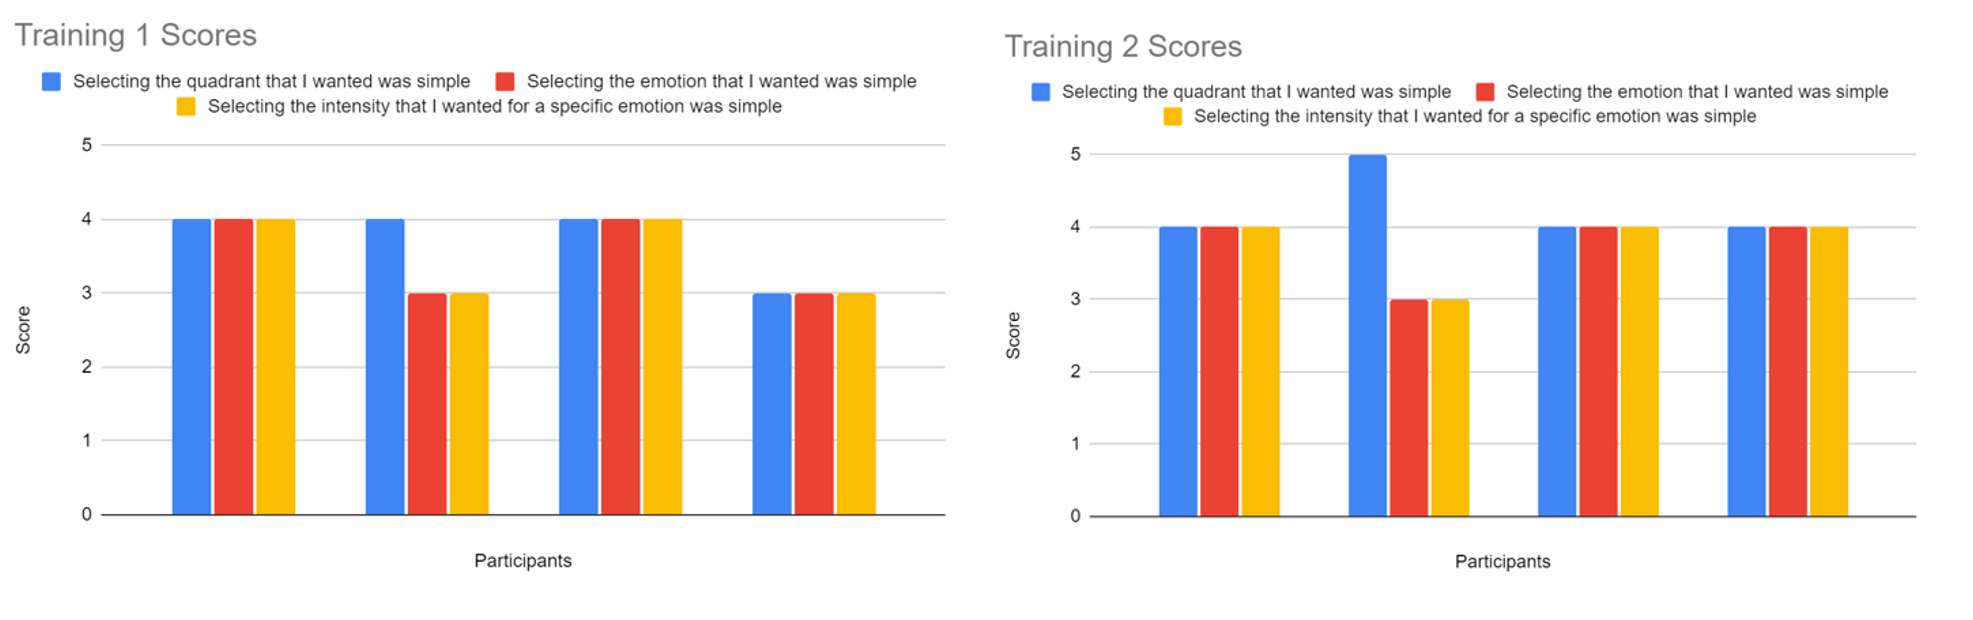
\includegraphics[width=16cm]{img/appendix/usability_condition_A.png}
\centering
\caption{Usability scores for training in condition A (joystick)}\label{fig:usbility_condition_A}
\end{figure}

\begin{figure}[!htb]
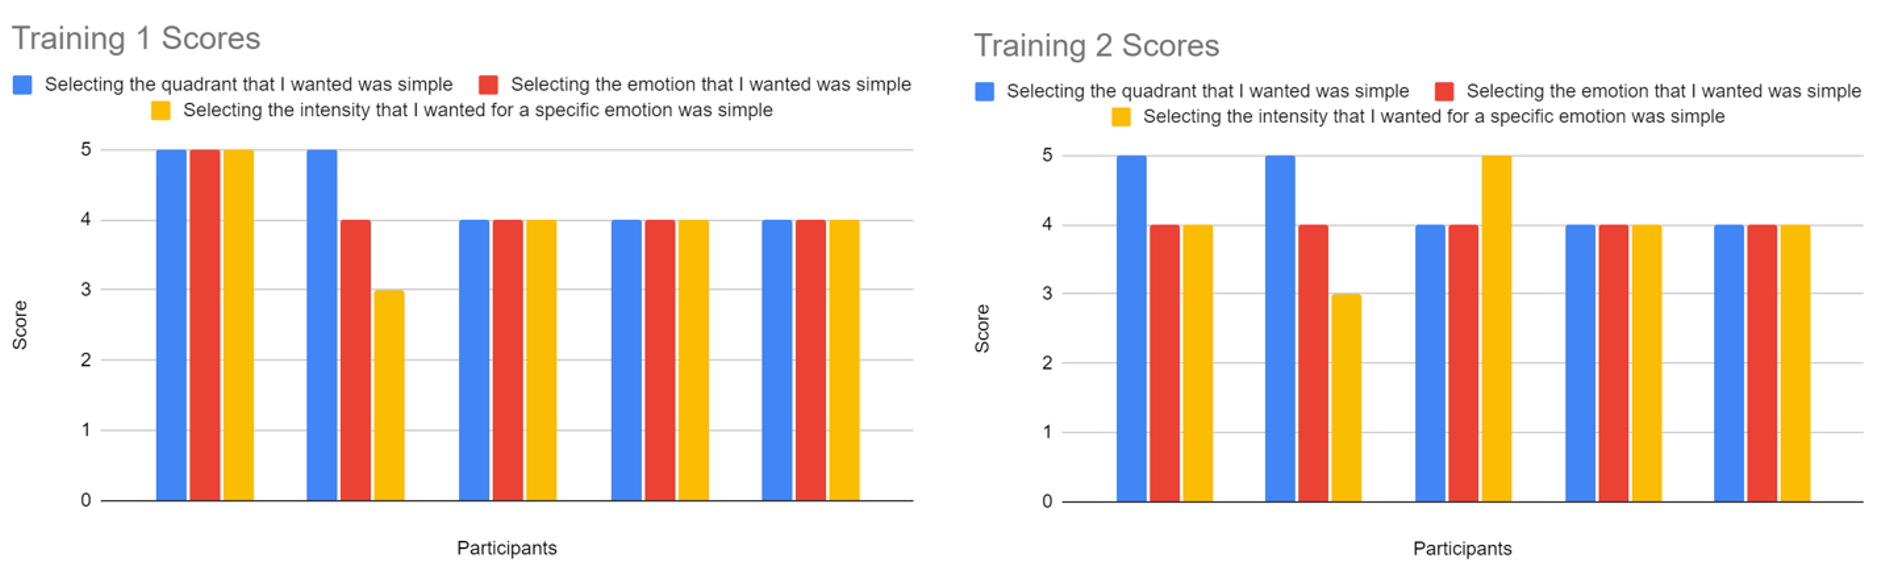
\includegraphics[width=16cm]{img/appendix/usability_condition_B.png}
\centering
\caption{Usability scores for training in condition A (joystick)}\label{fig:usbility_condition_B}
\end{figure}

\begin{table}[!htb]
  \caption{Average usability scores for the two groups.}
  \label{tbl:table_usability__scores}
  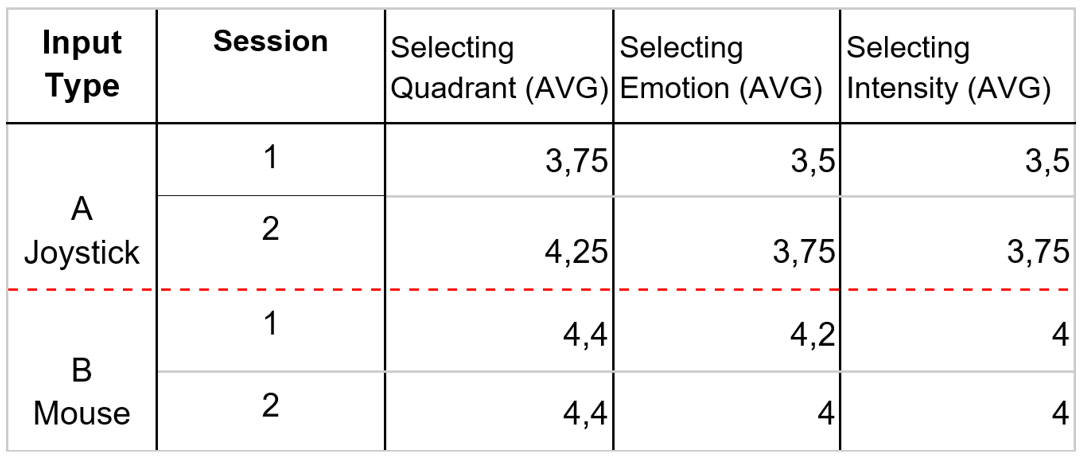
\includegraphics[width=\linewidth]{img/appendix/table_usability_scores.png}
\end{table}

\section{Methods}
\label{sec:appendix_A2}

\subsection{Participants infographic}
\label{sec:appendix_A2.1}

\begin{figure}[!htb]
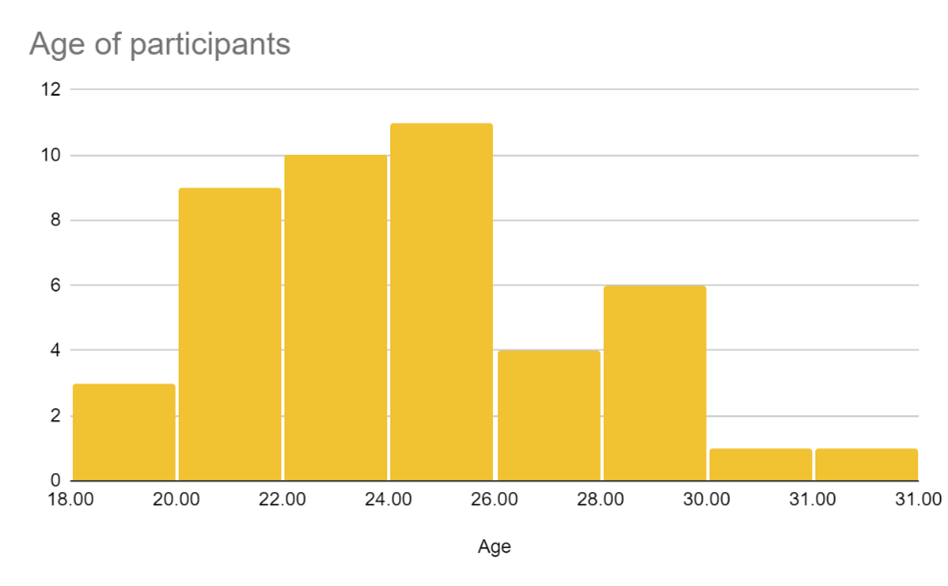
\includegraphics[width=14cm]{img/appendix/age_distribution.png}
\centering
\caption{Usability scores for training in condition A (joystick)}\label{fig:usbility_condition_B}
\end{figure}

\begin{figure}[!htb]
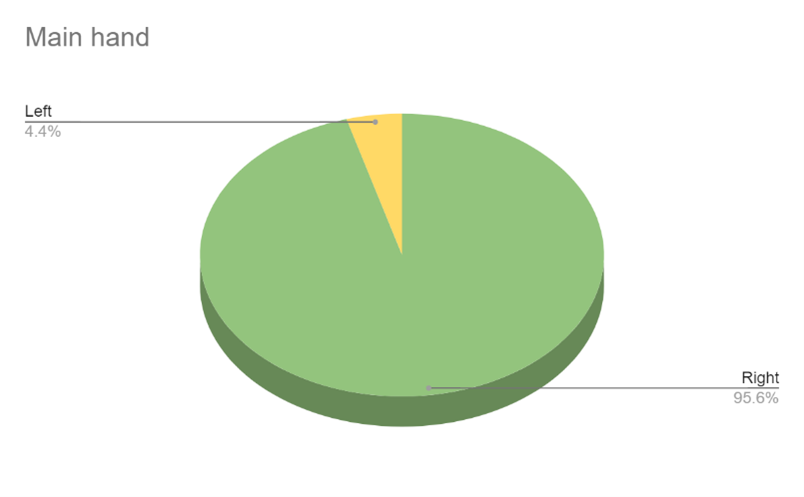
\includegraphics[width=14cm]{img/appendix/right_hand.png}
\centering
\caption{Usability scores for training in condition A (joystick)}\label{fig:usbility_condition_B}
\end{figure}

\subsection{Emotion-Music playlist}
\label{sec:appendix_A2.2}

High Arousal / High Valence (HAHV)
\begin{itemize}
\item  (High arousal, medium positive valence) Excitement- Weapon of choice by Fatboy Slim
\item  (Medium positive arousal, high valence) Happiness - Love Today by Mika
\end{itemize}

High Arousal / High Valence (LAHV)
\begin{itemize}
\item  (Medium negative Arousal, high valence) Satisfaction - Nasty Naughty Boy, by Christina Aguilera
\item 	 (Low arousal, medium positive valence) Relaxation – Amber by 311
\end{itemize}

High Arousal / High Valence (LALV)
\begin{itemize}
\item  (Medium negative arousal, High negative valence) Depression - Last Flowers by Radiohead
\item  (Low arousal, Medium negative valence) Sadness – Hurt by Johnny Cash
\end{itemize}

High Arousal / High Valence (HALV)
\begin{itemize}
\item  (Medium positive arousal, High negative valence) Anger – Threshold by Slayer
\item  (High positive arousal, Medium negative valence) Anxiety - Trapped Under Ice by Believe
\end{itemize}

Other songs were used in the training sessions, but no labelling is provided as their only purpose was 
to teach the users how to use the EA app GUI.
\begin{itemize}
\item  The white stripes - Seven Nation Army
\item  Gary Jules - Mad World
\item  Oren Lavie - Her morning elegance
\item  The Cranberries - Zombie
\item  Maneskin - I wanna be your slave
\item  Rage against the machine - Killing in the name of
\end{itemize}



\section{Intermediate experiments}
\label{sec:appendix_A3}
During the development of the classification pipeline, several intermediate experiments were run to
explore the data, the methodologies, and the different classifiers. The dataset of each subject was 
explored singularly, but only some examples are reported below

\subsection{Subject-dependent experiment with Sequential Features Selection}
\label{sec:appendix_A3.1}
\begin{table}[h!]
  \caption{Manually tuned hyper-paramters for MLP.}
  \label{tbl:mlp_initial_parameters}
  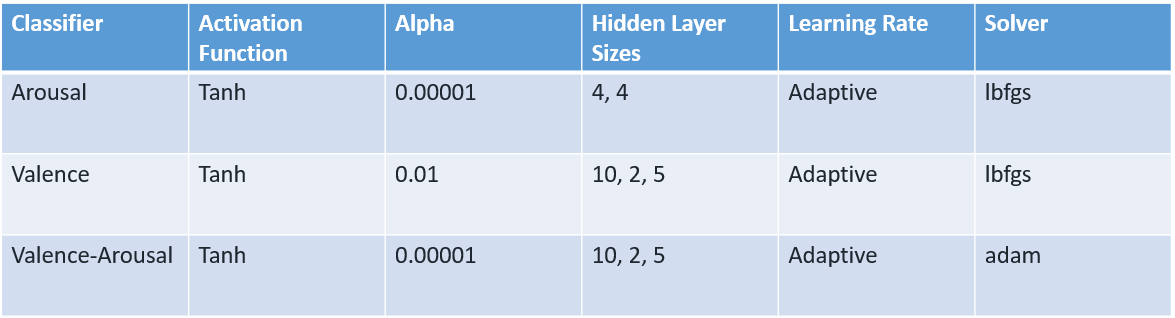
\includegraphics[width=\linewidth]{img/appendix/mlp_initial_parameters.png}
\end{table}

\begin{table}[h!]
  \caption{Manually tuned hyper-paramters for SVM.}
  \label{tbl:svm_initial_parameters}
  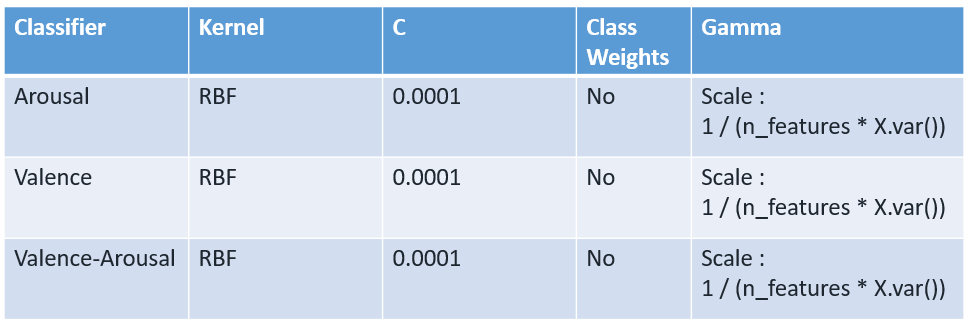
\includegraphics[width=\linewidth]{img/appendix/svm_initial_parameters.png}
\end{table}

\begin{table}[h!]
  \caption{Average cross-validated accuracy for each classifier and listening condition using SFS.}
  \label{tbl:sfs_cv_experiment}
  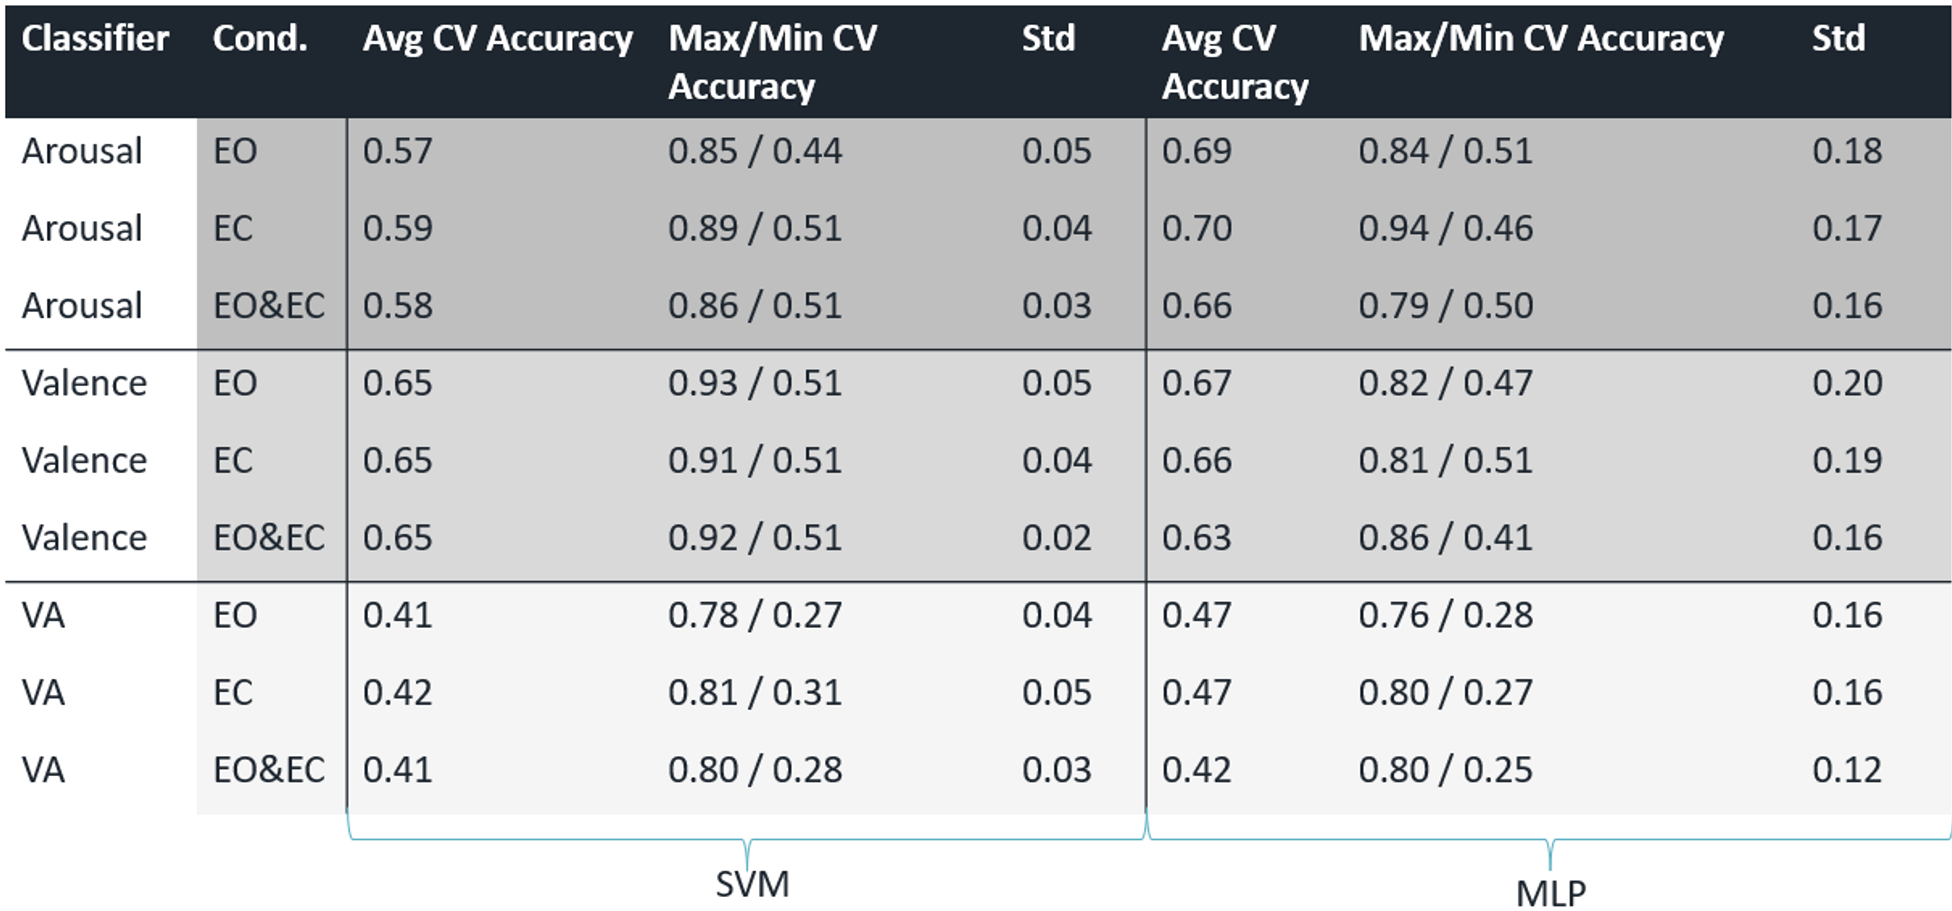
\includegraphics[width=\linewidth]{img/appendix/sfs_cv_experiment.png}
\end{table}

\begin{table}[h!]
  \caption{Most frequently selected features using SFS, renamed TOP5 features.}
  \label{tbl:sfs_features}
  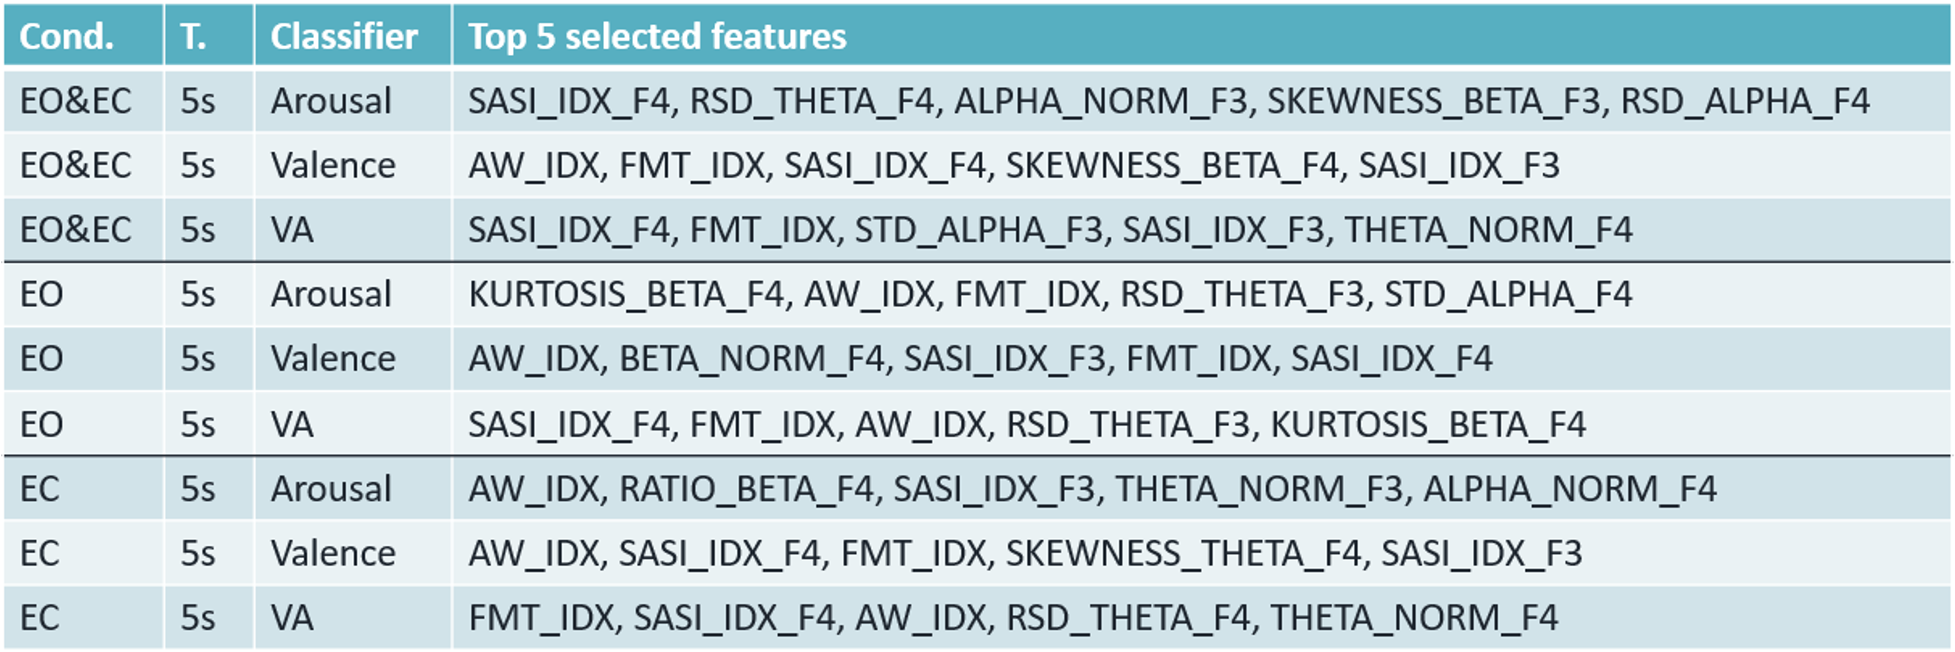
\includegraphics[width=\linewidth]{img/appendix/sfs_features.png}
\end{table}


\subsection{Subject-dependent experiment with TOP5 features}
\label{sec:appendix_A3.2}

\begin{table}[h!]
  \caption{Average cross-validated accuracy for each classifier and listening condition using TOP5 features.}
  \label{tbl:top5_cv_experiment}
  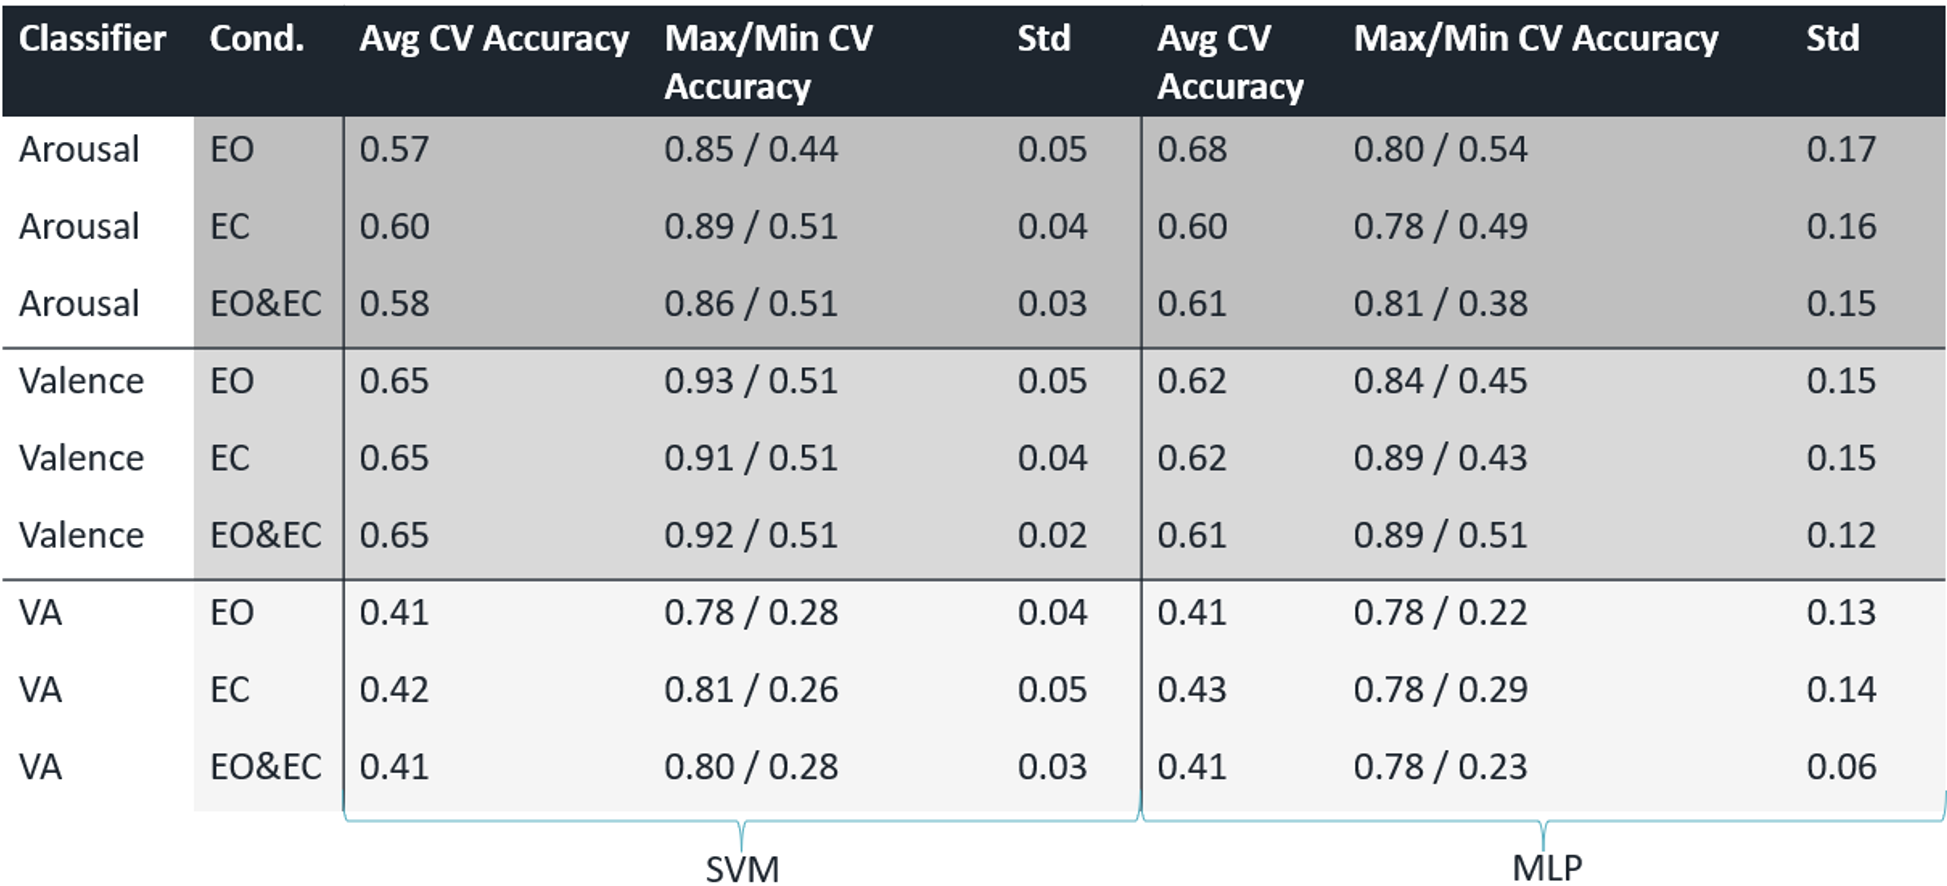
\includegraphics[width=\linewidth]{img/appendix/top5_cv_experiment.png}
\end{table}


\subsection{Example of unbalanced dataset for arousal classification}
\label{sec:appendix_A3.3.1}

\begin{figure}[!htb]
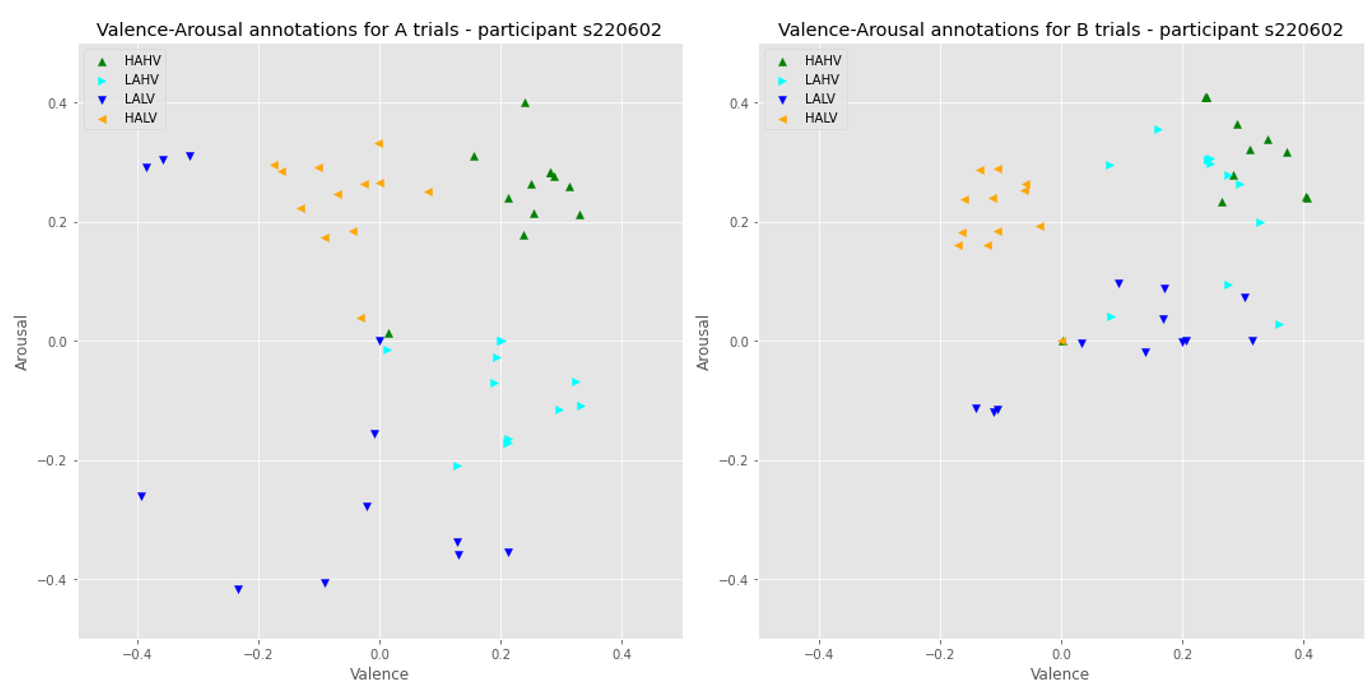
\includegraphics[width=16cm]{img/appendix/arousal_unbalanced.png}
\centering
\caption{Summary of annotation session for participant s220602. The labels are color coded according to the pre-labelled 
VA class of each song.}\label{fig:arousal_unbalanced}
\end{figure}

\begin{figure}[!htb]
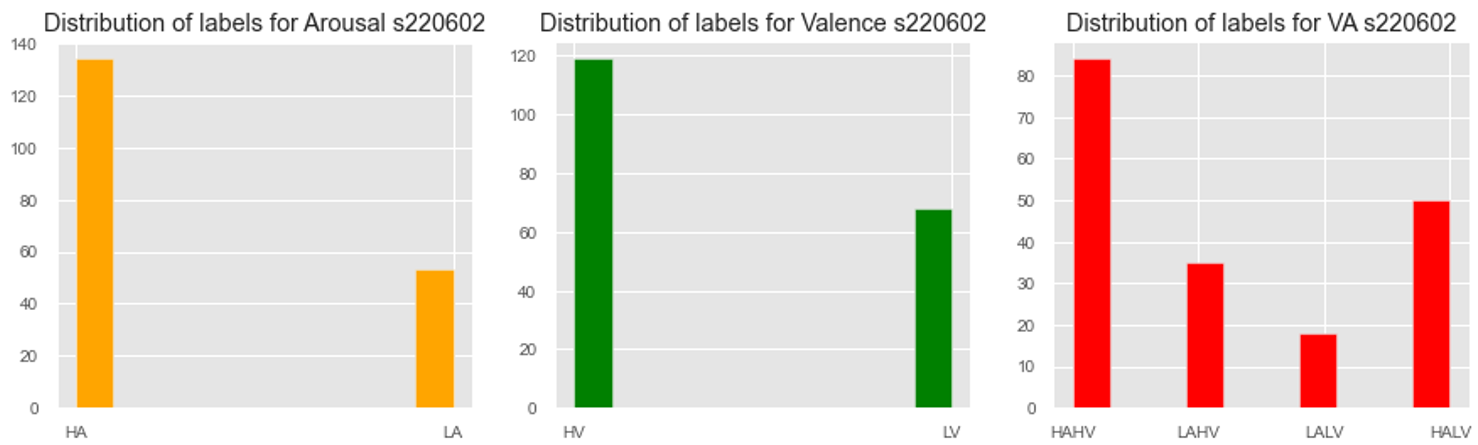
\includegraphics[width=16cm]{img/appendix/arousal_unbalanced_distribution.png}
\centering
\caption{Labels distribution of participant s220602. The LA* classes summed up are ~1/4 of the entire dataset.}\label{fig:arousal_unbalanced_distribution}
\end{figure}

\begin{figure}[!htb]
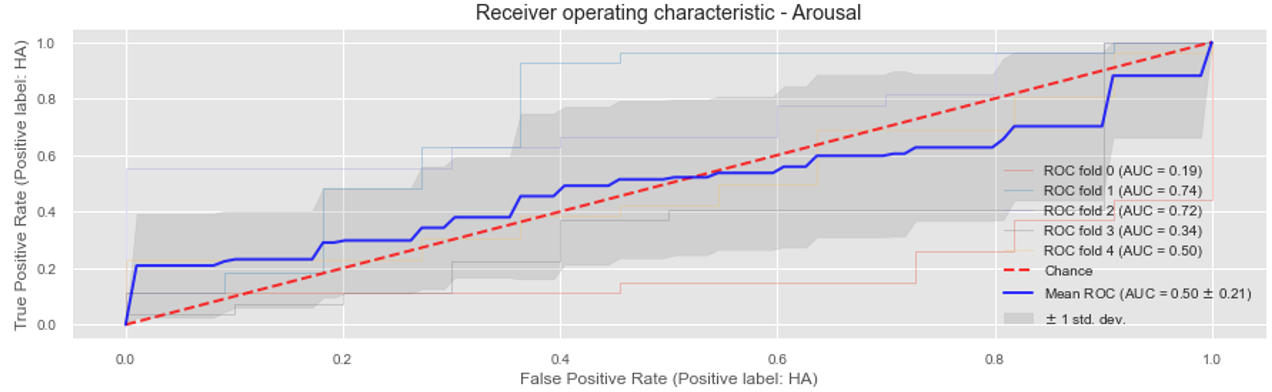
\includegraphics[width=16cm]{img/appendix/arousal_unbalanced_roc_svm.png}
\centering
\caption{Cross-validated ROC curve for participant s220602 for arousal classification using SVM.}\label{fig:arousal_unbalanced_roc_svm}
\end{figure}

\begin{figure}[!htb]
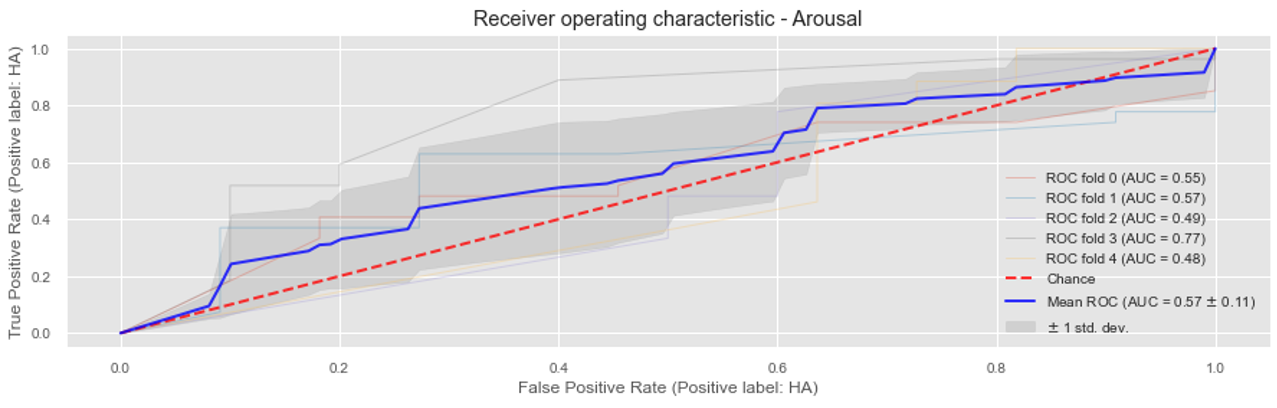
\includegraphics[width=16cm]{img/appendix/arousal_unbalanced_roc_mlp.png}
\centering
\caption{Cross-validated ROC curve for participant s220602 for arousal classification using MLP.}\label{fig:arousal_unbalanced_roc_mlp}
\end{figure}

\begin{figure}[!htb]
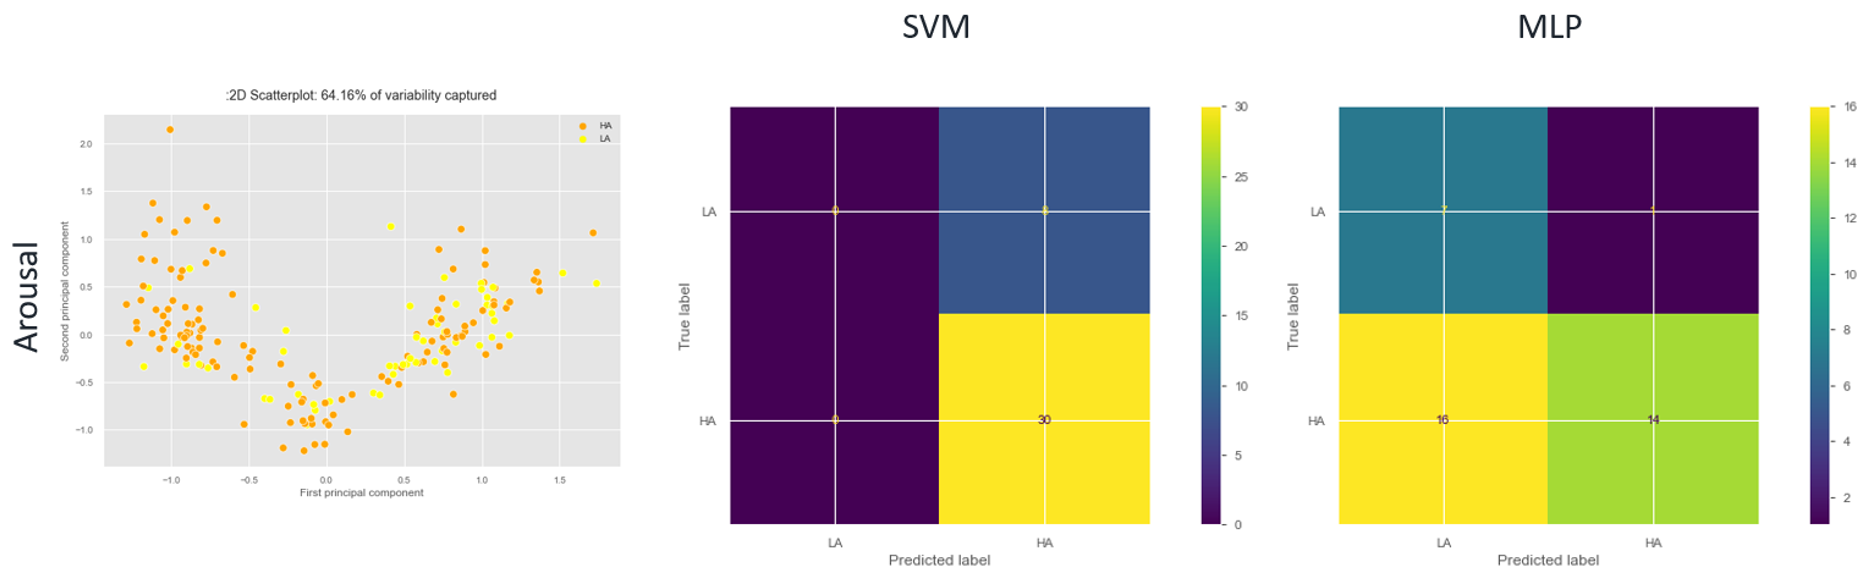
\includegraphics[width=16cm]{img/appendix/arousal_unbalanced_pca_confusion.png}
\centering
\caption{PCA (left) and confusion matrices (right) of s220602 participant with unbalanced labels for emotional arousal 
classification.}\label{fig:arousal_unbalanced_pca_confusion}
\end{figure}

\subsection{Example of unbalanced dataset for valence classification}
\label{sec:appendix_A3.3.2}

\begin{figure}[!htb]
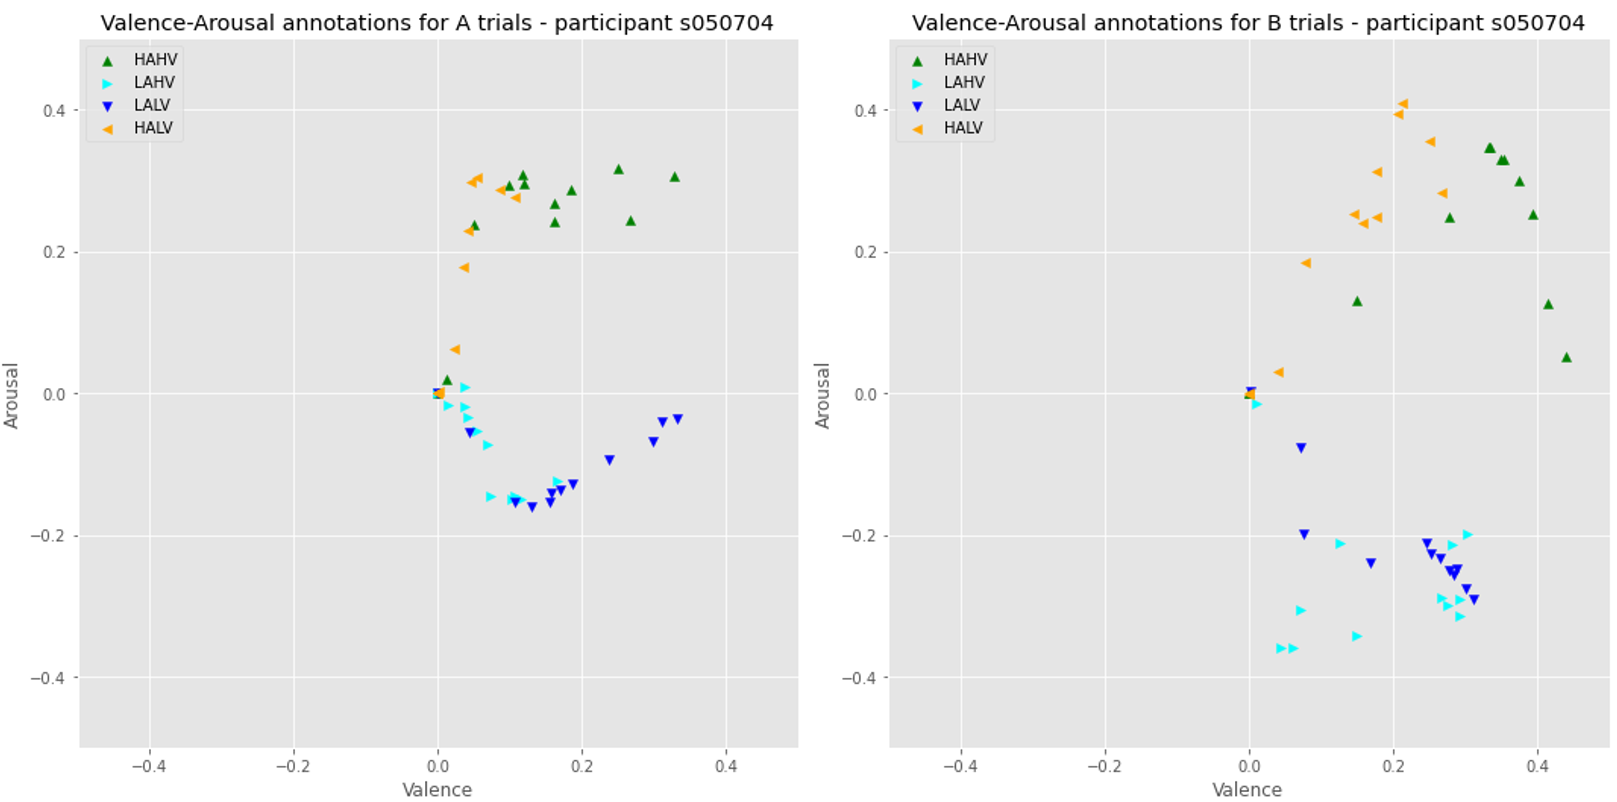
\includegraphics[width=16cm]{img/appendix/valence_unbalanced.png}
\centering
\caption{Summary of annotation session for participant s050704. The labels are color coded according to the pre-labelled 
VA class of each song.}\label{fig:valence_unbalanced}
\end{figure}

\begin{figure}[!htb]
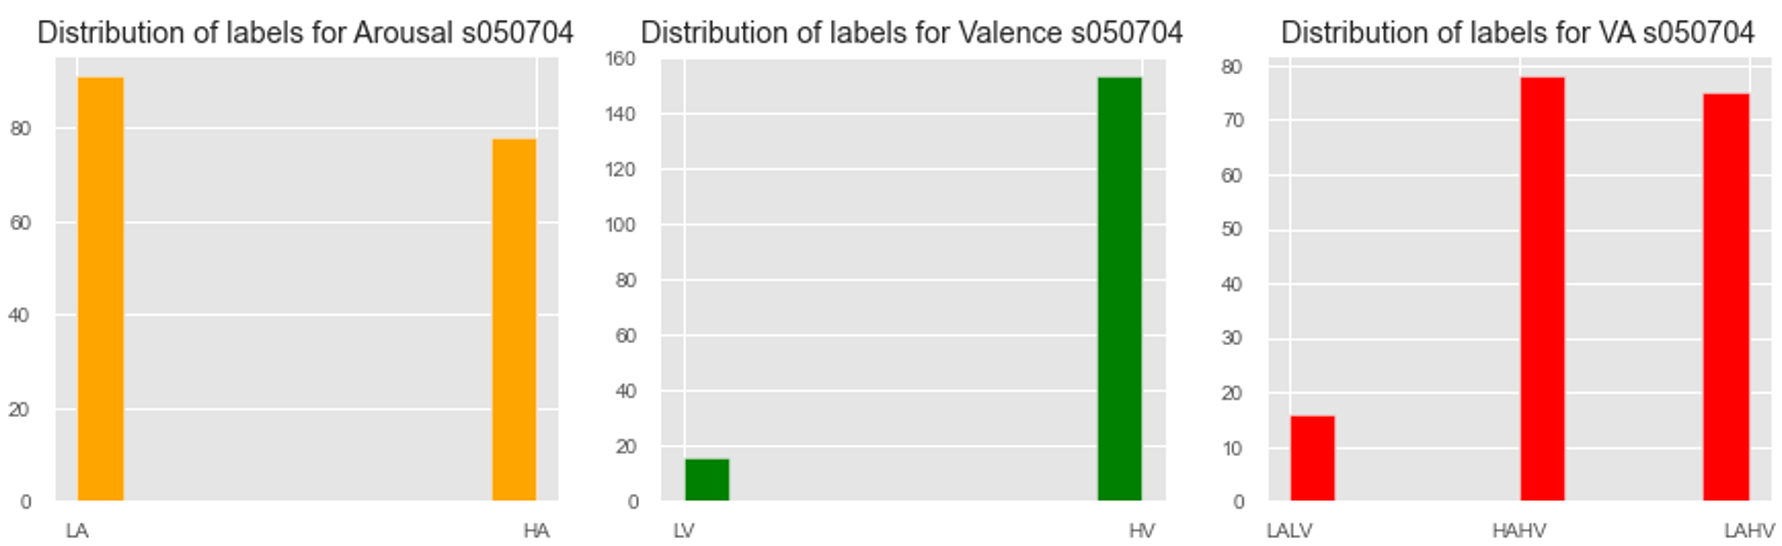
\includegraphics[width=16cm]{img/appendix/valence_unbalanced_distribution.png}
\centering
\caption{Labels distribution of participant s050704. The class HALV is completely missing.}\label{fig:valence_unbalanced_distribution}
\end{figure}

\begin{figure}[!htb]
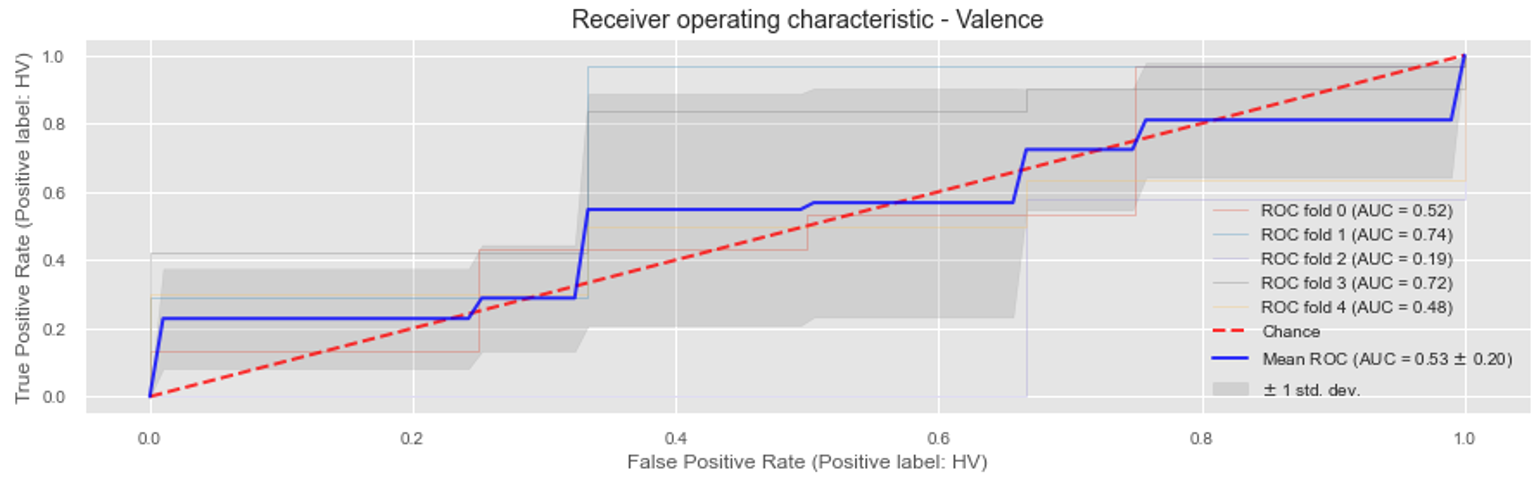
\includegraphics[width=16cm]{img/appendix/valence_unbalanced_roc_svm.png}
\centering
\caption{Cross-validated ROC curve for participant s050704 for valence classification using SVM.}\label{fig:valence_unbalanced_roc_svm}
\end{figure}

\begin{figure}[!htb]
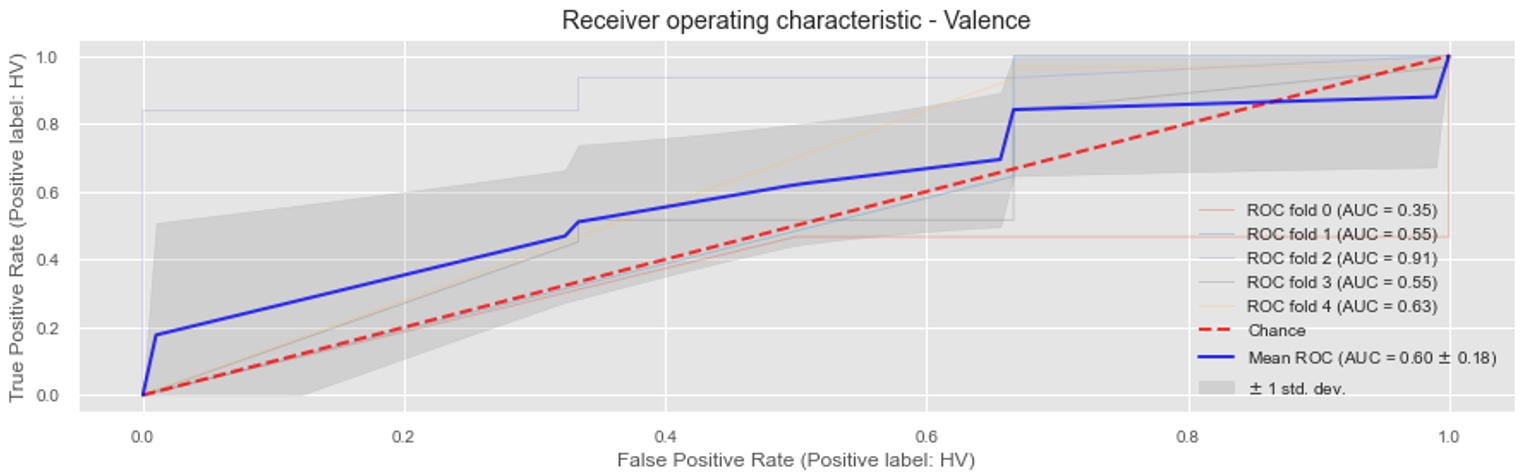
\includegraphics[width=16cm]{img/appendix/valence_unbalanced_roc_mlp.png}
\centering
\caption{Cross-validated ROC curve for participant s050704 for valence classification using MLP.}\label{fig:valence_unbalanced_roc_mlp}
\end{figure}

\begin{figure}[!htb]
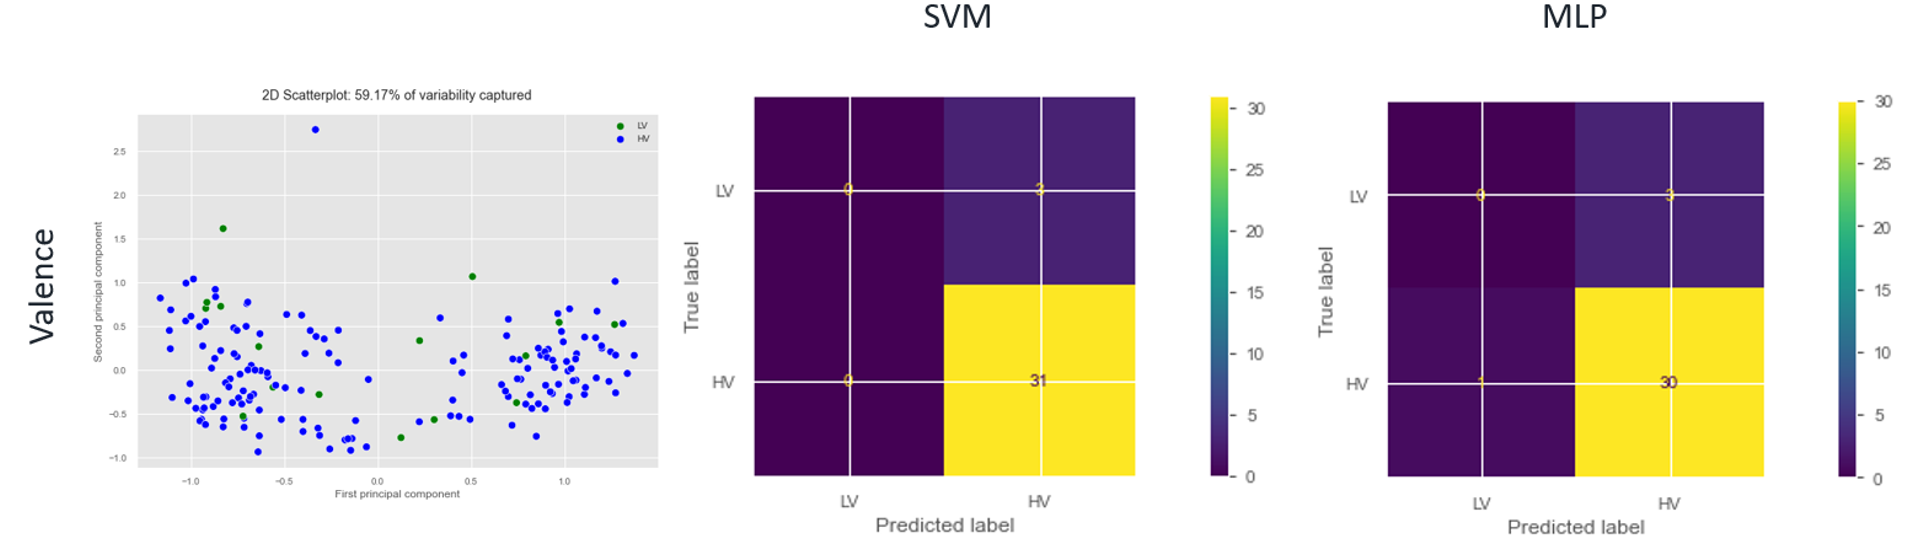
\includegraphics[width=16cm]{img/appendix/valence_unbalanced_pca_confusion.png}
\centering
\caption{PCA (left) and confusion matrices (right) of s050704 participant with unbalanced labels for emotional valence 
classification.}\label{fig:valence_unbalanced_pca_confusion}
\end{figure}

\subsection{Subject-independent experiment with Top5 features}
\label{sec:appendix_A3.4}
\begin{table}[h!]
  \caption{ Average cross-validated accuracy for each classifier and listening condition using TOP5 features.}
  \label{tbl:top5_cv_si_experiment}
  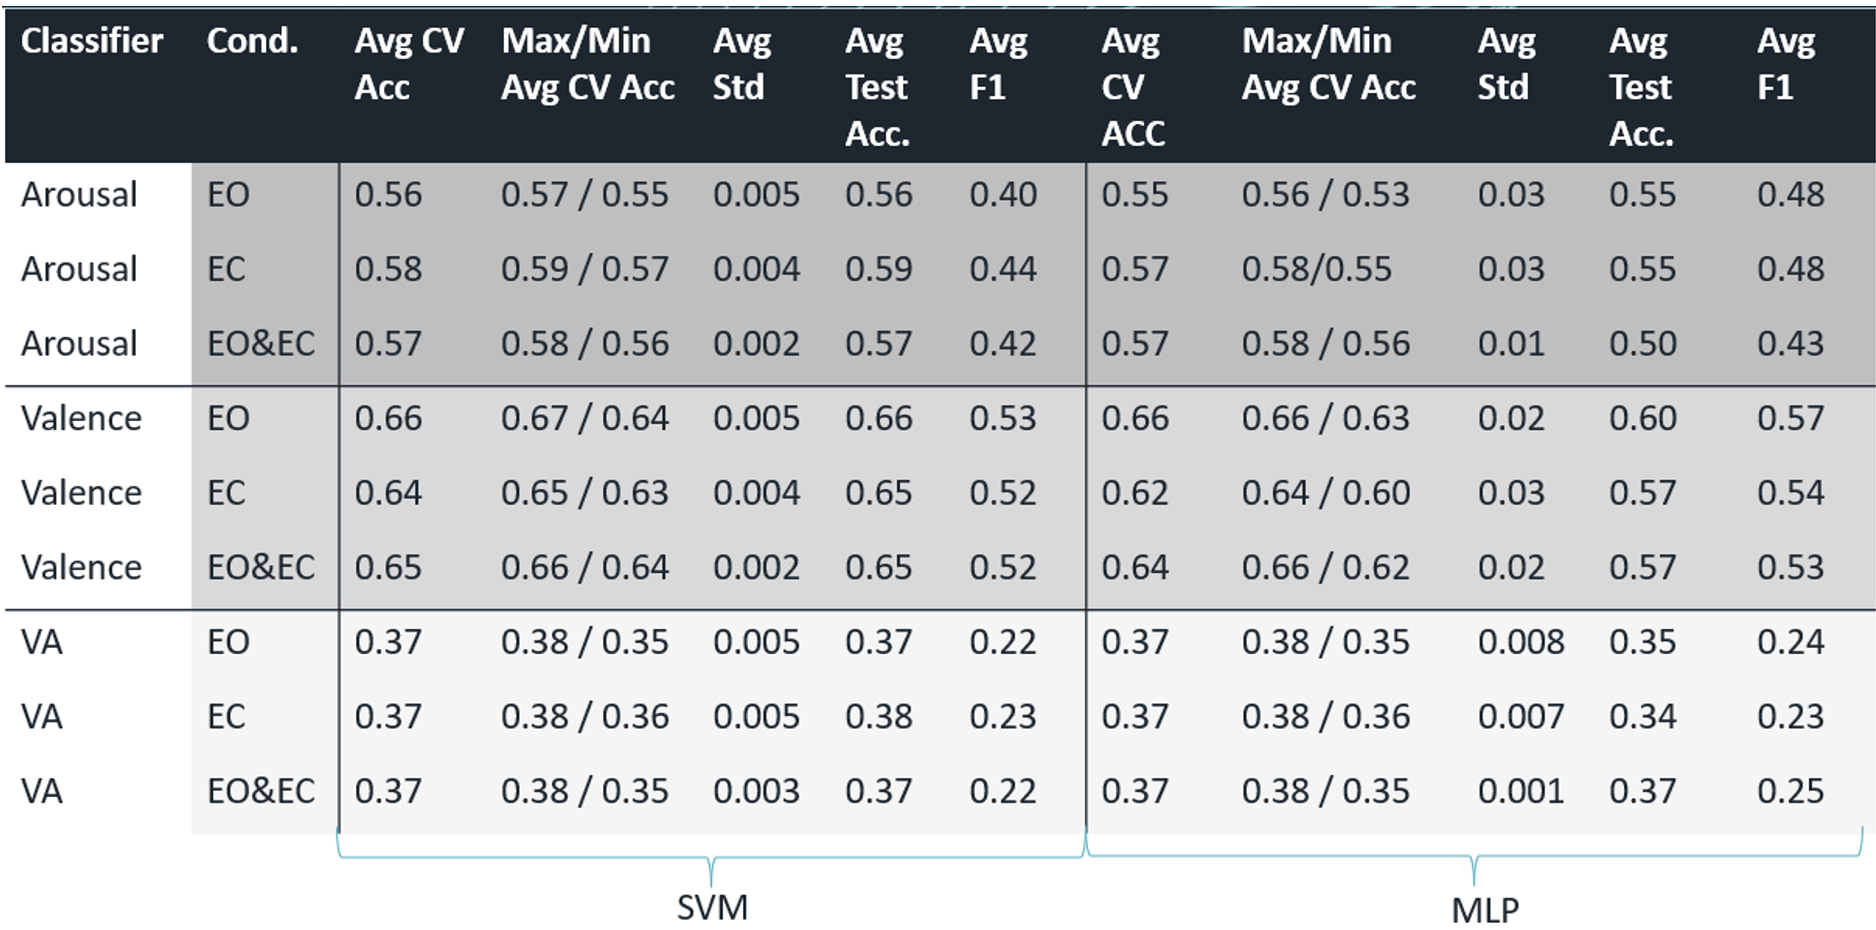
\includegraphics[width=\linewidth]{img/appendix/top5_cv_si_experiment.png}
\end{table}

\subsection{Subject-dependent experiment with "Max Accuracy" scoring strategy}
\label{sec:appendix_A3.5}

\begin{table}[h!]
  \caption{Arousal classification results using "accuracy" as scoring parameter for GridSearch. Learning models are highlighted in blue, over-fitted and under-fitted models are highlighted in yellow and orange, respectively.}
  \label{tbl:max_acc_arousal_results}
  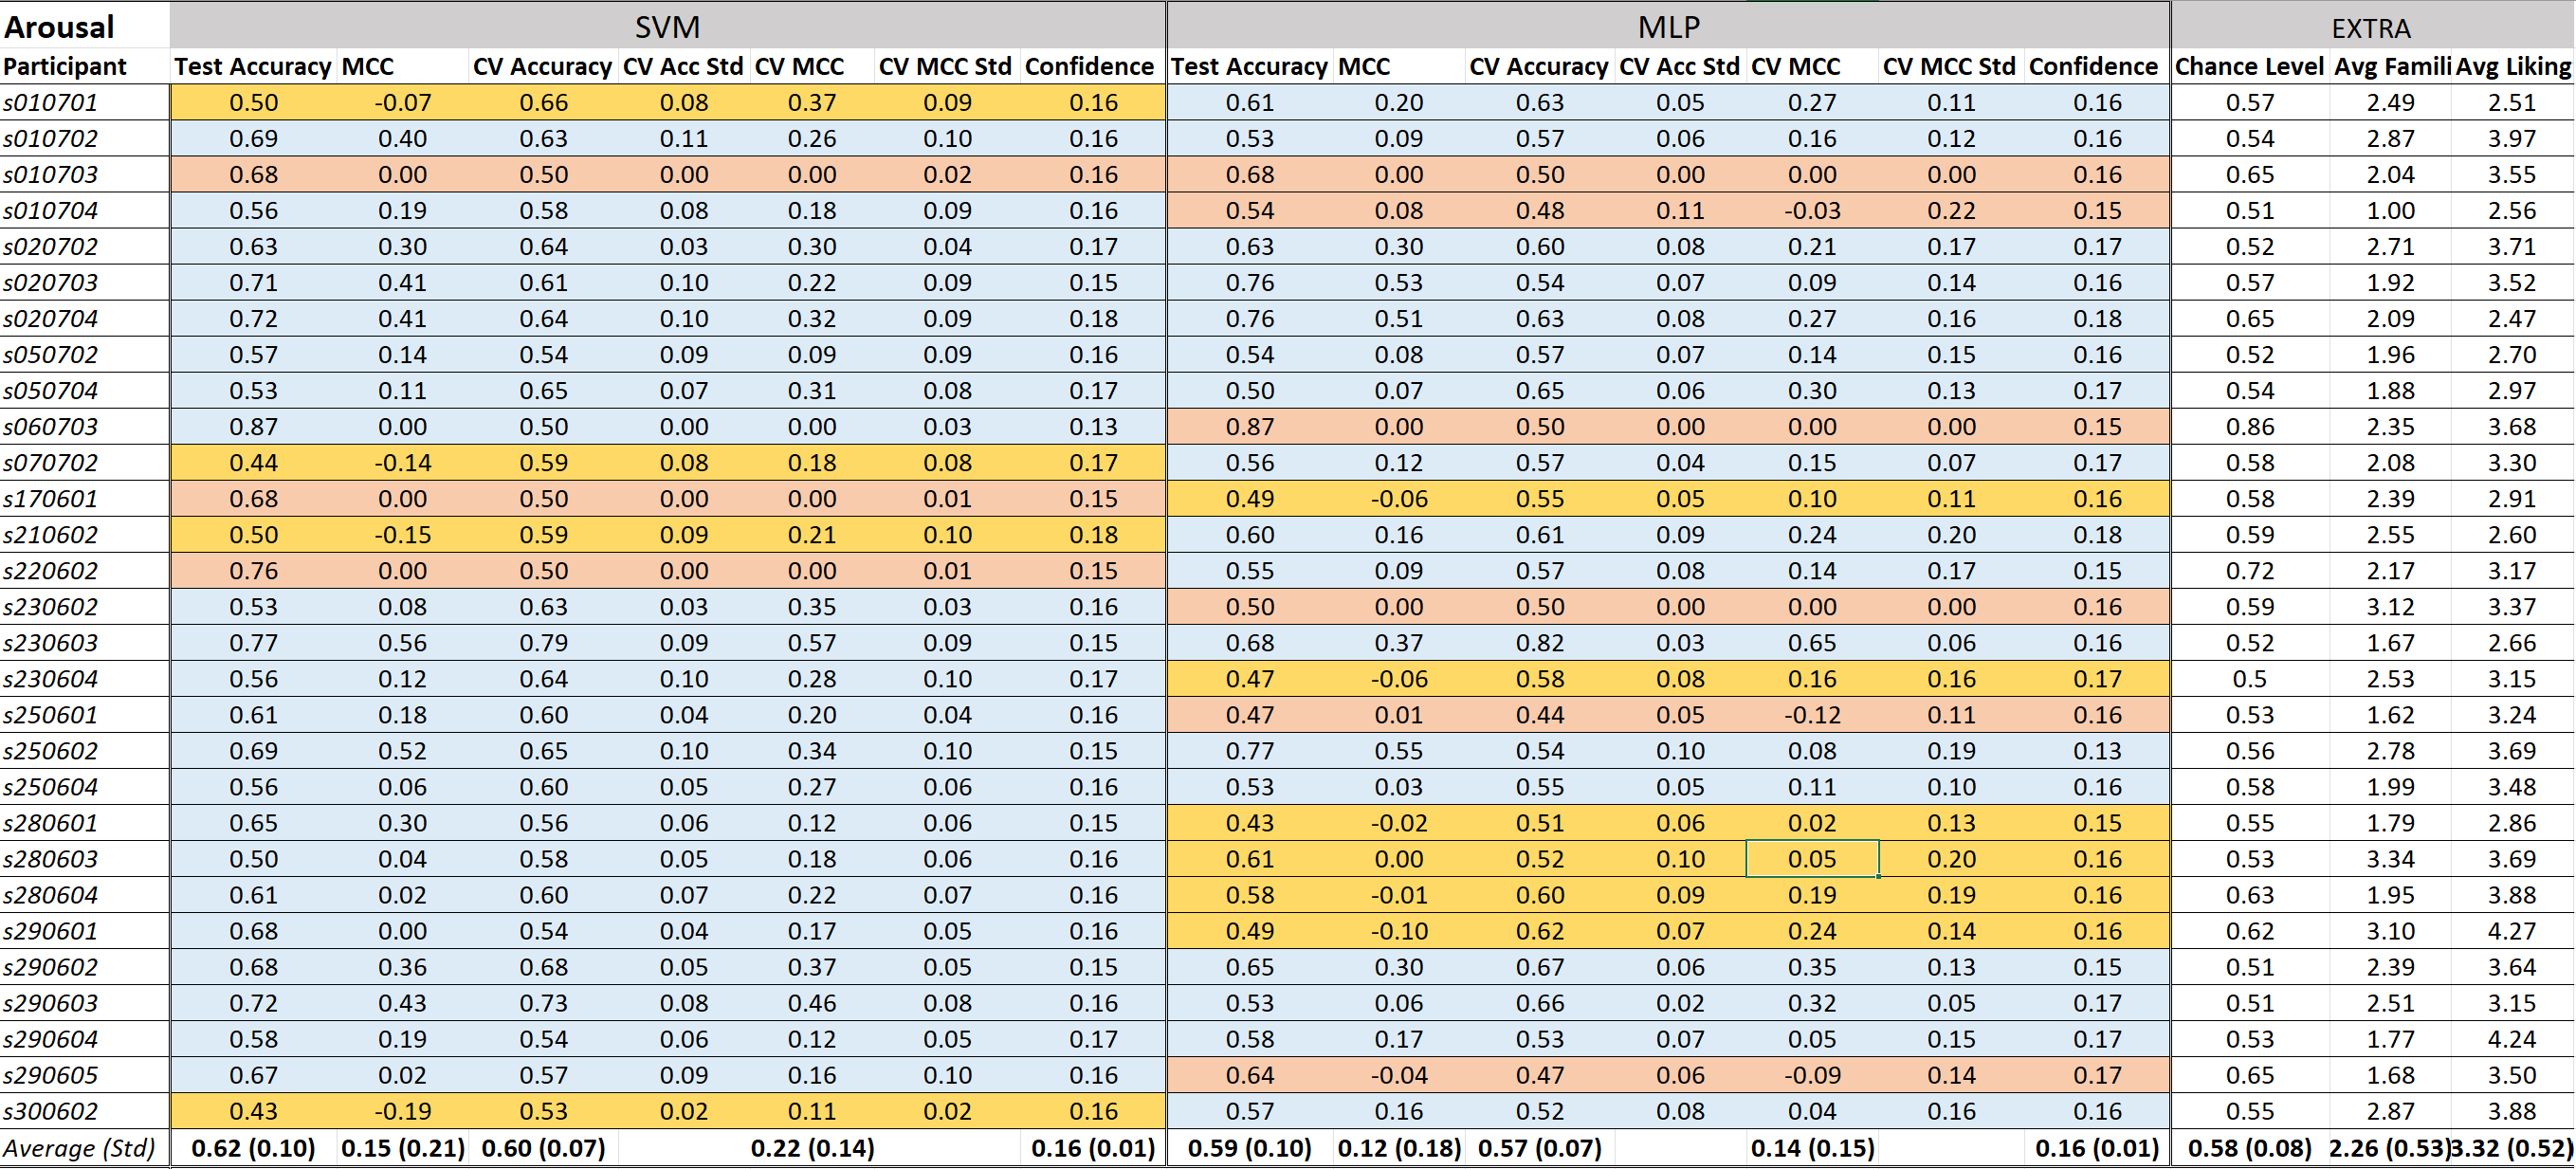
\includegraphics[width=\linewidth]{img/appendix/arousal_max_acc_results.png}
\end{table}

\begin{table}[h!]
  \caption{Valence classification results using "accuracy" as scoring parameter for GridSearch. Learning models are highlighted in blue, over-fitted and under-fitted models are highlighted in yellow and orange, respectively.}
  \label{tbl:max_acc_valence_results}
  \includegraphics[width=\linewidth]{img/appendix/valence_max_acc_results.png}
\end{table}


\section{Final experiment}
\label{sec:appendix_A4}

\begin{figure}[!htb]
\includegraphics[width=16cm]{img/appendix/final_experiment/experiment_test_recap.png}
\centering
\caption{Average Test Accuracy and MCC compare against majority class guessing.}\label{fig:experiment_test_recap}
\end{figure}

\begin{figure}[!htb]
\includegraphics[width=16cm]{img/appendix/final_experiment/experiment_cv_recap.png}
\centering
\caption{Average CV Accuracy and CV MCC compare against majority class guessing.}\label{fig:experiment_cv_recap}
\end{figure}

\subsection{Ranking of SVM classification performances for arousal classification}
\label{sec:appendix_A4.1}

\begin{figure}[!htb]
\includegraphics[width=16cm]{img/appendix/final_experiment/test_acc_mcc_arousal_svm.png}
\centering
\caption{Ranking of subject-dependent SVM models performances for arousal classification by Test MCC, descending.}\label{fig:test_acc_mcc_arousal_svm}
\end{figure}

\begin{figure}[!htb]
\includegraphics[width=16cm]{img/appendix/final_experiment/test_cv_acc_mcc_arousal_svm.png}
\centering
\caption{Ranking of subject-dependent SVM models performances for arousal classification by CV MCC, descending.}\label{fig:test_cv_acc_mcc_arousal_svm}
\end{figure}

\subsection{Ranking of MLP classification performances for arousal classification}
\label{sec:appendix_A4.2}

\begin{figure}[!htb]
\includegraphics[width=16cm]{img/appendix/final_experiment/test_acc_mcc_arousal_mlp.png}
\centering
\caption{Ranking of subject-dependent MLP models performances for arousal classification by Test MCC, descending.}\label{fig:test_acc_mcc_arousal_mlp}
\end{figure}

\begin{figure}[!htb]
\includegraphics[width=16cm]{img/appendix/final_experiment/test_cv_acc_mcc_arousal_mlp.png}
\centering
\caption{Ranking of subject-dependent MLP models performances for arousal classification by CV MCC, descending.}\label{fig:test_cv_acc_mcc_arousal_mlp}
\end{figure}

\subsection{Ranking of SVM classification performances for valence classification}
\label{sec:appendix_A4.3}

\begin{figure}[!htb]
\includegraphics[width=16cm]{img/appendix/final_experiment/test_acc_mcc_valence_svm.png}
\centering
\caption{Ranking of subject-dependent SVM models performances for valence classification by Test MCC, descending.}\label{fig:test_acc_mcc_valence_svm}
\end{figure}

\begin{figure}[!htb]
\includegraphics[width=16cm]{img/appendix/final_experiment/test_cv_acc_mcc_valence_svm.png}
\centering
\caption{Ranking of subject-dependent SVM models performances for valence classification by CV MCC, descending.}\label{fig:test_cv_acc_mcc_valence_svm}
\end{figure}

\subsection{Ranking of MLP classification performances for valence classification}
\label{sec:appendix_A4.4}

\begin{figure}[!htb]
\includegraphics[width=16cm]{img/appendix/final_experiment/test_acc_mcc_valence_mlp.png}
\centering
\caption{Ranking of subject-dependent MLP models performances for valence classification by Test MCC, descending.}\label{fig:test_acc_mcc_valence_mlp}
\end{figure}

\begin{figure}[!htb]
\includegraphics[width=16cm]{img/appendix/final_experiment/test_cv_acc_mcc_valence_mlp.png}
\centering
\caption{Ranking of subject-dependent MLP models performances for valence classification by CV MCC, descending.}\label{fig:test_cv_acc_mcc_valence_mlp}
\end{figure}


\end{appendix}


\end{document}
